\chapter{An EFT interpretation of STXS measurements}
\label{chap:eft}

\section{Introduction}

Effective field theories were introduced in section \ref{sec:theory_eft} as a model-independent approach to constraining BSM physics. In EFT, new BSM states are assumed to exist with masses at an energy scale, $\Lambda$, far beyond the electroweak energy scale, $v$~=~246~GeV. The dynamics introduced by the BSM states can be parametrised at low energies ($E \sim v$) using higher-dimensional operators built up from the SM fields, where the operators are confined to respect both the symmetries and gauge invariance of the SM. This expansion of the SM Lagrangian, shown explicitly in equation \ref{eq:eft_expansion}, is fully general and thus can be used to constrain a wide class of BSM theories that reduce to the SM at low energies. The Wilson coefficients, $w_p$, directly parametrise the contribution from operator, $\mathcal{O}_p$, and by constraining these coefficients it is possible to infer both the strength and potential type of new BSM interactions. Ultimately, the final constraints on the Wilson coefficients can then be systematically matched to explicit UV-complete BSM theories~\cite{Marzocca:2020jze}.

This chapter details the application of EFT to Higgs boson property measurements at CMS. The Higgs Effective Lagrangian (HEL) is used as the language to encode modifications to Higgs boson properties from BSM physics~\cite{Contino:2013kra,Alloul:2013naa}. This interpretation is applied to the most recent CMS Higgs boson combination, documented in Ref.~\cite{CMS-PAS-HIG-19-005}, which combines the measurements of cross sections in the STXS framework from multiple decay channels. In doing so, a more complete set of EFT operators, affecting multiple Higgs boson interactions with other particles, can be constrained. Additionally, by performing the EFT interpretation \textit{in-house}, the fit uses the full likelihood surface, meaning no assumptions regarding the Gaussian nature of the likelihood are required.

In contrast to the $\kappa$-framework discussed in section \ref{sec:results_kappa}, the EFT approach is based on a fully consistent expansion of the SM Lagrangian. As a result, the EFT dependence can be extended from simple normalisation effects on inclusive production mode cross sections, to also capture shape variations in the kinematic distributions e.g. \ptH, \mjj, $N_{\rm{jets}}$ etc. In this interpretation, the parametrisation is defined at the granularity of the STXS framework. This ensures that the kinematic information available in STXS measurements is used to better constrain BSM physics. Additionally, the $\kappa$-framework defines coupling modifiers at LO. The EFT approach on the other hand is systematically improvable by computing higher-order contributions to the EFT predictions~\cite{Degrande:2020evl}. The interpretation shown in this chapter only considers EFT effects at LO, however the future transition to higher-orders is briefly discussed in section \ref{sec:eft_improving}.

The structure of this chapter is as follows: firstly the HEL model is described in section \ref{sec:eft_hel} and the choice of operators considered in the fit is motivated. Following this, the CMS Higgs combination~\cite{CMS-PAS-HIG-19-005} is detailed in section \ref{sec:eft_combination}, including the full set of input analyses and the extension to the statistical inference techniques introduced in chapter \ref{chap:hgg_stats}. Section \ref{sec:eft_parametrisation} discusses the EFT parametrisation of the signal yield, where the cross sections and branching fractions are expressed as functions of the Wilson coefficients, $\mu^{i,f}(\vec{w})$. These functions are then used to fit the Wilson coefficients to Higgs boson measurements, and extract their respective confidence intervals. This is performed using both a simplified re-interpretation procedure and using the full likelihood fit, described in sections \ref{sec:eft_simplified} and \ref{sec:eft_results}, respectively. Finally, the future of EFT measurements in CMS and how they can be improved is discussed in section \ref{sec:eft_improving}.

\section{Higgs Effective Lagrangian}\label{sec:eft_hel}

% \textbf{This is incorrect! Re-do! SILH is a SMEFT, intoduce it as such. Observed scalar in doublet.}

The Higgs Effective Lagrangian (HEL) model~\cite{Alloul:2013naa} is a SMEFT, which corresponds to a partial implementation of the complete SILH basis~\cite{Giudice:2007fh,Contino:2013kra}, encompassing all operators at dimension-6 related to the Higgs sector. The perturbative expansion is defined in terms of the CP-even complex scalar Higgs field, H, and therefore assumes the scalar sector follows the SU$_{\rm{L}}$(2) doublet nature in the SM. The model is constructed by extending the SM Lagrangian with 39 flavour independent dimension-6 operators, $\mathcal{O}^{(6)}_p$, as shown in equation \ref{eq:hel_expansion}, such that new BSM dynamics in the Higgs sector would manifest itself as deviations from zero in the HEL Wilson coefficients, $w_p$. Operators representing four-fermion interactions are not included.

% This choice reflects minimal assumptions in the scalar sector, and therefore can account for the possibility that the Higgs boson may deviate from the SU$_{\rm{L}}$(2) doublet nature in the SM, such as in composite Higgs models~\cite{} and theories with extra dimensions~\cite{}. The implication of this choice is that unitarity is not exactly preserved; this is not essential for EFT as long as unitarity is preserved up to the cut-off scale, $\Lambda$.

%The HEL model extends the SM Lagrangian by introducing 39 flavour independent dimension-6 operators, $\mathcal{O}^{(6)}_p$, as shown in equation \ref{eq:hel_expansion}, such that new BSM dynamics in the Higgs sector would manifest itself as deviations from zero in the Wilson coefficients, $w_p$. Operators representing four-fermion interactions are not included. 

\begin{equation}\label{eq:hel_expansion}
    \mathcal{L}_{\rm{HEL}} = \mathcal{L}_{\rm{SM}} + \sum_p \frac{w_p}{\Lambda^2}\mathcal{O}^{(6)}_p .
\end{equation}

\noindent
Currently, there is insufficient data to constrain all directions of parameter space, $\vec{w}$. As a result, a subset of operators, $\{\mathcal{O}\}$  most relevant to the input Higgs boson measurements is considered. This choice ultimately introduces a model dependence into the interpretation, assuming the contribution from other operators is zero: 

\begin{equation}
  w_p=0 \; \forall \; \mathcal{O}_p \notin \{\mathcal{O}\}.   
\end{equation}

\noindent
The subset of operators considered in this interpretation is motivated below.

\subsection{Operator selection}\label{sec:eft_operator}
Non-zero contributions are considered in a total of eight dimension-6 operators,
\begin{equation}
    \{\mathcal{O}\} = \{\mathcal{O}_G,\mathcal{O}_A,\mathcal{O}_u,\mathcal{O}_d,\mathcal{O}_\ell,\mathcal{O}_{HW},\mathcal{O}_{WW},\mathcal{O}_B\},
\end{equation}
\noindent
where the explicit form of these operators in terms of the SM fields and the relevant Higgs boson interaction vertices are listed in Table~\ref{tab:hel_operators}. In this analysis, the nominal Wilson coefficients, $\vec{w}$, are redefined as dimensionless \textit{HEL parameters}, $\vec{c}$, which absorb the factor of $\Lambda^{-2}$. The definitions of the HEL parameters for each operator are also provided in Table~\ref{tab:hel_operators}. The operators $\mathcal{O}_G$ and $\mathcal{O}_A$ correspond to the effective Hgg and H$\gamma\gamma$ vertices, respectively. Since the interpretation presented here is a LO implementation of the HEL, the the ggH and \Hgg loops are not resolved into their SM structures and therefore only depend on $\mathcal{O}_G$ and $\mathcal{O}_A$.

This set of operators is chosen since the HEL parameters account for the leading CP-even terms in the scaling functions for the measured cross sections and branching fractions, and are not tightly constrained by existing measurements. CP-odd parameters are neglected as they do not enter the parametrisation at leading order in $1/\Lambda^2$, and since there is no splitting in the STXS framework that is sensitive to the Higgs boson CP (e.g. a splitting in $\Delta\phi_{jj}$) the dependence is completely degenerate with the corresponding CP-even terms at $1/\Lambda^4$.

The parameters, $c_{WW}$ and $c_B$ are fit together in the combination, $c_{WW}-c_B$, since the orthogonal combination ($S=c_{WW}+c_B$) is strongly constrained at zero by electroweak precision data~\cite{Ellis:2014jta}. Finally, the operator, $\mathcal{O}_{HB}$, is neglected. Despite having a sizeable impact on the measured quantities, the effects of $\mathcal{O}_{HB}$ are synonymous with $\mathcal{O}_{HW}$, without including additional differential measurements of the VH production mode cross or measurements of the \HZg decay channel. In conclusion, seven parameters of interest are defined:

\begin{equation}
    c_G, c_A, c_u, c_d, c_\ell, c_{HW}, c_{WW}-c_B.
\end{equation}

\begin{table}[htb!]
  \centering
  \scriptsize
  \renewcommand{\arraystretch}{2.5}
  \setlength{\tabcolsep}{3pt}
  \caption[Operator subset in the HEL interpretation]
  {
    The dimension-6 operator subset, $\{\mathcal{O}\}$, considered in the HEL interpretation. The definition of each operator is provided in terms of the SM field tensors. In addition, the corresponding HEL parameter is defined in terms of the nominal EFT Wilson coefficients. The final two columns show the affected Higgs boson interaction vertices and an example Feynman diagram of the EFT interaction. 
  }
  \label{tab:hel_operators}
%   \hspace*{-.5cm}
  \begin{tabular}{lcm{3cm}<{\centering}cm{4.5cm}<{\centering}}
    Operator & Definition & HEL Parameter & Relevant vertices & Example diagrams \\ \hline

    $\mathcal{O}_G$ & $|H|^2G^A_{\mu\nu}G^{A,\mu\nu}$ & $c_G=\frac{m_W^2}{g_s^2}\frac{w_G}{\Lambda^2}$ & Hgg & \vspace{.1cm}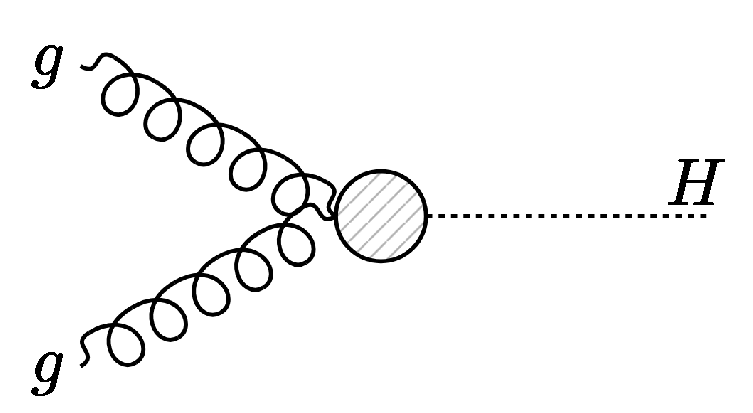
\includegraphics[width=2.5cm]{Figures/eft/eft_feynman/cG.pdf} \\

    $\mathcal{O}_A$ & $|H|^2B_{\mu\nu}B^{\mu\nu}$ & $c_A=\frac{m_W^2}{g^{'2}}\frac{w_A}{\Lambda^2}$ & H$\gamma\gamma$, HZZ & \vspace{.1cm}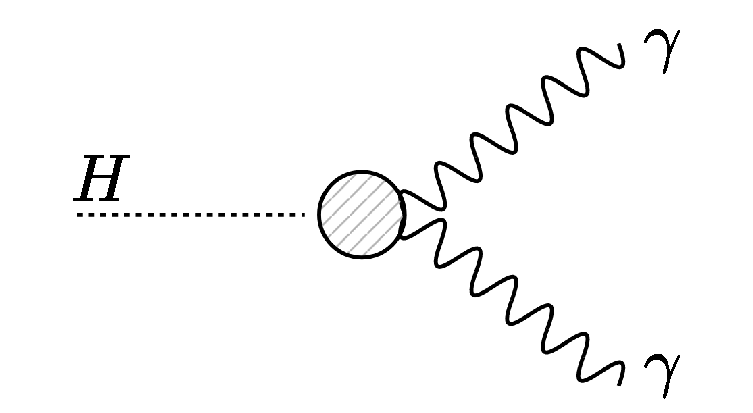
\includegraphics[width=2cm]{Figures/eft/eft_feynman/cA.pdf} \vspace{.1cm}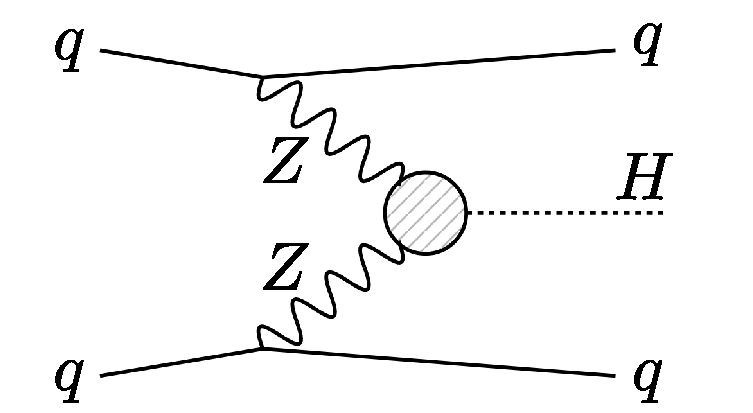
\includegraphics[width=2cm]{Figures/eft/eft_feynman/cB.pdf} \\

    $\mathcal{O}_u$ & $y_u|H|^2\bar{Q}_LH^{\dagger}u_R + {\rm{h.c.}}$ & $c_u=-v^2\frac{w_u}{\Lambda^2}$ & Htt & \vspace{.1cm}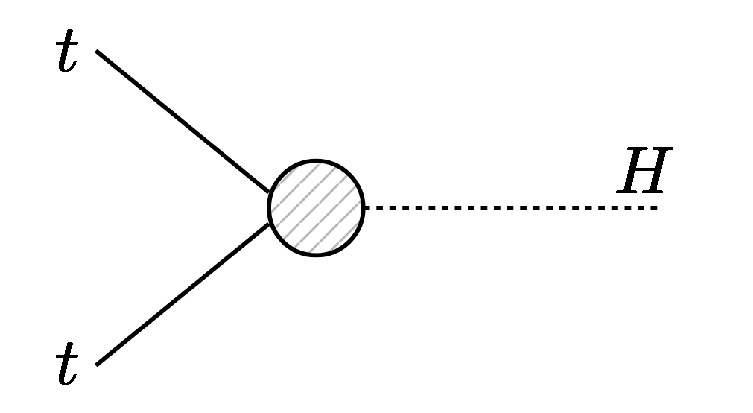
\includegraphics[width=2.5cm]{Figures/eft/eft_feynman/cu.pdf} \\

    $\mathcal{O}_d$ & $y_d|H|^2\bar{Q}_LH^{\dagger}d_R + {\rm{h.c.}}$ & $c_d=-v^2\frac{w_d}{\Lambda^2}$ & Hbb & \vspace{.1cm}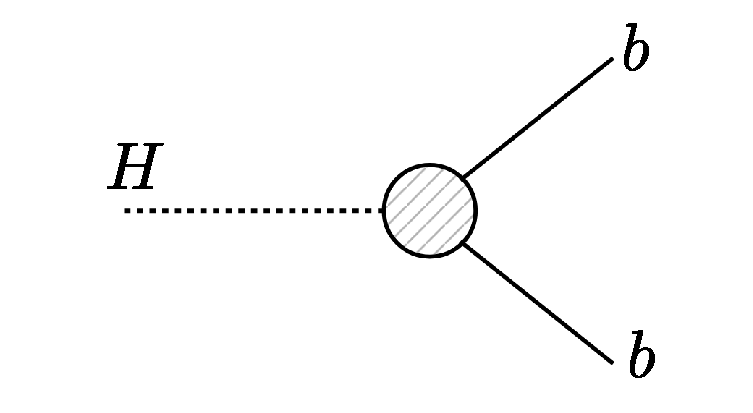
\includegraphics[width=2.5cm]{Figures/eft/eft_feynman/cd.pdf} \\

    $\mathcal{O}_\ell$ & $y_\ell|H|^2\bar{L}_LH^{\dagger}\ell_R + {\rm{h.c.}}$ & $c_\ell=-v^2\frac{w_\ell}{\Lambda^2}$ & H$\tau\tau$  & \vspace{.1cm}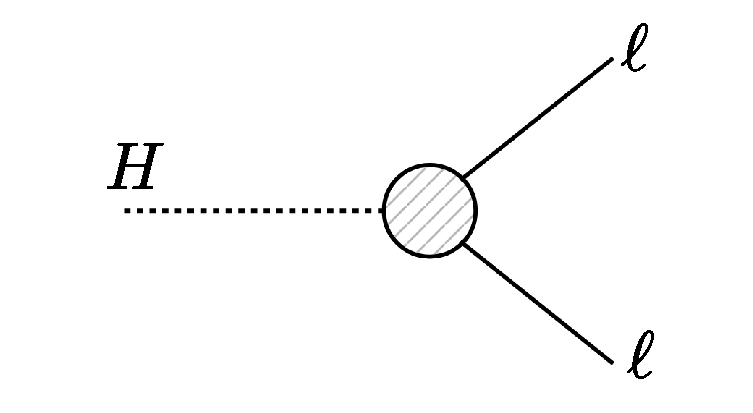
\includegraphics[width=2.5cm]{Figures/eft/eft_feynman/cl.pdf} \\

    $\mathcal{O}_{HW}$ & $i(D^\mu H)^{\dagger}\sigma^a(D^\nu H)W^a_{\mu\nu}$ & $c_{HW}=\frac{m_W^2}{2g}\frac{w_{HW}}{\Lambda^2}$ & HWW, HZZ  & \vspace{.1cm}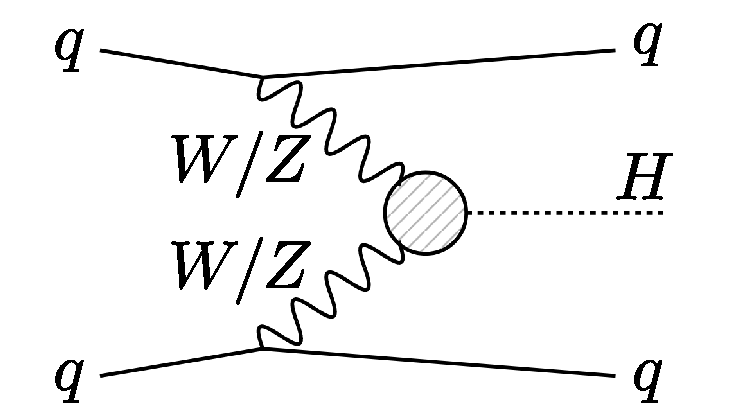
\includegraphics[width=2.5cm]{Figures/eft/eft_feynman/cHW.pdf} \\

    $\mathcal{O}_{WW}$ & $i(H^{\dagger}\sigma^aD^\mu H)D^\nu W^a_{\mu\nu}$ & $c_{WW}=\frac{m_W^2}{g}\frac{w_{WW}}{\Lambda^2}$ & HWW, HZZ & \vspace{.1cm}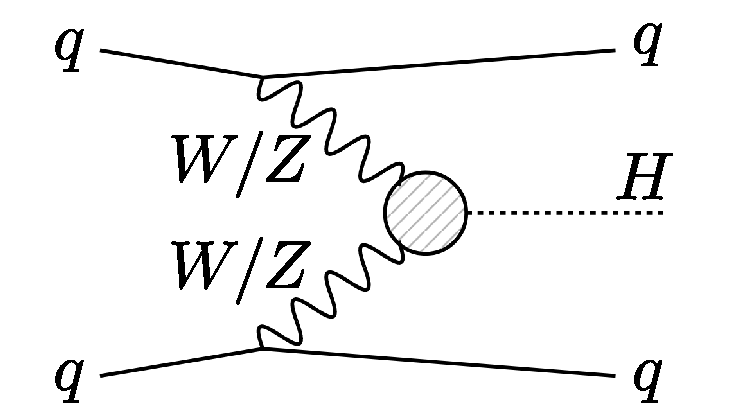
\includegraphics[width=2.5cm]{Figures/eft/eft_feynman/cHW.pdf} \\

    $\mathcal{O}_B$ & $i(H^{\dagger}D^\mu H)\partial^\nu B_{\mu\nu}$ & $c_{WW}=\frac{2m_W^2}{g'}\frac{w_{B}}{\Lambda^2}$ & HZZ & \vspace{.1cm}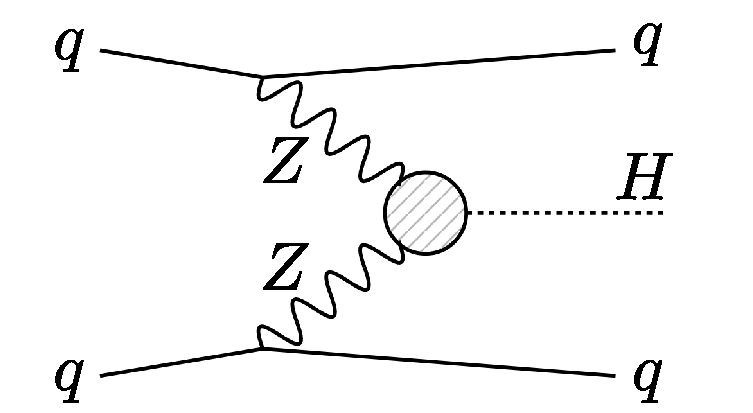
\includegraphics[width=2.5cm]{Figures/eft/eft_feynman/cB.pdf} \\

\end{tabular}
%   \hspace*{-.5cm}
\end{table}

\section{CMS Higgs combination}\label{sec:eft_combination}
The HEL interpretation is applied to the latest Higgs boson combination performed by the CMS experiment, documented in Ref.~\cite{CMS-PAS-HIG-19-005}. The combination includes analyses targeting all the major Higgs boson decay channels, with integrated luminosities ranging from 35.9~\fbinv to 137~\fbinv, depending on the input analysis. By targeting different final states, most analyses are orthogonal by construction. For similar final states, the overlap in the selected events has been checked and found to be negligible. 

The inclusion of different decay channels ensures sensitivity to a larger subset of operators (see Table~\ref{tab:hel_operators}). Each input analysis measures cross sections in the STXS framework, however, these measurements are performed using different STXS binning schemes with varying granularity.
Hence the EFT parametrisation of the signal yield is defined at the granularity of all binning schemes which enter the combination: stage 0, 1.0 and 1.1 (see Appendix~\ref{app:merging_schemes}). For stage 1.0 and above, the bins are split according to the event kinematics (e.g. \ptH, $N_{\rm{jets}}$ etc). As a result, the kinematic information available in these measurements helps to further constrain BSM effects beyond simple inclusive effects, and allows more directions in the parameter space to be probed simultaneously.

The full list of input analyses is provided in Table~\ref{tab:combination_inputs}. This combination was performed before the \Hgg analysis described in chapters~\ref{chap:hgg_overview}--\ref{chap:hgg_results}, and so the \Hgg inputs are taken from previous analyses. For each analysis, the targeted production modes and final states are listed, as well as the STXS stage of the measurements and the corresponding integrated luminosity. More detailed information on each input analysis can be found in the listed references.

\begin{table}[htb!]
  \centering
  \footnotesize
  \renewcommand{\arraystretch}{1.5}
  \setlength{\tabcolsep}{2pt}
  \caption[CMS Higgs boson combination input analyses]
  {
    Input analyses to the CMS Higgs boson combination, documented in Ref.~\cite{CMS-PAS-HIG-19-005}. The integrated luminosity used in each analysis is listed, as well as the targeted final states and production modes. No input analysis explicitly targets single-top associated production (tH). Also listed are the STXS binning schemes in which the measurements are performed. Despite entering the combination, the ggH \Hbb boosted analysis is left out of the EFT interpretation as the LO approximation of the EFT breaks down at very high $p_T^H$. Also, the \Hmumu measurements are not included as no branching fraction scaling function was available for the \Hmumu decay channel in Ref.~\cite{Hays:2673969}.
  }
  \label{tab:combination_inputs}
  \hspace*{-.7cm}
  \begin{tabular}{l|c|p{1cm}<{\centering}p{1cm}<{\centering}p{1cm}<{\centering}p{1cm}<{\centering}|c|c|c}
    \multirow{2}{*}{Decay channel} & \multirow{2}{*}{Final states} & \multicolumn{4}{c|}{Targeted production modes} & \multirow{2}{*}{STXS stage} & \multirow{2}{*}{$\mathcal{L}$~[\fbinv]} & \multirow{2}{*}{Ref.} \\ 
    & & ggH & qqH & VH lep & ttH & & & \\ \hline

    \multirow{2}{*}{\Hgg} & \multirow{2}{*}{$\gamma\gamma$} & X & X & - & - & 1.0 & 77.4 & \cite{CMS-PAS-HIG-18-029} \\
    & & - & - & - & X & 0 & 77.4 & \cite{Sirunyan:2018ouh,CMS-PAS-HIG-18-018} \\ \hline
    
    \Hfl & $4\mu$, $2e2\mu$, $4e$ & X & X & X & X & 1.1 & 137 & \cite{CMS-PAS-HIG-19-001} \\ \hline
    
    \HWW & \begin{tabular}{c}$e\mu$, $2e$, $2\mu$  \\ $e\mu+{\rm{jj}}$, $3\ell$, $4\ell$ \end{tabular} & X & X & X & - & 0 & 35.9 & \cite{Sirunyan:2018egh} \\ \hline
    
    \multirow{2}{*}{\Htautau} & \multirow{2}{*}{$e\mu$, $e\tau_h$, $\mu\tau_h$, $\tau_h\tau_h$} & X & X & - & - & 1.0 & 77.4 & \cite{CMS-PAS-HIG-18-032} \\
    & & - & - & X & - & 0 & 35.9 & \cite{Sirunyan:2018cpi} \\ \hline
    
    \multirow{3}{*}{\Hbb} & $\ell\ell+{\rm{bb}}$, $\ell\nu+{\rm{bb}}$, $\nu\nu+{\rm{bb}}$ & - & - & X & - & 0 & 77.4 & \cite{Sirunyan:2017elk,Sirunyan:2018kst} \\
    & \multirow{2}{*}{bb} & - & - & - & X & 0 & 77.4 & \cite{CMS-PAS-HIG-18-030} \\
    & & X & - & - & - & {\scriptsize{ggH high $p_T^H$}} & 35.9 & \cite{Sirunyan:2017dgc} \\ \hline
    
    ttH($\rightarrow$~leptons) & \begin{tabular}{c}$2\ell{\rm{ss}}$, $3\ell$, $4\ell$ \\ $1\ell+2\tau_h$,  $2\ell{\rm{ss}}+1\tau_h$, $3\ell+1\tau_h$\end{tabular} & - & - & - & X & 0 & 77.4 & \cite{Sirunyan:2018shy,CMS-PAS-HIG-18-019} \\ \hline
    
    \Hmumu & $\mu\mu$ & X & X & - & - & 0 & 35.9 & \cite{Sirunyan:2018hbu} \\
\end{tabular}
  \hspace*{-.7cm}
\end{table}

\subsection{Statistical procedure}
The statistical inference procedure used in the combination extends upon the procedure described in sections \ref{sec:category_likelihood} and \ref{sec:results_extraction}. A likelihood function\footnote{The dependence of the likelihood on the Higgs boson mass, $m_H$, has been dropped from the notation. For the form of the Poisson terms, please refer to equation \ref{eq:poisson_def}.} is constructed for each analysis category or \textit{region}, $k$, now defined for a generic final state, $f$,

\begin{equation}
    L_k({\rm{data}}\,|\,\vec{\alpha},\vec{\theta}_s,\vec{\theta_b}) = \mathcal{P}_k( {\rm{data}}\,|\,\vec{\alpha},\vec{\theta_s},\vec{\theta}_b),
\end{equation}

\noindent
where the quanta of the likelihood, $\mathcal{P}_k$, takes the following form for binned analysis regions,

\begin{equation}
    \mathcal{P}^{\rm{binned}}_k = \prod^{N_{\rm{bins}}}_X {\rm{Poisson}}\Big( N^{\rm{data}}_{k,X} \, \Big| \, \Big[\sum_{i,f} S^{i,f}_{k,X}(\vec{\alpha},\vec{\theta}_s) \Big] + B_{k,X}(\vec{\theta}_b) \Big).  
\end{equation}
\noindent
Here, the index $X$ runs over bins of some observable(s) e.g. \mgg for the \Hgg analyses. The quantity $S^{i,f}_{k,X}$ corresponds to the signal estimate in bin $X$, of analysis region $k$, originating from STXS bin, $i$, and decaying to final state, $f$. The background estimate and number of data events in the same observable bin are referred to as $B_{k,X}$ and $N^{\rm{data}}_{k,X}$, respectively. For unbinned analysis regions, the quanta is defined as,

\begin{equation}
    \mathcal{P}^{\rm{unbinned}}_k = \frac{1}{z} \prod^{z}_j {\rm{Poisson}}\Big(1 \, \Big| \, \Big[\sum_{i,f} S^{i,f}_{k}(\vec{\alpha},\vec{\theta}_s) \cdot \rho^{i,f}_{k,{\rm{sig}}}(x_j|\vec{\alpha},\vec{\theta}_s) \Big] + B_{k}(\vec{\theta}_b)\cdot \rho_{k,{\rm{bkg}}}(x_j|\vec{\theta}_b) \Big),
\end{equation}

\noindent
for $z$ events in data landing in region $k$, where each event is labelled by the index $j$. The terms $\rho^{i,f}_{k,{\rm{sig}}}(x)$ and $\rho_{k,{\rm{bkg}}}(x)$ are the probability density functions of some observable(s) $x$, for signal and background, respectively. The total signal and background yield estimates in region $k$ are expressed by $S^{i,f}_{k}$ and $B_{k}$. Comparing to the binned scenario, $S^{i,f}_{k}$ and $B_{k}$, are equal to the sum of the $S^{i,f}_{k,X}$ and $B_{k,X}$ terms over all observable bins, $X$. In all equations, it is assumed that the background estimate does not depend on the parameters of interest, $\vec{\alpha}$, which may not always be the case in a fully consistent EFT framework (see section \ref{sec:eft_improving}). Also, the modelling of the signal in terms of the observable(s) is extracted using the SM template, and is assumed to be independent of $\vec{\alpha}$: $\rho^{i,f}_{k,{\rm{sig}}}(x|\vec{\alpha},\vec{\theta})=\rho^{i,f}_{k,{\rm{sig}}}(x|\vec{\theta})$. For example, the shape of the signal \mgg peak in the \Hgg analysis is not parametrised as a function of the HEL parameters.

In the EFT interpretation, the signal yield for STXS bin, $i$, in final state, $f$, landing in analysis region, $k$ is expressed as, 

\begin{equation}\label{eq:signal_yield_eft}
    S_k^{i,f} = \mu^{i,f}(\vec{c}) \times \big[\sigma^i \cdot \mathcal{B}^{f} \big]_{\rm{SM}} \times \epsilon^{i,f}_k(\vec{c}) \times \mathcal{L}.
\end{equation}

\noindent
This is effectively an extension of equation \ref{eq:signal_yield}, where the explicit dependence on the HEL parameters, $\vec{c}\,(\equiv\vec{\alpha})$ is stated. The dependence on the nuisance parameters, $\vec{\theta}$, has been dropped from the notation for simplicity. The extraction of the cross section times branching fraction scaling functions, $\mu^{i,f}(\vec{c})$, is described in detail in section~\ref{sec:eft_parametrisation}. Interestingly, since the EFT operators can distort the event kinematics away from the SM hypothesis, the efficiency times acceptance values, $\epsilon^{i,f}_k(\vec{c})$ become dependent on the HEL parameters. This is especially true for measurements in the STXS framework, where the products of the Higgs boson decay are not restricted to fiducial phase space definitions. Nevertheless, in this interpretation, the so-called \textit{acceptance effects} are ignored,
\begin{equation}
   \epsilon^{i,f}_k(\vec{c})=\epsilon^{i,f}_k. 
\end{equation}
The potential impact of fully accounting for the detector efficiencies and analysis acceptance is investigated in section \ref{sec:eft_acceptance_corrections}.

The total likelihood is now defined as the product of the analysis region likelihood functions, taken over all input analyses included in the combination,

\begin{equation}
    L({\rm{data}}\,|\,\vec{\alpha},\vec{\theta}) = \prod_{k}^{N_{\rm{regions}}} \Big[    L_k({\rm{data}}\,|\,\vec{\alpha},\vec{\theta}) \,\Big] \times \mathcal{C}(\vec{\theta}) ,
\end{equation}

\noindent
where the constraint term, $\mathcal{C}$, takes the same form of that shown in section \ref{sec:category_likelihood}, such that deviations from the expected values of the nuisance parameters are penalised according to the associated prior. In the combination, the mass of the Higgs boson, $m_H$, is taken to be $m_H$~=~125.09~GeV. This represents the most precise measurement of $m_H$ at the time the combination was performed, determined from the combined LHC Run 1 ATLAS and CMS measurement, using the high resolution \Hgg and \Hfl decay channels~\cite{Aad:2015zhl}.

Since the different input analyses can have common sources of systematic uncertainty, the corresponding nuisance parameters must be correlated across decay channels. This follows the same procedure as described in section \ref{sec:correlation_scheme}, where in addition to defining per-year correlations, a single nuisance parameter is defined in the construction of the likelihood which affects the yield estimate in multiple decay channels simultaneously. 

All theoretical uncertainties arising from the renormalisation and factorisation scales used in the cross section calculations\footnote{This includes both the inclusive effects and the uncertainties modelling migrations \textit{across} STXS bins}, the parton distribution functions, and the branching fraction predictions are treated as fully correlated across decay channels. In addition, since other analyses use MC to estimate background contributions, it is necessary in these cases to introduce the uncertainties in the theoretical predictions of the background cross sections. These uncertainties are correlated between channels in which the same background appears. The results presented in this section are an \textit{interpretation} of cross section measurements, therefore the theory uncertainties directly affecting $[\sigma^i \cdot \mathcal{B}^{f}]_{\rm{SM}}$ (i.e. type $\vec{\theta}_s^{\rm{th}}$) are folded into the measurement.

Most experimental uncertainties are analysis specific (e.g. \mgg signal shape uncertainties), and are therefore uncorrelated. However, there are a number of exceptions. This includes the uncertainties in the luminosity estimates, the lepton efficiency scale factors, the jet energy scale and resolution, and the b tagging efficiency. For most channels, which do not use a specific treatment of the aforementioned uncertainty sources, they are treated as correlated nuisance parameters. More information regarding the experimental uncertainty correlation scheme is provided in Ref.~\cite{CMS-PAS-HIG-19-005}.

After the total likelihood function has been constructed, the method of extracting the final results is identical to that described in section \ref{sec:results_extraction}.

\subsection{Results in the signal strength parametrisation}
Figure \ref{fig:combination_mu} shows the results of the CMS Higgs boson combination using a signal strength parametrisation. An independent signal strength modifier, $\mu_i^f$, is introduced to scale each production mode, $i$, times decay channel, $f$. The observed correlations between the fitted signal strengths are displayed in Figure \ref{fig:combination_mu_corr}.

\begin{figure}[htb!]
  \centering
  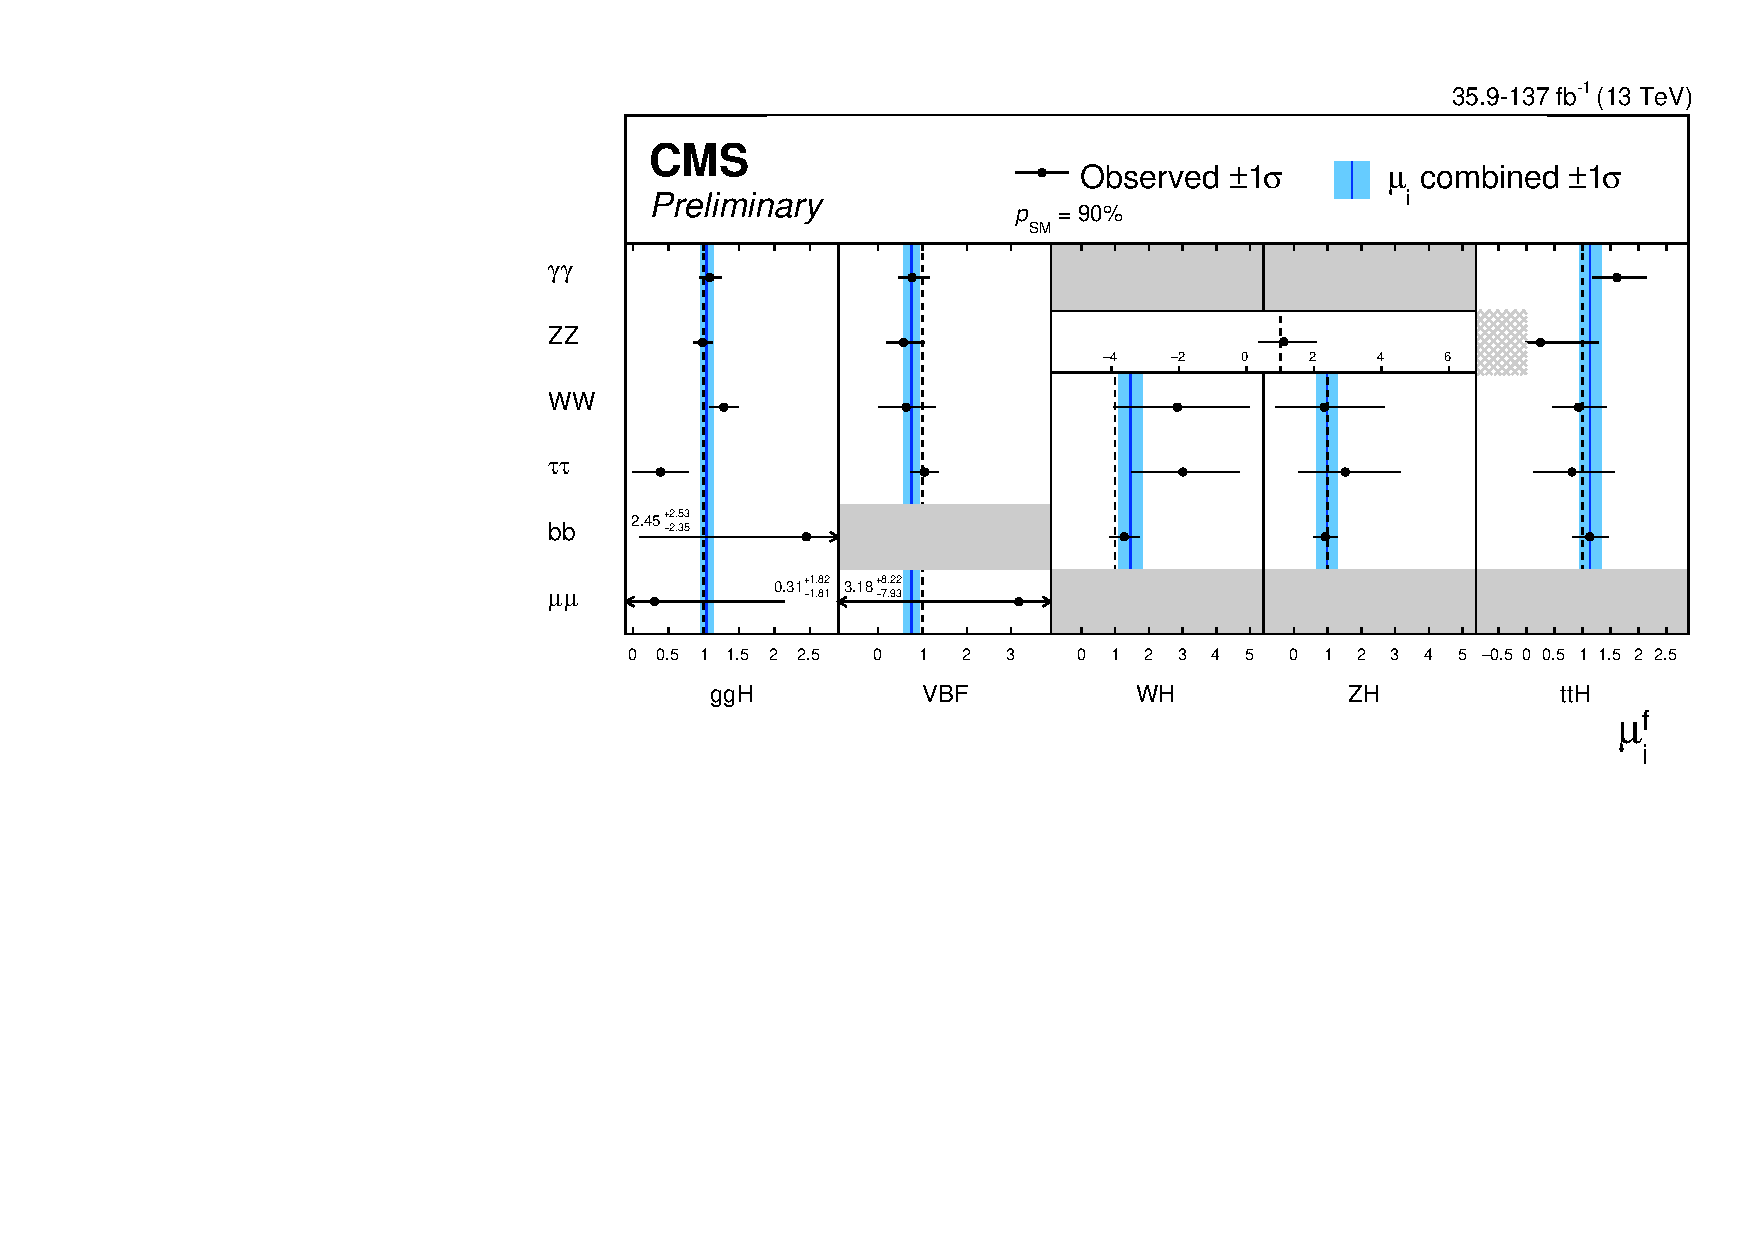
\includegraphics[width=1\textwidth]{Figures/eft/combination_mu.pdf}
  \caption[Results of the combination signal strength fit]
  {
    Observed best-fit values (black points) and 68\% confidence intervals (black lines) for the signal strength modifiers, $\mu_i^f$. The grey filled boxes indicate signal strength modifiers which are not included in the fit, since there is no input measurement targeting them. The hatched grey box indicates the restricted region in $\mu^{ZZ}_{ttH}$ for which the total signal plus background probability density function goes negative. For \HZZ, the WH and ZH production modes are fit together using a common signal strength modifier. This fit is extrememly compatible with the SM, with a corresponding $p$-value of approximately $p_{\rm{SM}}=90\%$. The blue bands indicate the results of a different parametrisation which introduces a per-production mode signal strength modifier, combined across decay channels. 
  }
  \label{fig:combination_mu}
\end{figure}

\begin{figure}[htb!]
  \centering
  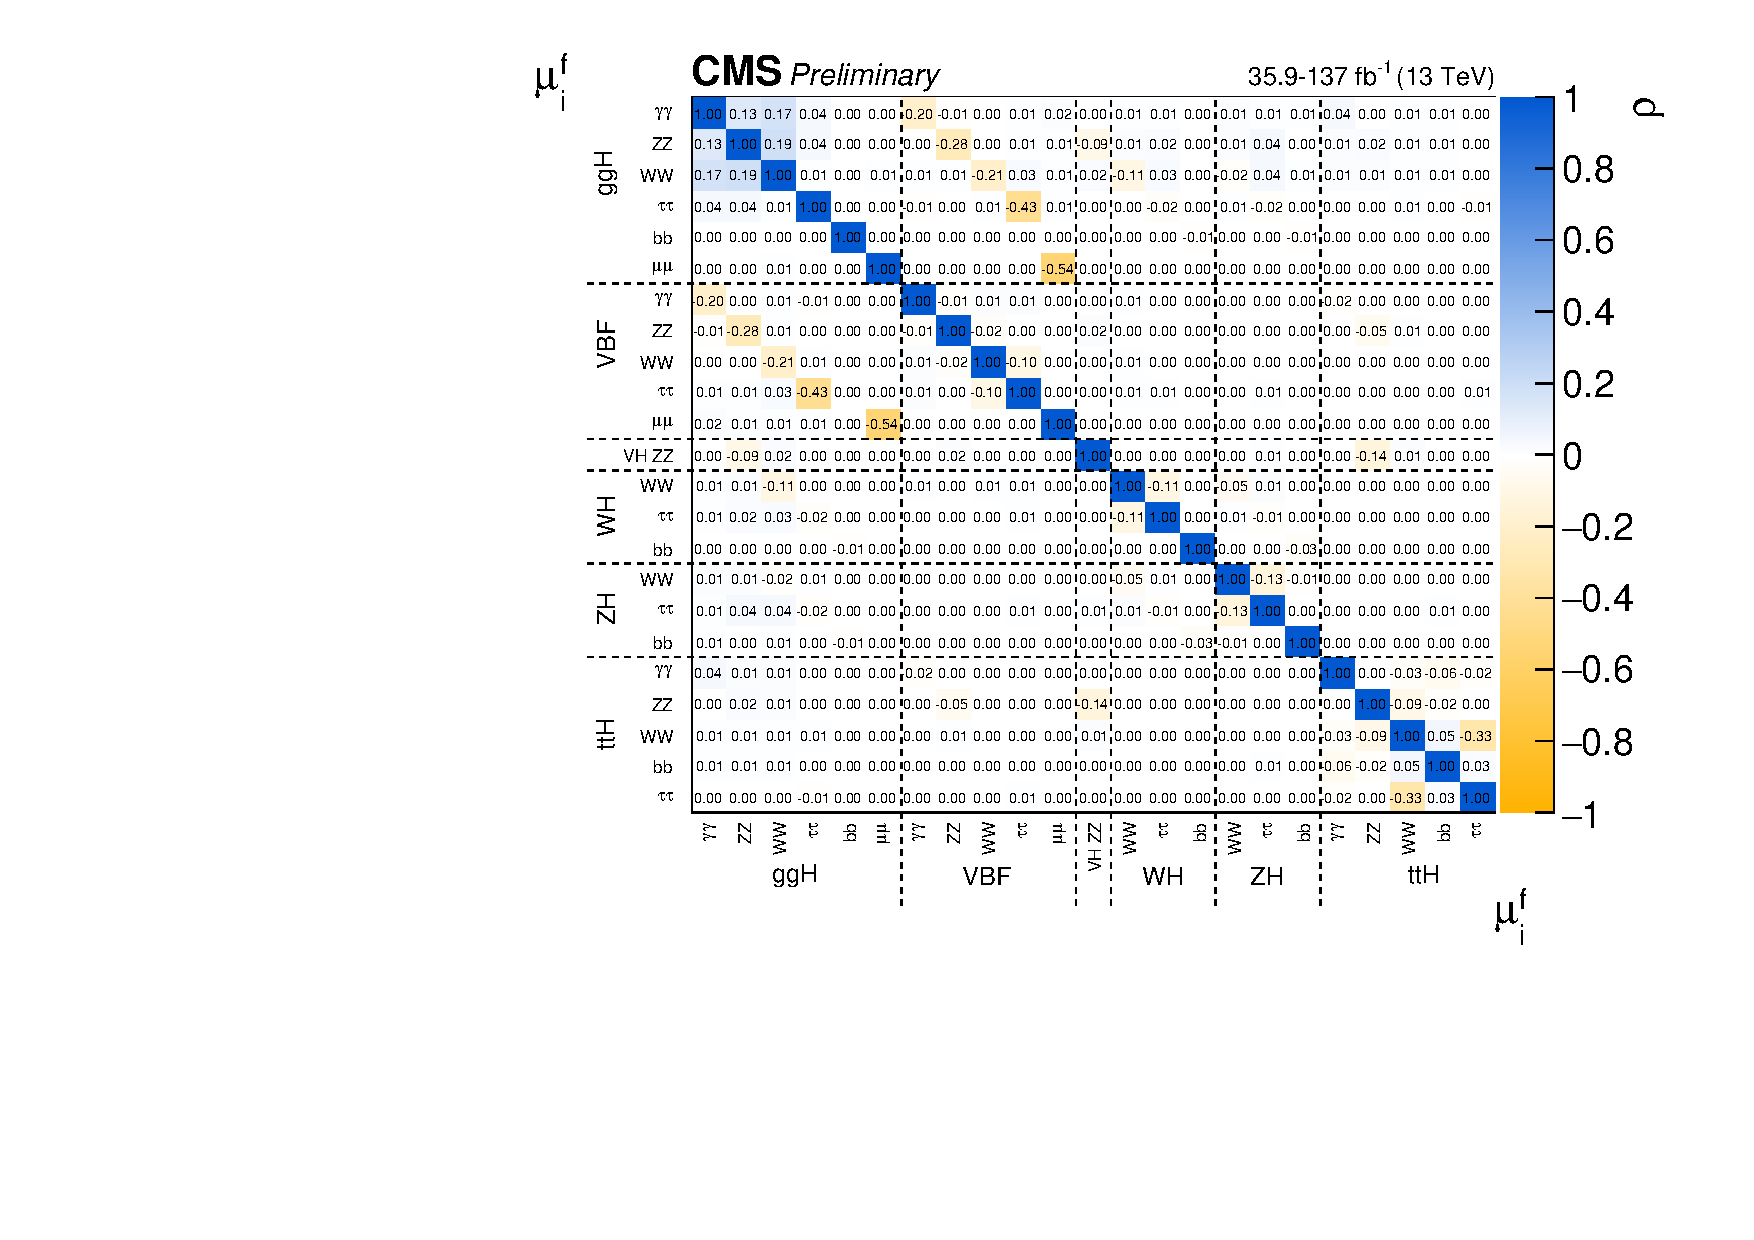
\includegraphics[width=1\textwidth]{Figures/eft/combination_mu_corr.pdf}
  \caption[Correlations in the combination signal strength fit]
  {
    Observed correlations between the fitted signal strengths. The size of the correlations is indicated by the colour scale.
  }
  \label{fig:combination_mu_corr}
\end{figure}

% \FloatBarrier
\section{Signal yield parametrization}\label{sec:eft_parametrisation}
The scaling functions, $\mu^{i,f}(\vec{c})$, shown in equation \ref{eq:signal_yield_eft}, parametrise the signal cross section times branching fractions as a function of HEL parameters, and are derived as follows. Within the HEL framework (equation \ref{eq:hel_expansion}) the amplitude for each Higgs boson production and decay process can be described as,

\begin{equation}\label{eq:hel_matrixelement}
    |\mathcal{M}_{\rm{HEL}}|^2 = \Big| \mathcal{M}_{\rm{SM}} + \mathcal{M}_{\rm{BSM}} \Big|^2 = |\mathcal{M}_{\rm{SM}}|^2 + 2{\rm{Re}}\{\mathcal{M}_{SM}\mathcal{M}^{\dagger}_{\rm{BSM}}\} + |\mathcal{M}_{\rm{BSM}}|^2,
\end{equation}

\noindent
where $\mathcal{M}_{\rm{SM}}$ and $\mathcal{M}_{\rm{BSM}}$ are the matrix elements originating from the SM and BSM parts of the Lagrangian, respectively. The total amplitude now contains an SM-BSM interference term, suppressed by a factor of $\Lambda^{-2}$, and a purely-BSM term, suppressed by a factor $\Lambda^{-4}$. In this interpretation, only one BSM vertex is considered per Feynman diagram, which means $\mathcal{M}_{\rm{BSM}}$ is linear in the HEL Wilson coefficients. Substituting this linearity condition into equation \ref{eq:hel_matrixelement}, and using the fact $\sigma \propto |\mathcal{M}|^2$, we arrive at an expression for the cross section of signal process, $i$,

\begin{equation}
    \sigma^i_{\rm{HEL}} = \sigma^i_{\rm{SM}} + \sigma^i_{\rm{int}} + \sigma^i_{\rm{BSM}},
\end{equation}

\noindent
resulting in a scaling function relative to the SM prediction which is quadratic in the HEL parameters,

\begin{equation}\label{eq:xs_scaling_functions}
    \mu^i_{\rm{prod}}(\vec{c}) = \frac{\sigma^i_{\rm{HEL}}}{\sigma^i_{\rm{SM}}} = 1 + \sum_p A^i_p\,c_p + \sum_{pr} B^i_{pr}\,c_p\,c_r,
\end{equation}

\noindent
where in this analysis, $i$, corresponds to the STXS bin. The terms, $A^i_p$ and $B^i_{pr}$, are constant prefactors which encode the impact of the HEL parameters on each STXS bin. We can ignore the $|\mathcal{M}_{\rm{BSM}}|^2$ term in the expansion simply by setting the $B^i_{pr}$ prefactors to zero. These terms, despite having an energy scale suppression of the same order as the leading dimension-8 SM-BSM interference contributions ($\Lambda^{-4}$), are kept in this interpretation since they are the leading purely-BSM terms and they prevent the scaling functions from going negative, thus leading to a better fit to data.

Applying the same reasoning, the partial Higgs boson decay width to final state $f$ scales relative to the SM prediction as,

\begin{equation}
    \frac{\Gamma^f_{\rm{HEL}}}{\Gamma^f_{\rm{SM}}} = 1 + \sum_p A^f_p\,c_p + \sum_{pr} B^f_{pr}\,c_p\,c_r.
\end{equation}

\noindent
It is necessary to also consider the variation in the total Higgs boson decay width, $\Gamma^H$, such that the scaling function of the branching fraction to final state f is expressed as,

\begin{equation}
    \mu^f_{\rm{decay}}(\vec{c}) = \frac{\mathcal{B}^f_{\rm{HEL}}}{\mathcal{B}^f_{\rm{SM}}} = \frac{\Gamma^f_{\rm{HEL}}/\Gamma^f_{\rm{SM}}}{\Gamma^H_{\rm{HEL}}/\Gamma^H_{\rm{SM}}} = \frac{1 + \sum\limits_p A^f_p\,c_p + \sum\limits_p \sum\limits_r B^f_{pr}\,c_p\,c_r}{1 + \sum\limits^{~}_p A^H_p\,c_p + \sum\limits_p \sum\limits_r B^H_{pr}\,c_p\,c_r}.
\end{equation}

The total scaling function for signal events originating from STXS bin, $i$, and decaying to final state, $f$, is the product of the individual cross section and branching fraction scaling functions,

\begin{equation}
    \mu^{i,f}(\vec{c}) = \mu^i_{\rm{prod}}(\vec{c}) \cdot \mu^f_{\rm{decay}}(\vec{c}).
\end{equation}

\noindent
This works under the narrow Higgs boson width assumption, such that the effects at production and decay have been factorised.

In summary, the Higgs boson signal scaling functions are uniquely described by the set of constant prefactors: $\{A^i_p,B^i_{pr},A^f_p,B^f_{pr},A^{H}_p,B^{H}_{pr}\}$. These prefactors are derived using LO MC samples with the reweighting procedure described in section \ref{sec:hel_derivation}. It should be stressed that the SM predictions for the cross sections and branching fraction in equation \ref{eq:signal_yield_eft} are computed at the highest available order, however the EFT parametrisation is derived using LO MC samples. This strategy therefore assumes that the corrections to the cross sections and branching fractions from HEL operators is comparable at LO and higher orders~\cite{Degrande:2016dqg}. Once defined, the scaling functions are then applied in the likelihood fit to extract the best-fit values and corresponding confidence intervals for the considered HEL parameters. 


\subsection{Derivation: Monte Carlo reweighting}\label{sec:hel_derivation}
The impact of the HEL operators is computed using the \texttt{HEL\_UFO} model~\cite{Alloul:2013naa} in Madgraph~\cite{Alwall:2014hca}, where the Higgs boson production and decay processes are generated at LO in both QCD and QED. The LO Madgraph reweighting functionality~\cite{Mattelaer:2016gcx} is utilised, to reweight the generated events to different points in the HEL parameter space, according to,

\begin{equation}
    W_{\vec{c}} = \frac{|\mathcal{M}^{\vec{c}}_{\rm{HEL}}|^2}{|\mathcal{M}^{\rm{nominal}}_{\rm{HEL}}|^2} \cdot W_{\rm{nominal}}
\end{equation}

\noindent
where $\mathcal{M}^{\vec{c}}_{\rm{HEL}}$ is the matrix element at the point in parameter space, $\vec{c}$, $\mathcal{M}^{\rm{nominal}}_{\rm{HEL}}$ is the matrix element at the nominal point, and $W_{\rm{nominal}}$ is the corresponding event weight at that nominal point. Here, the nominal point in parameter space is chosen as the SM: $\vec{c} = (0,0,...,0)$.

For each operator, $\mathcal{O}_p$, two weights are defined by setting $c_p$ to two different values ($a$,$2a$), whilst all other HEL parameters are kept at 0. In doing so, simultaneous equations are constructed, as shown in \ref{eq:HEL_simultaneous}, where the reweighted and SM values of the observable, $X$ ($\sigma^i$ for production, $\Gamma^f$ for decay), can be used to infer the values of $A_p$ and $B_{pp}$,

\begin{equation}\label{eq:HEL_simultaneous}
    \begin{split}
        \frac{X_{c_p=a}}{X_{\rm{nominal}}} = 1 + a \cdot A_p + a^2 \cdot B_{pp} \\
        \frac{X_{c_p=2a}}{X_{\rm{nominal}}} = 1 + 2a \cdot A_p + 4a^2 \cdot B_{pp}.
    \end{split}
\end{equation}

\noindent
An additional weight is required to extract the cross-terms, $B_{pr}$ where $p \neq r$. This is defined by setting $(c_p,c_r)=(a,a)$, and keeping all other HEL parameters at 0, such that,

\begin{equation}
    \frac{X_{(c_p,c_r)=(a,a)}}{X_{\rm{nominal}}} = 1 + a \cdot (A_p+A_r) + a^2 \cdot (B_{pp}+B_{rr}+B_{pr}).
\end{equation}

\noindent
The value of $B_{pr}$ can then be inferred by using the previously calculated prefactors, $\{A_p,A_r,B_{pp},B_{rr}\}$, from equation \ref{eq:HEL_simultaneous}. In total, the number of weights required to fully specify the scaling functions is,

\begin{equation}
    N_{\rm{weights}} = 1 + 2N + \frac{N(N-1)}{2},
\end{equation}

\noindent
where $N$ is the number of operators; this analysis considers 8 HEL operators and therefore requires 45 weights, including the nominal SM weight. The value of $a$ is chosen to be small (0.01) to ensure the EFT effects do not blow up in the matrix element calculations, and therefore do not invoke a large statistical uncertainty in the calculated prefactors.

No additional generator-level kinematic cuts are applied except the default ones in Madgraph. All events are interfaced with \textsc{Pythia8} for parton showering and hadronisation~\cite{Sjostrand:2014zea}. A matching is performed using the \texttt{MLM} algorithm~\cite{Alwall:2007fs} to remove phase space overlap between jets specified in the matrix element and those originating from the parton shower.

The generator option choices used in the event simulation can affect the values of the prefactors, and therefore the scaling functions. For example, the EFT effects originate solely from the matrix element (in Madgraph) and not from the parton showering (in \textsc{Pythia8}). As a result, the values of the prefactors can depend on the scheme and parameters used for the jet matching. In general, these generator options have a small effect on the final parametrisation. Nevertheless it is important to specify the options used when reporting results; a summary of the MC options used in this interpretation is provided in Appendix~\ref{app:generator_options}.

\subsection{Effect at production}
Each Higgs boson production mode is generated separately, according to the Madgraph process definitions listed in Appendix~\ref{app:generator_options}. The Higgs boson decay is not specified in the process definition, such that EFT effects only enter in the Higgs boson production interaction vertices. The option \texttt{NP<=1} limits the number of BSM vertices to one per Feynman diagram. After interfacing with \textsc{Pythia8}, the particle-level events are propagated through the Rivet program~\cite{Buckley:2010ar}, using the \texttt{HiggsTemplateCrossSections} routine. This routine sequentially extracts the simulated event constituents, forms hadronic jets with the \textsc{FastJet} packagage~\cite{Cacciari:2011ma} using the anti-$k_T$ algorithm with a distance parameter of 0.4~\cite{Cacciari:2008gp}, calculates high-level kinematic quantities (e.g. \ptH, \ptV, \ptHjj, \mjj, $N_{\rm{jets}}$) and, finally, \textit{classifies} the simulated events according to their truth-level STXS bin. In all steps including the classification, the Higgs boson decay products formed by \textsc{Pythia8} are neglected. The routine has been modified to output the bin classification at each stage of the STXS framework considered in the combination: stage 0, 1.0 and 1.1.

\begin{figure}[htb!]
  \centering
  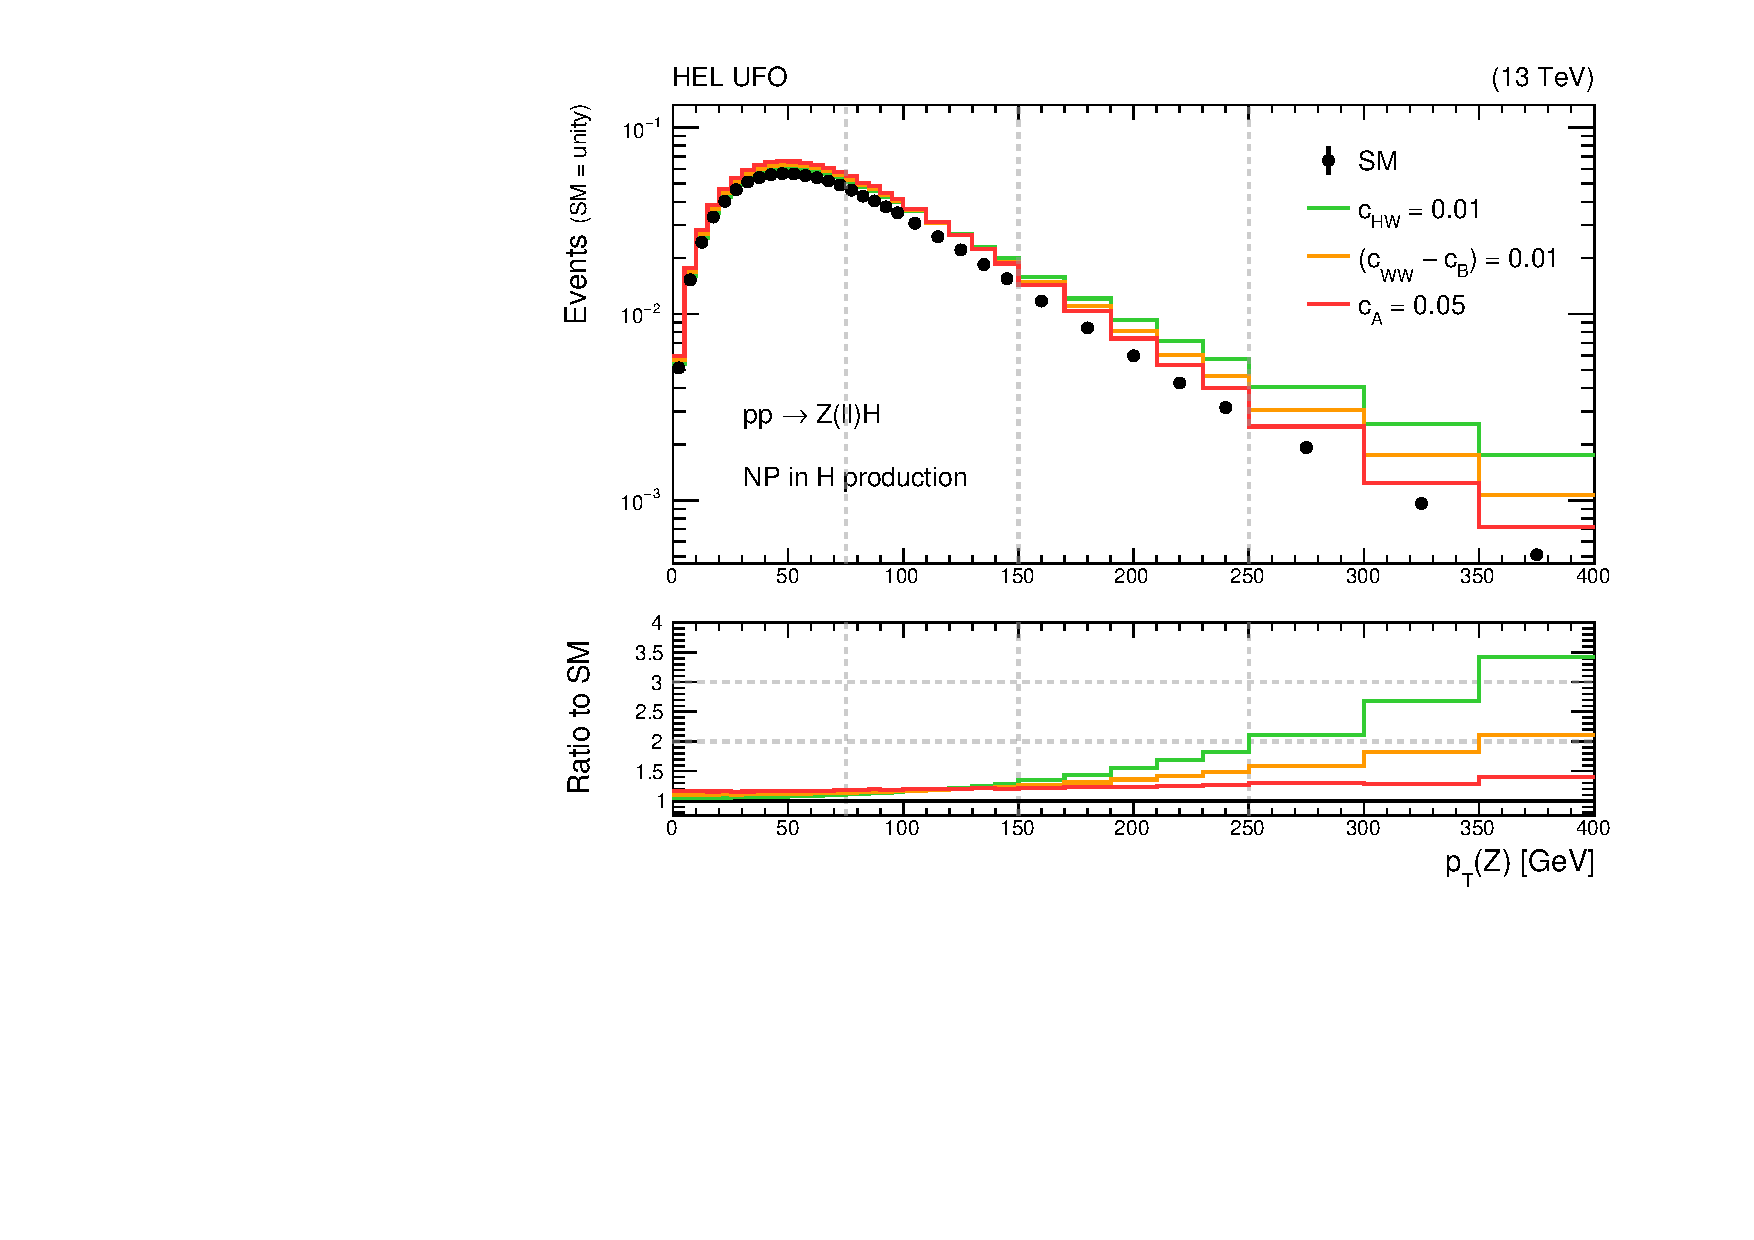
\includegraphics[width=.8\textwidth]{Figures/eft/distributions/HEL_PTZ.pdf}
  \caption[Transverse momentum of Z boson for ZH lep events with HEL contributions]
  {
    The Z boson transverse momentum, $p_T^Z$, spectrum for ZH lep events generated at LO. The black points correspond to the SM prediction, whilst the coloured lines show the distribution when various EFT contributions are introduced.
  }
  \label{fig:zhlep_ptv}
\end{figure}

A large number of events are generated for each production mode ($10^6$) to ensure each STXS bin is sufficiently populated. As a result the uncertainty in the scaling function prefactors arising from the limited MC statistics is small (typically below 1\%). The set of 45 event weights are then applied to extract the SM and EFT reweighted cross sections of each individual STXS bin, which are subsequently used to calculate the relevant prefactors: $\{A^i_p,B^i_{pr}\}$, according to the prescription described above. 


Figure \ref{fig:zhlep_ptv} shows the $p_T^Z$ distribution for ZH lep events in the SM (black points) and when turning on various HEL parameters (coloured lines). The enhancement due to the $c_{HW}$ and $c_{WW}-c_B$ parameters grows with increasing $p_T^Z$; improving the measurements of this high $p_T$ region of phase space would allow for tighter constraints on these parameters. The dashed lines in the plot indicate the boundaries in $p_T^Z$ which define the ZH lep STXS stage 1.1 bins\footnote{In addition, the ZH lep $150<\ptV<250$~GeV region is further split into bins with zero jets and at least one jet}. The cross section scaling functions, $\mu_{\rm{prod}}^i(\vec{c})$, for each of these bins are shown as a function of $c_{HW}$ and $c_{WW}-c_B$ in Figure \ref{fig:zhlep_sf_1d}. In the plots, all other HEL parameters apart from the dependent variable are set to zero. Clearly the dependence on the HEL parameters increases as a function of $p_T^Z$. Going further, Figure \ref{fig:zhlep_sf_2d}, shows $\mu_{\rm{prod}}^i(\vec{c})$ for the ZH lep STXS stage 0 bin, considering variations in the pair of HEL parameters: $(c_{WW}-c_B)$ and $c_{HW}$. The tilt in the distribution arises from the relevant cross-term, $B_{WW-B,HW}$.

\begin{figure}[htb!]
  \centering
  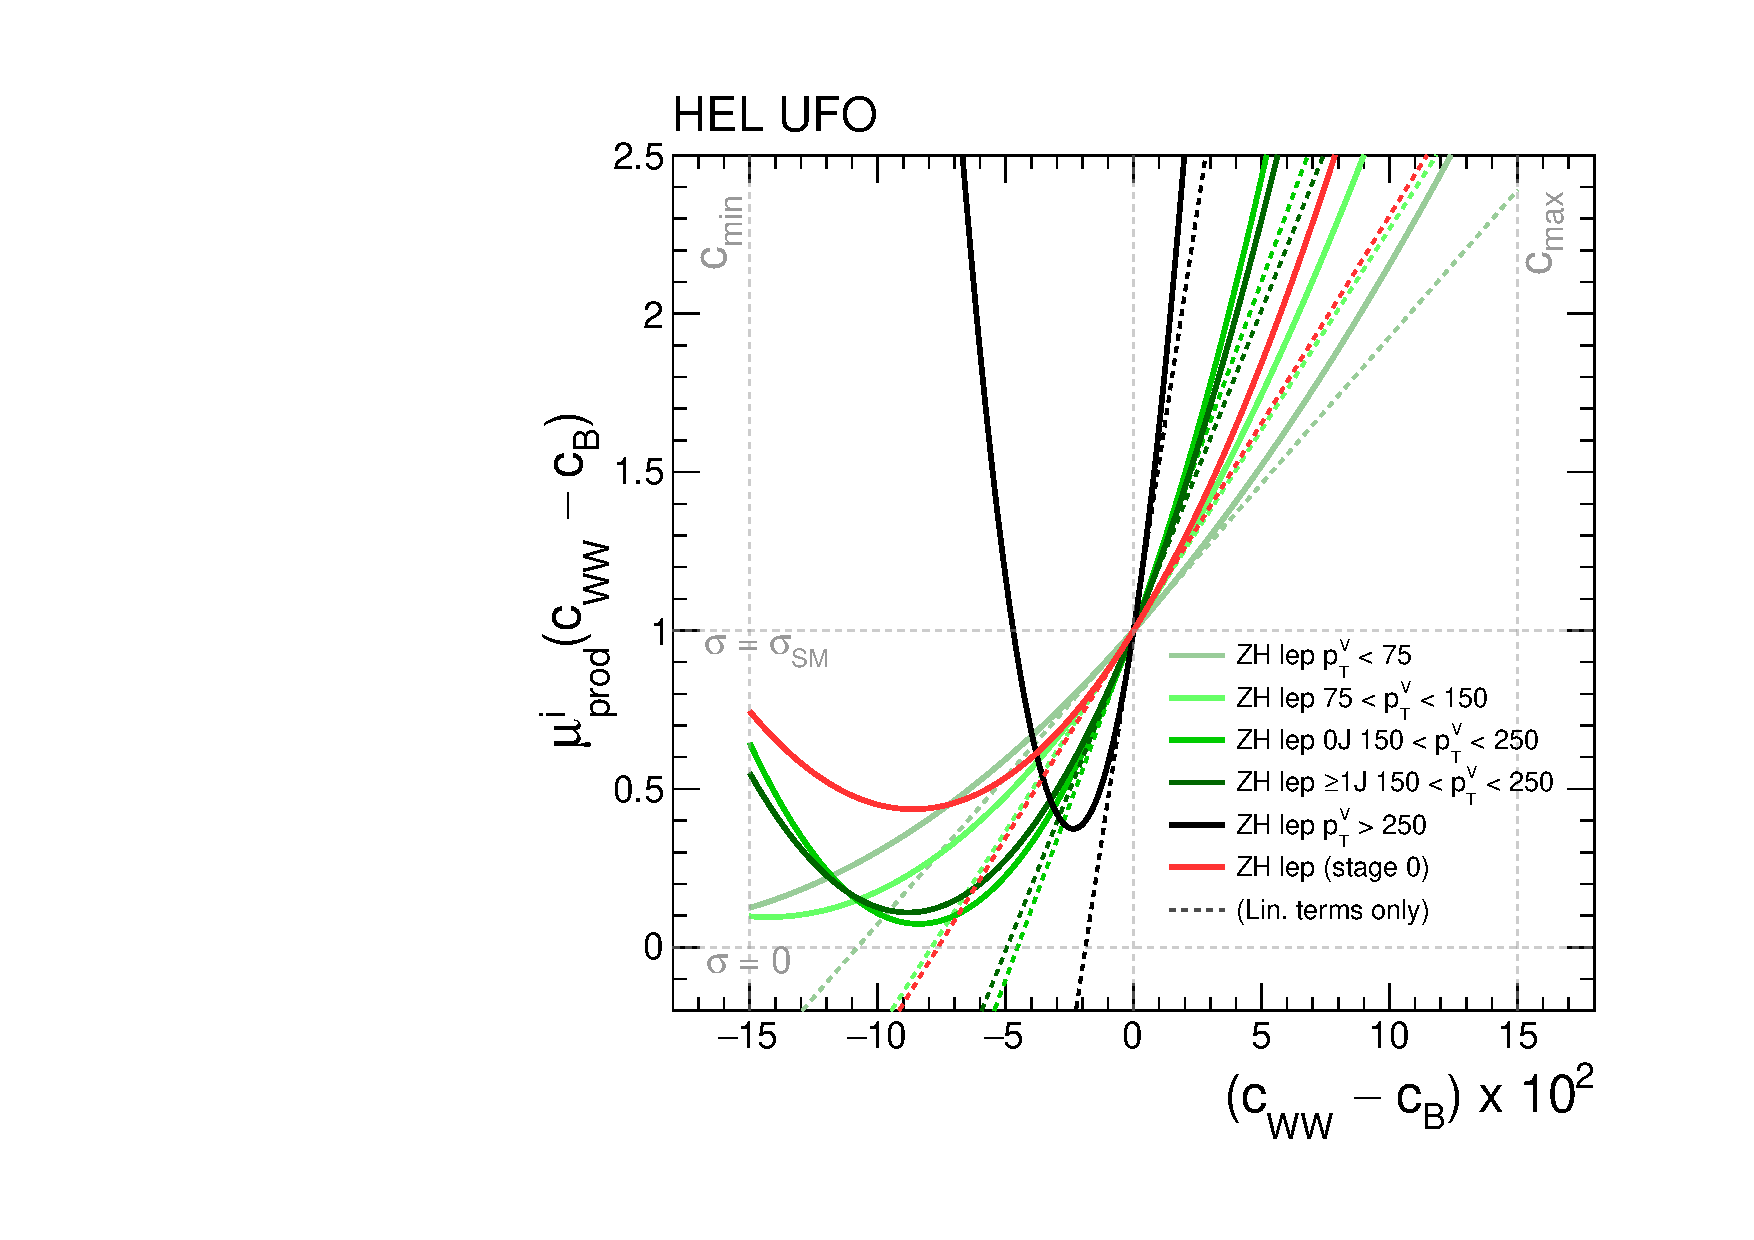
\includegraphics[width=.48\textwidth]{Figures/eft/scaling_functions/ZH_lep_vs_cWWMinuscB.pdf}
  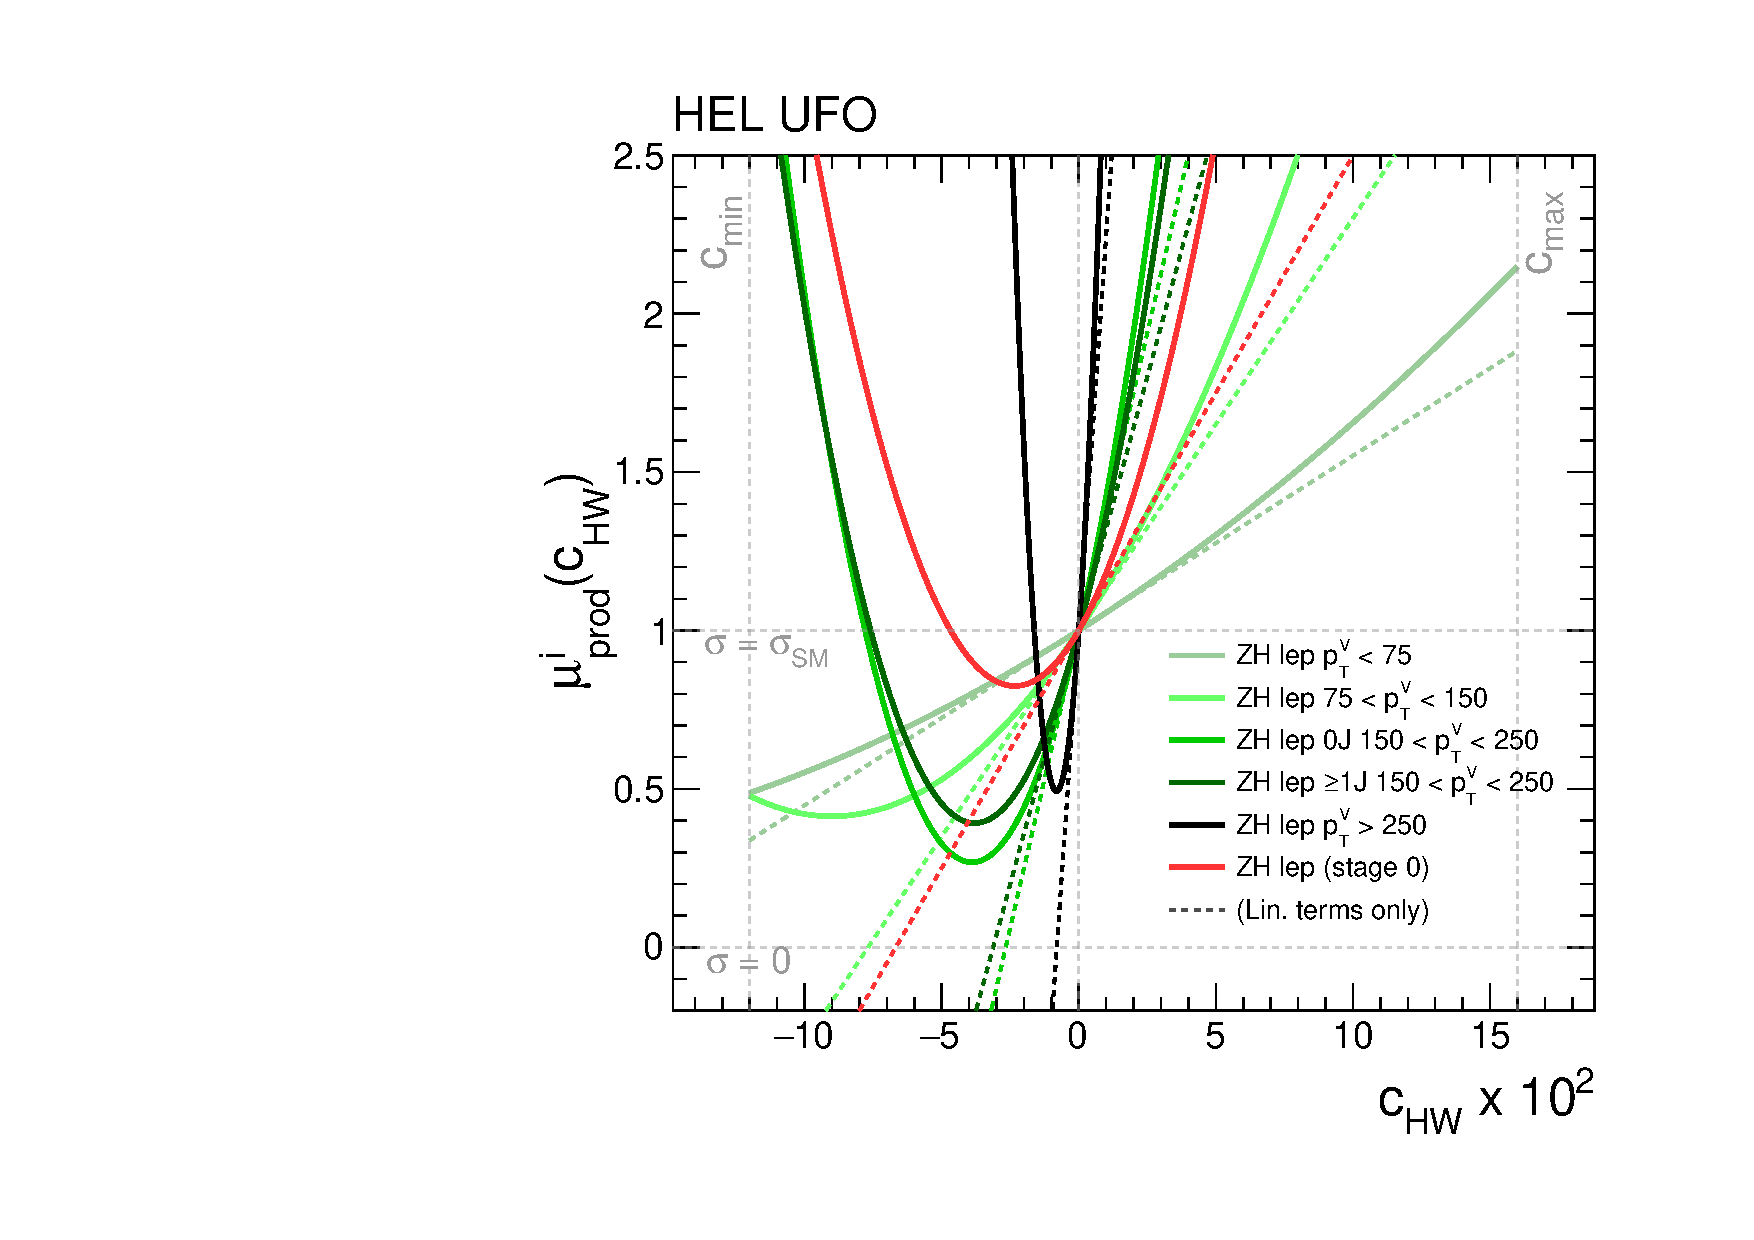
\includegraphics[width=.48\textwidth]{Figures/eft/scaling_functions/ZH_lep_vs_cHW.pdf}
  \caption[HEL cross section scaling functions for ZH leptonic STXS stage 1.1 bins]
  {
    Cross section scaling functions, $\mu_{\rm{prod}}^i(\vec{c})$, for the ZH leptonic STXS stage 1.1 bins in terms of $c_{WW}-c_B$ (left) and $c_{HW}$ (right). The red line shows the scaling behaviour for inclusive ZH leptonic production (stage 0). The dashed lines indicate the scaling functions when only the linear terms are considered ($B_{pr}=0$).
  }
  \label{fig:zhlep_sf_1d}
\end{figure}

\begin{figure}[htb!]
  \centering
  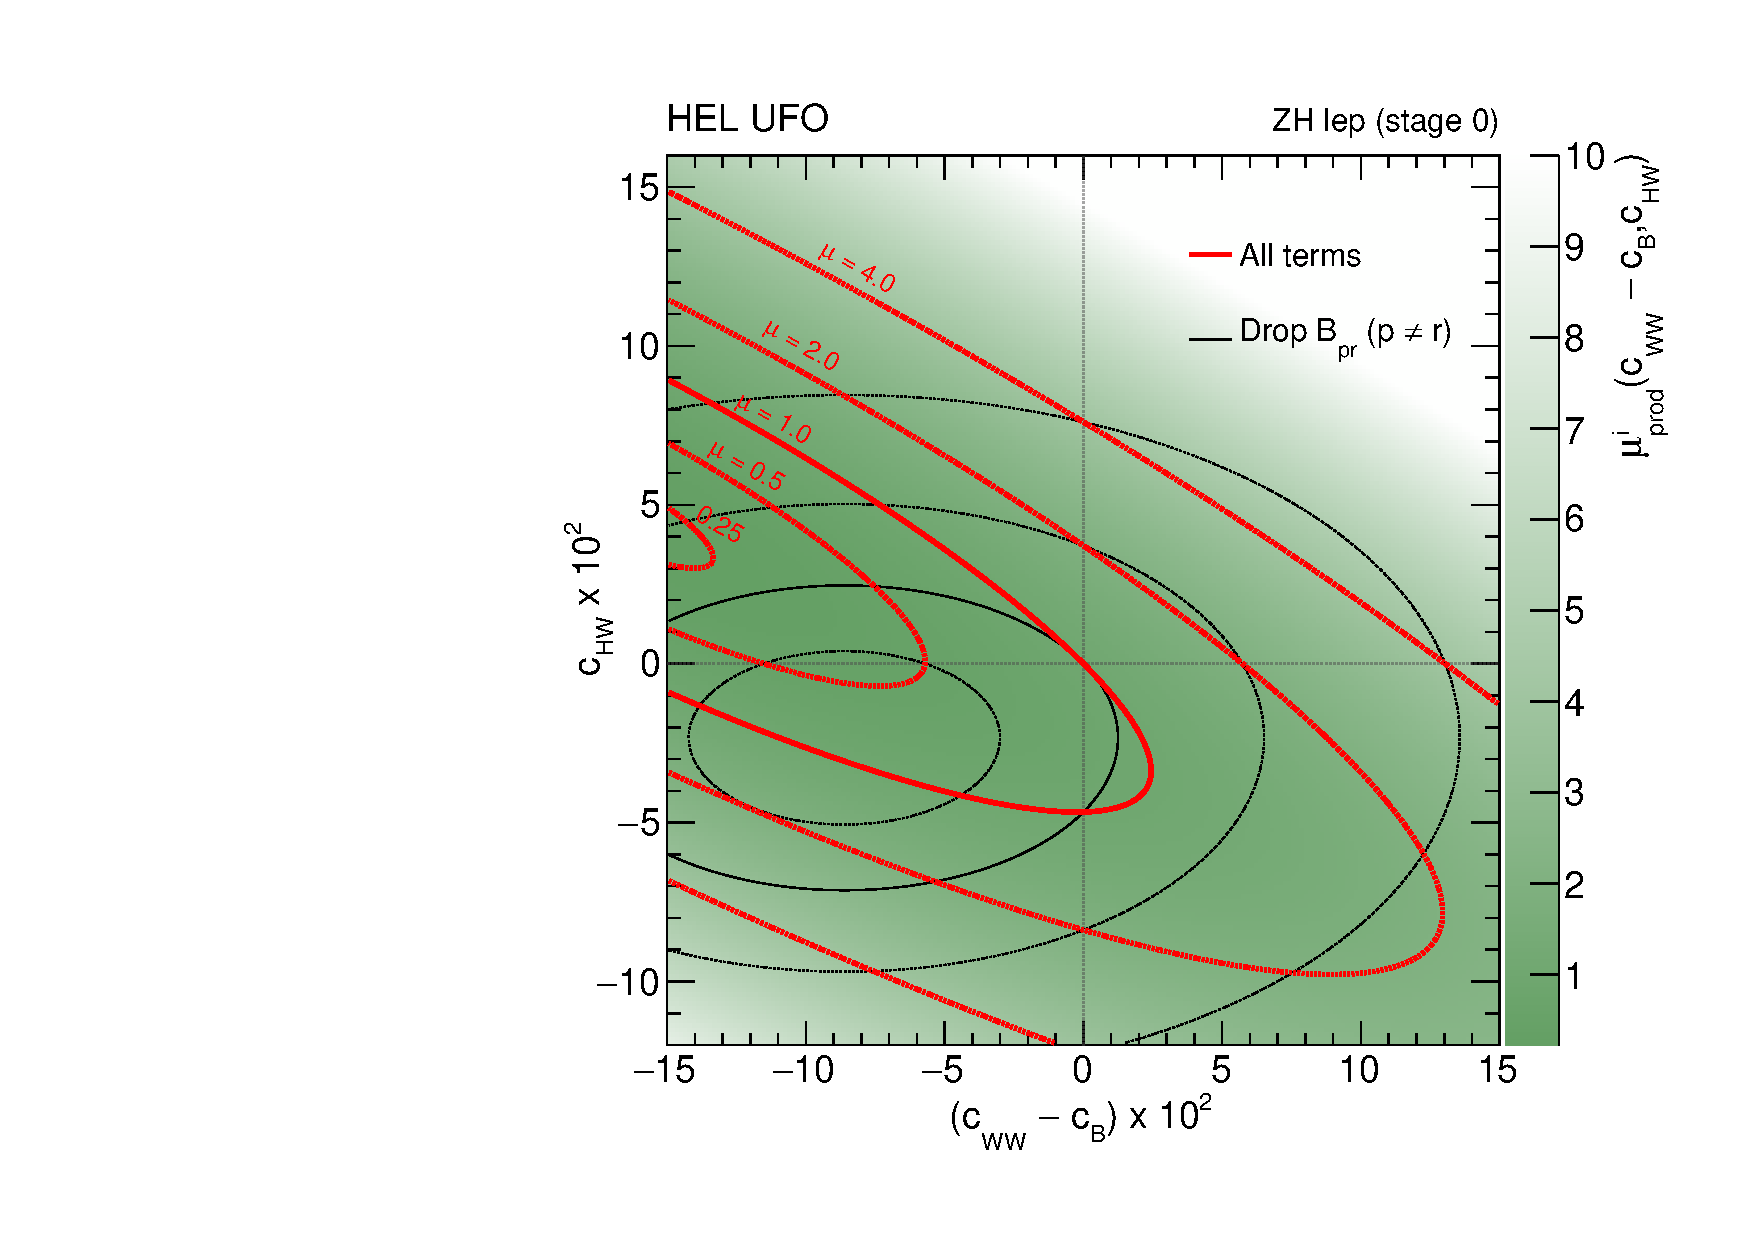
\includegraphics[width=.7\textwidth]{Figures/eft/scaling_functions/ZH_lep_cWWMinuscB_vs_cHW.pdf}
  \caption[Two-dimensional HEL cross section scaling function for ZH lep STXS stage 0 bin]
  {
    Cross section scaling function, $\mu_{\rm{prod}}^i(\vec{c})$, for inclusive ZH leptonic production (stage 0), considering variations in the pair of HEL parameters: $(c_{WW}-c_B)$ and $c_{HW}$. The contours indicate lines of constant $\mu$. The black lines show the scaling function when the cross-term, $B_{WW-B,HW}$, is neglected.
  }
  \label{fig:zhlep_sf_2d}
\end{figure}

The scaling functions for the inclusive ttH STXS bin\footnote{The ttH production mode is only split (according to $p_T^H$) at stage 1.2.} is shown as a function of $c_u$ in Figure \ref{fig:tth_sf_1d}. Interestingly, the scaling function is equal to unity for two distinct values of $c_u$ within the allowed range of the parameter: at the SM point ($c_u=0$) and at $c_u=-4/3$. Without additional measurements sensitive to $c_u$ entering the likelihood, it is impossible to distinguish between these two points in parameter space. As a result the $q(c_u)$ likelihood curve from the results extraction will exhibit a double minimum structure, with minima situated around $c_u=0$ and $c_u=-4/3$. The inclusion of the tH production cross section measurement shown in chapter \ref{chap:hgg_results} would help alleviate this degeneracy. A similar degeneracy is observed in the ZH lep scaling functions in Figure~\ref{fig:zhlep_sf_1d}. This, however, is broken by including other measurements in the combination which depend different on $c_{HW}$ and $(c_{WW}-c_B)$: the qqH and WH lep production modes, and the \HZZ and \HWW decay channels.

\begin{figure}[htb!]
  \centering
  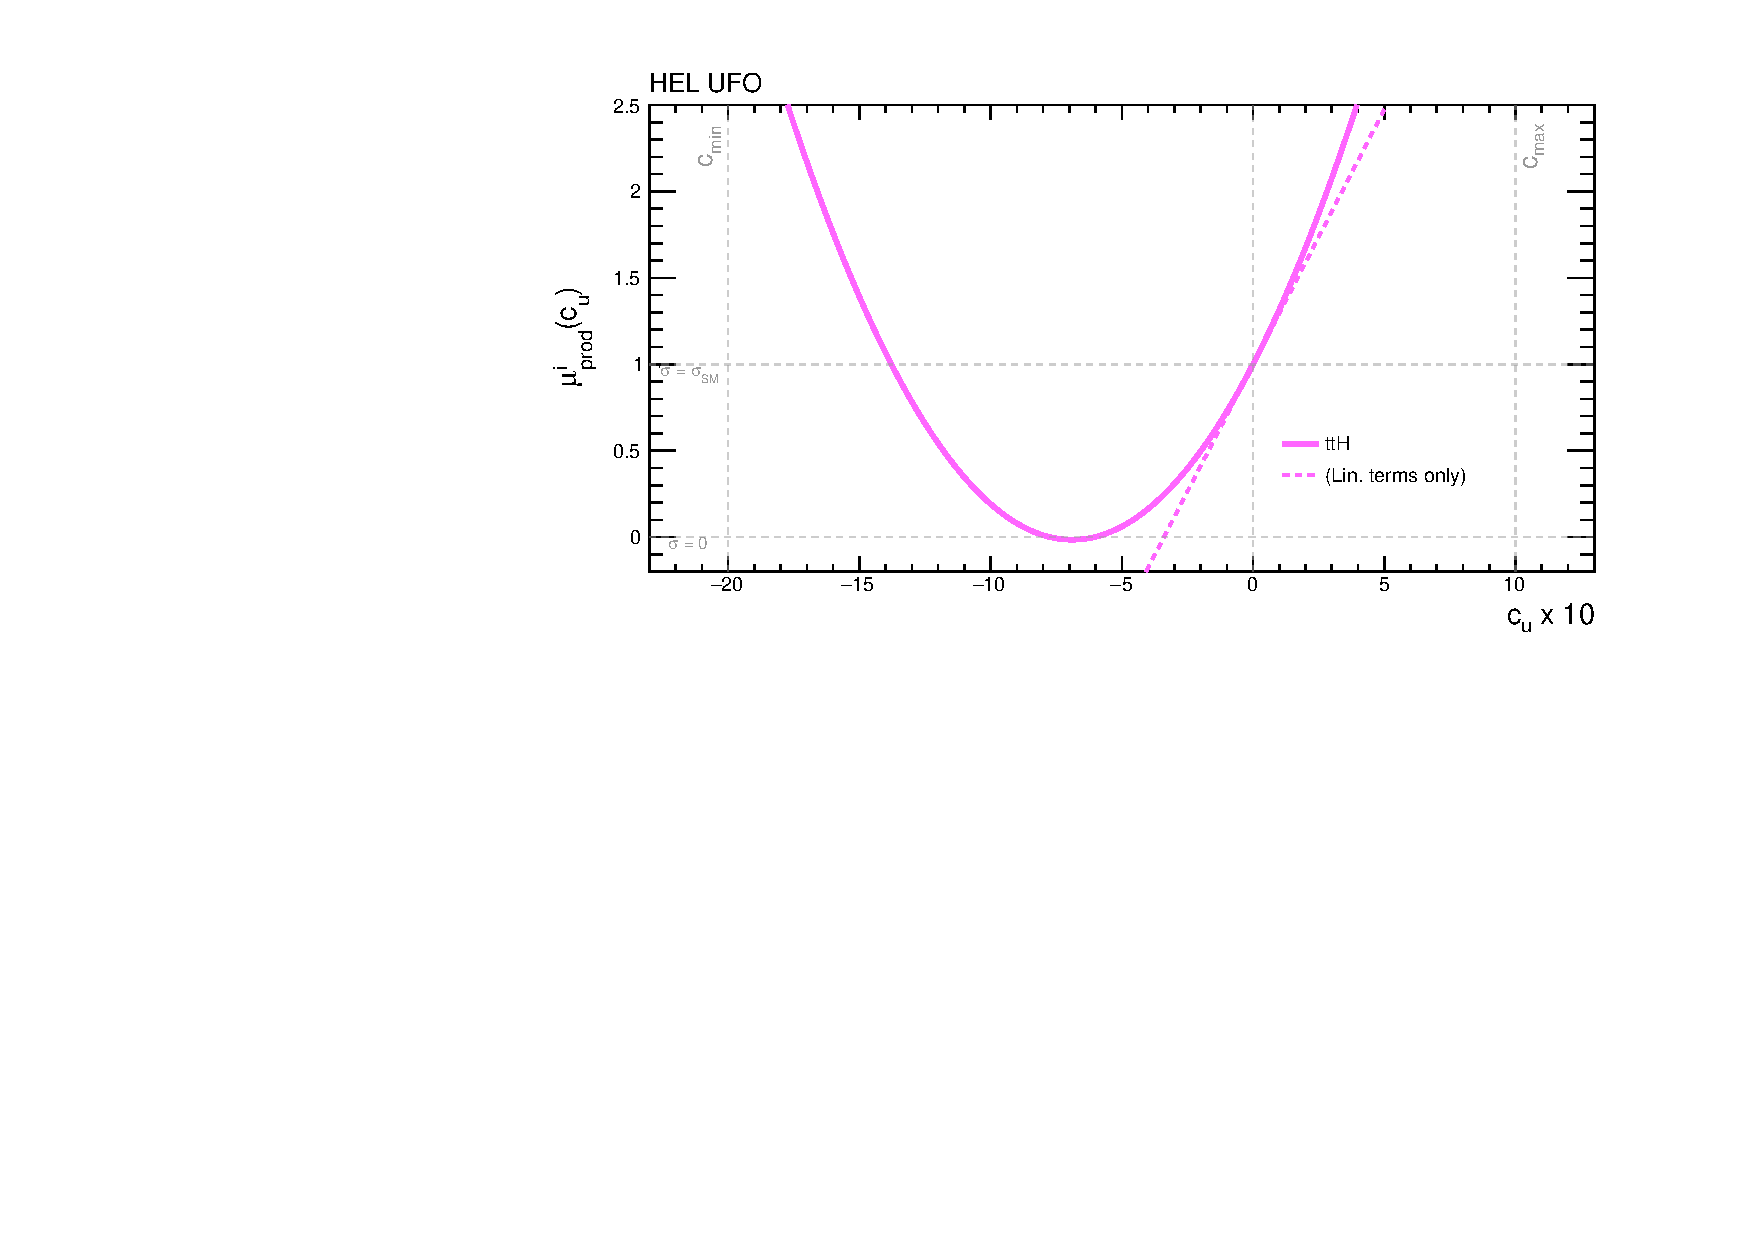
\includegraphics[width=.7\textwidth]{Figures/eft/scaling_functions/ttH_vs_cu.pdf}
  \caption[HEL cross section scaling function for ttH STXS bin]
  {
    Cross section scaling functions, $\mu_{\rm{prod}}^i(\vec{c})$, for ttH production in terms of $c_{u}$. The dashed line indicates the scaling function when only the linear term are considered ($B_{uu}=0$).
  }
  \label{fig:tth_sf_1d}
\end{figure}


\subsection{Effect at decay}
The decay mode parametrisation is taken directly from Ref.~\cite{Hays:2673969}. Higgs bosons are generated at rest and are made to decay in a particular channel (see Appendix~\ref{app:generator_options}), where the EFT effects enter the Higgs boson decay vertices. The STXS framework does not include a fiducial region definition for the Higgs boson decay products, and therefore the EFT effects at decay are defined for the inclusive Higgs boson decay phase space. 

%If the acceptance effects were considered ($\epsilon^{i,f}_k(\vec{c})$), it would be necessary to generate the Higgs boson with a non-zero momentum spectrum to correctly describe the phase space of the decay products. 

The partial width scaling functions are derived using a similar approach to the cross section scaling functions. This amounts to extracting the SM prediction of the partial width at LO and the partial width with EFT effects turned on, and following the derivation procedure outlined in section \ref{sec:hel_derivation}. The total Higgs boson decay width parametrisation is then inferred from the sum of all partial width scaling functions, where the decay channels are weighted in the sum according to their total contribution to $\Gamma^{H}$. Figure \ref{fig:eft_decay} summarises the branching fraction scaling functions, $\mu_{\rm{decay}}^f(\vec{c})$, for the decay channels considered in the CMS Higgs boson combination. As the \Hbb decay channel has the largest branching fraction, the greatest impact on the total decay width is from the $c_d$ parameter. Also, in accordance with ttH production, the \Hbb and \Htautau scaling functions have two points in $c_d$ and $c_\ell$ respectively, which correspond to the SM prediction (unity). Again, since no additional measurements are included in the combination which are sensitive to these parameters, the corresponding $q(c_d)$ and $q(c_\ell)$ likelihood curves will exhibit a double-minimum structure.

\begin{figure}[htb!]
  \centering
  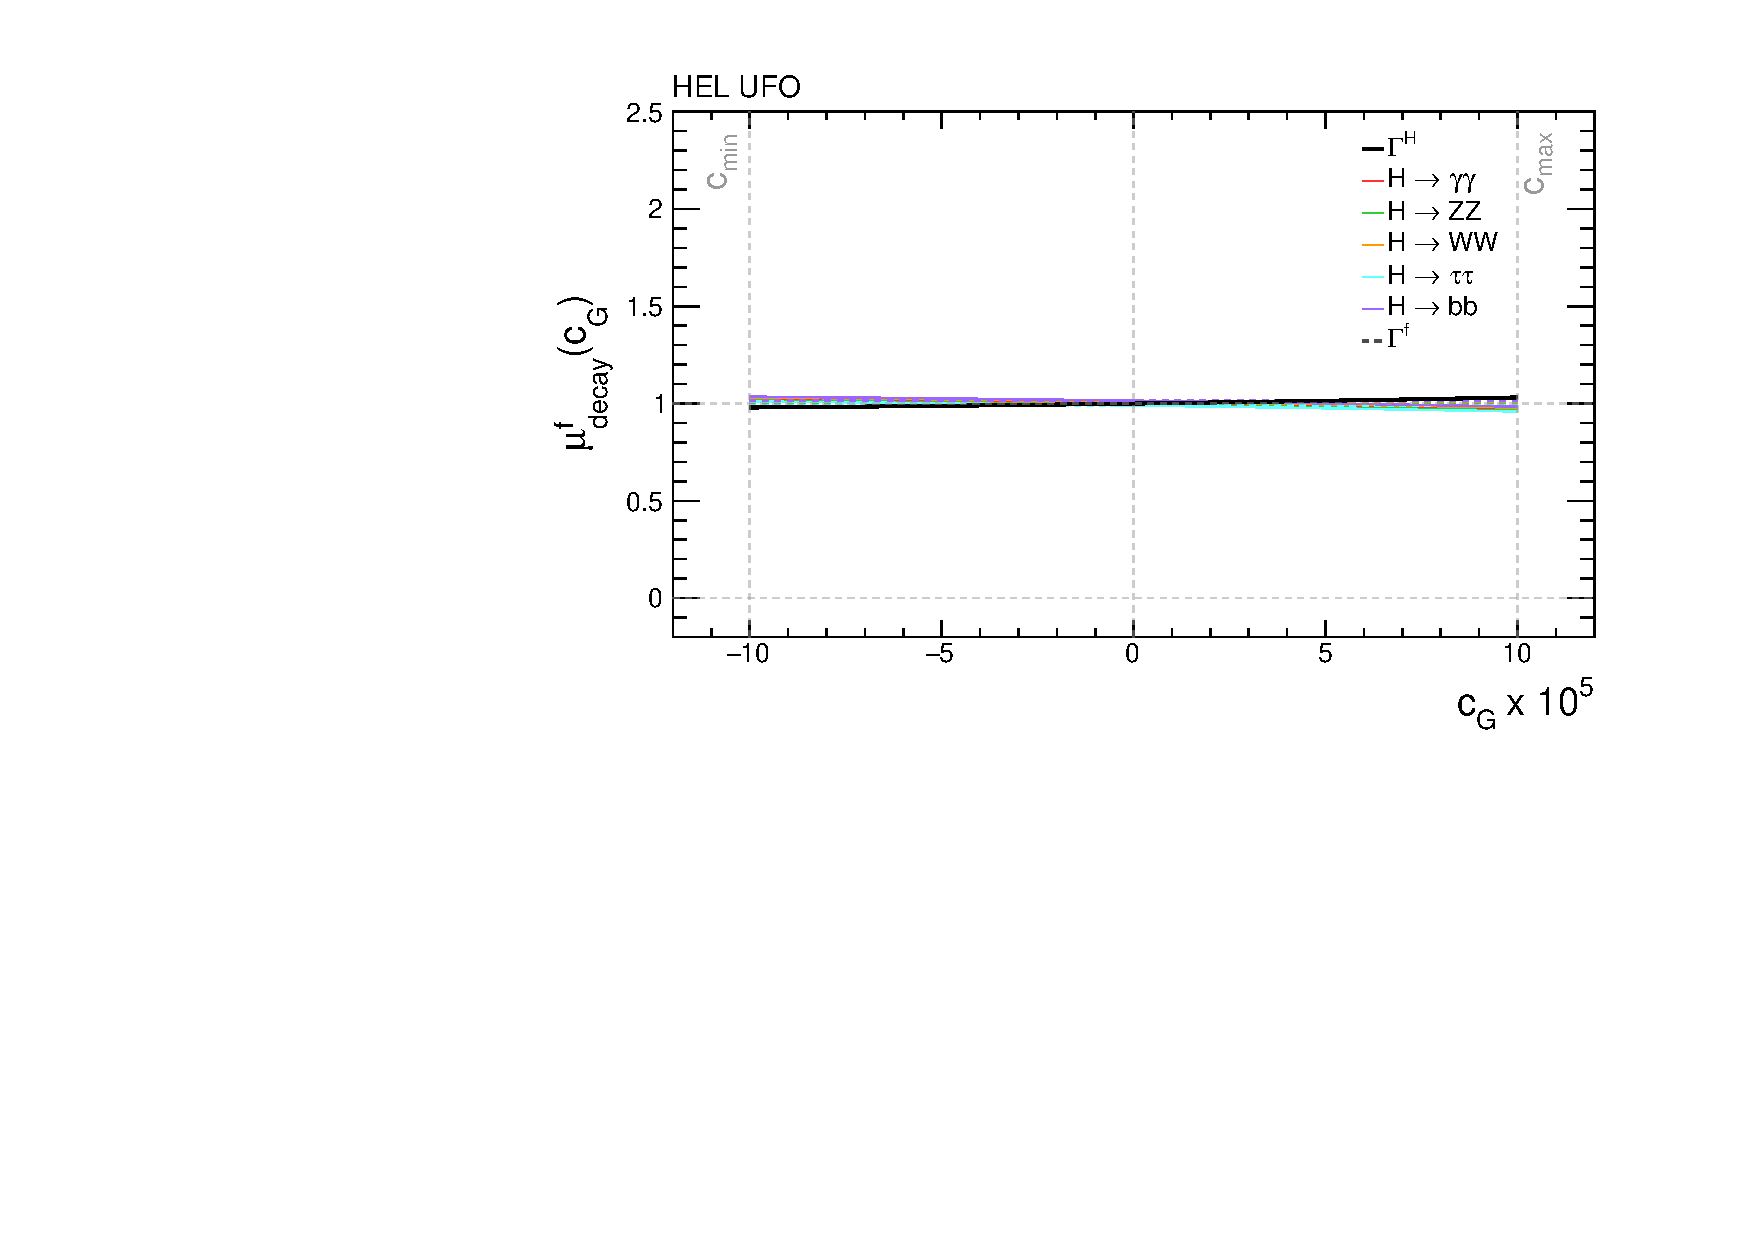
\includegraphics[width=.49\textwidth]{Figures/eft/scaling_functions/decay_vs_cG.pdf}
  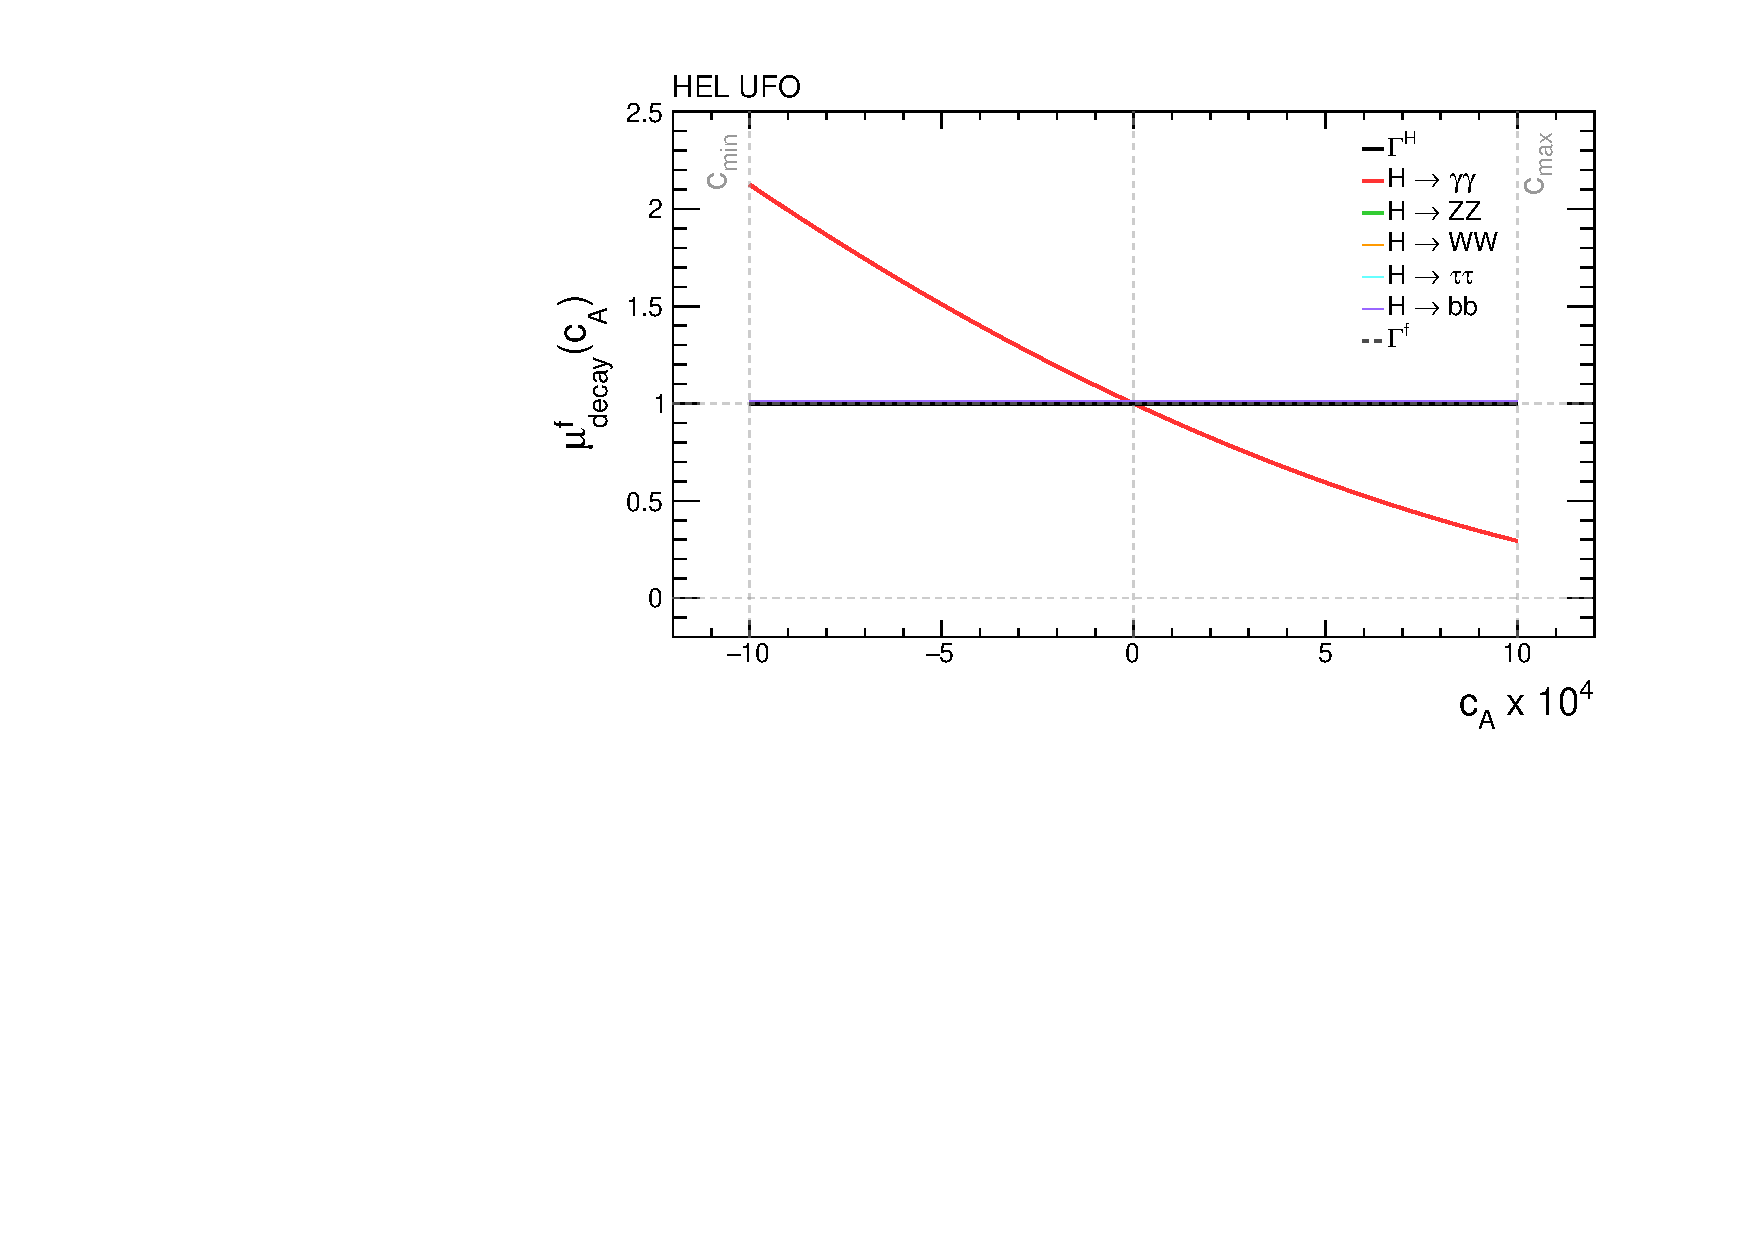
\includegraphics[width=.49\textwidth]{Figures/eft/scaling_functions/decay_vs_cA.pdf}
  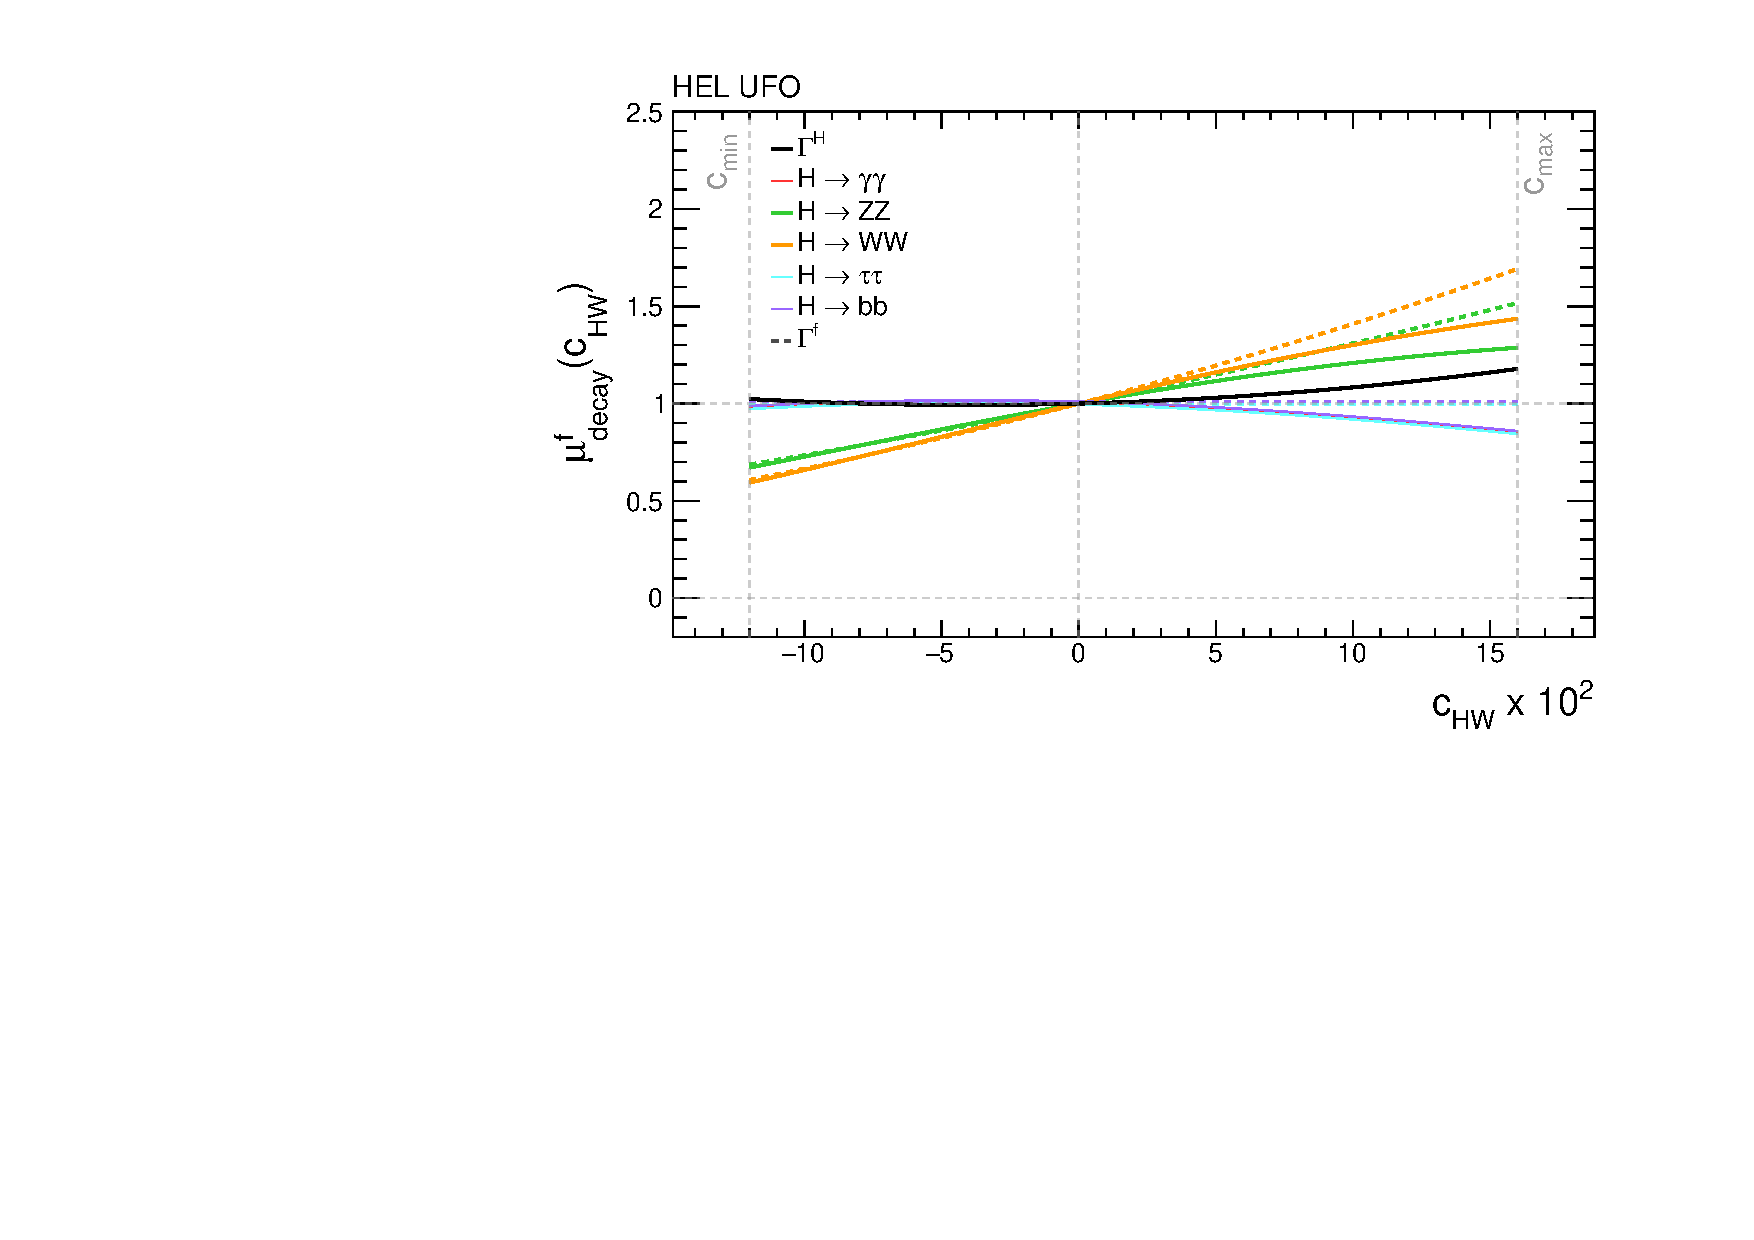
\includegraphics[width=.49\textwidth]{Figures/eft/scaling_functions/decay_vs_cHW.pdf}
  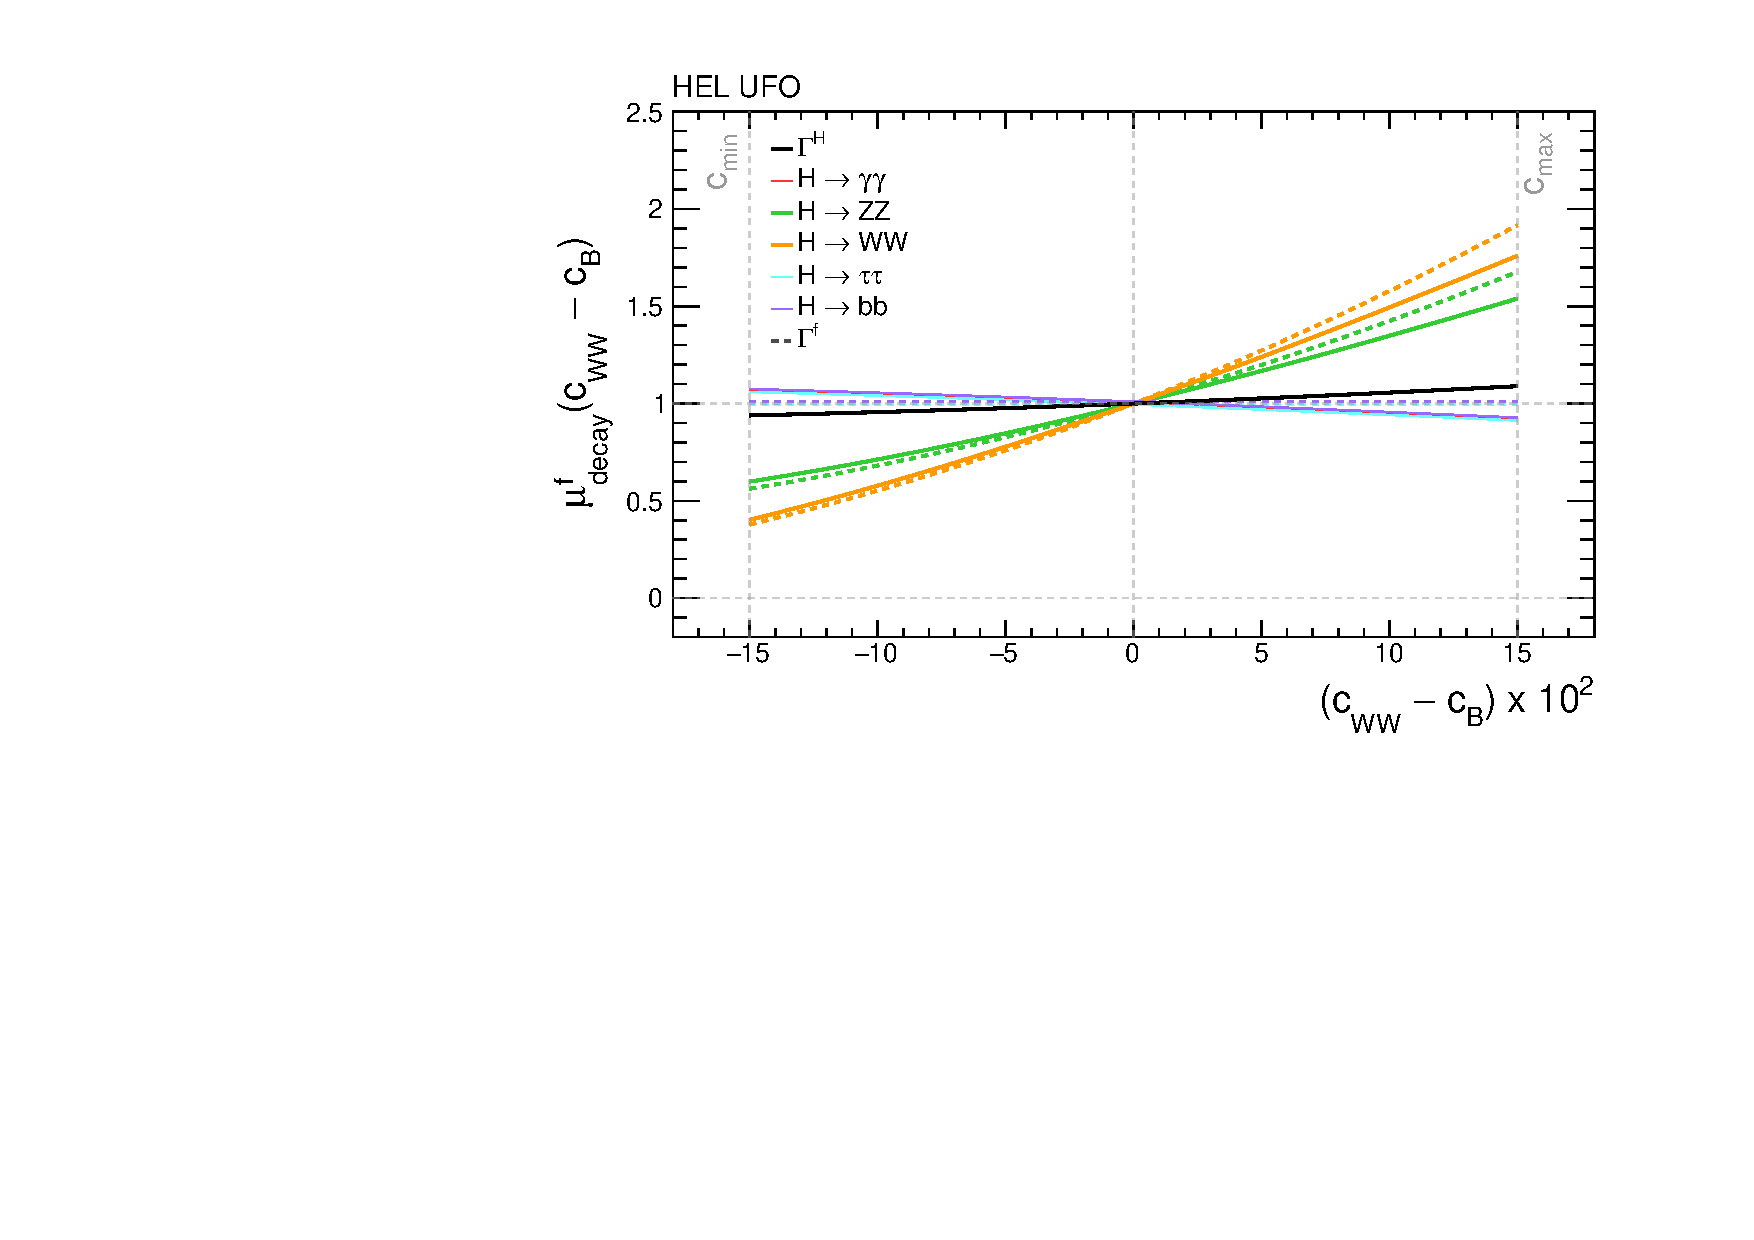
\includegraphics[width=.49\textwidth]{Figures/eft/scaling_functions/decay_vs_cWWMinuscB.pdf}
  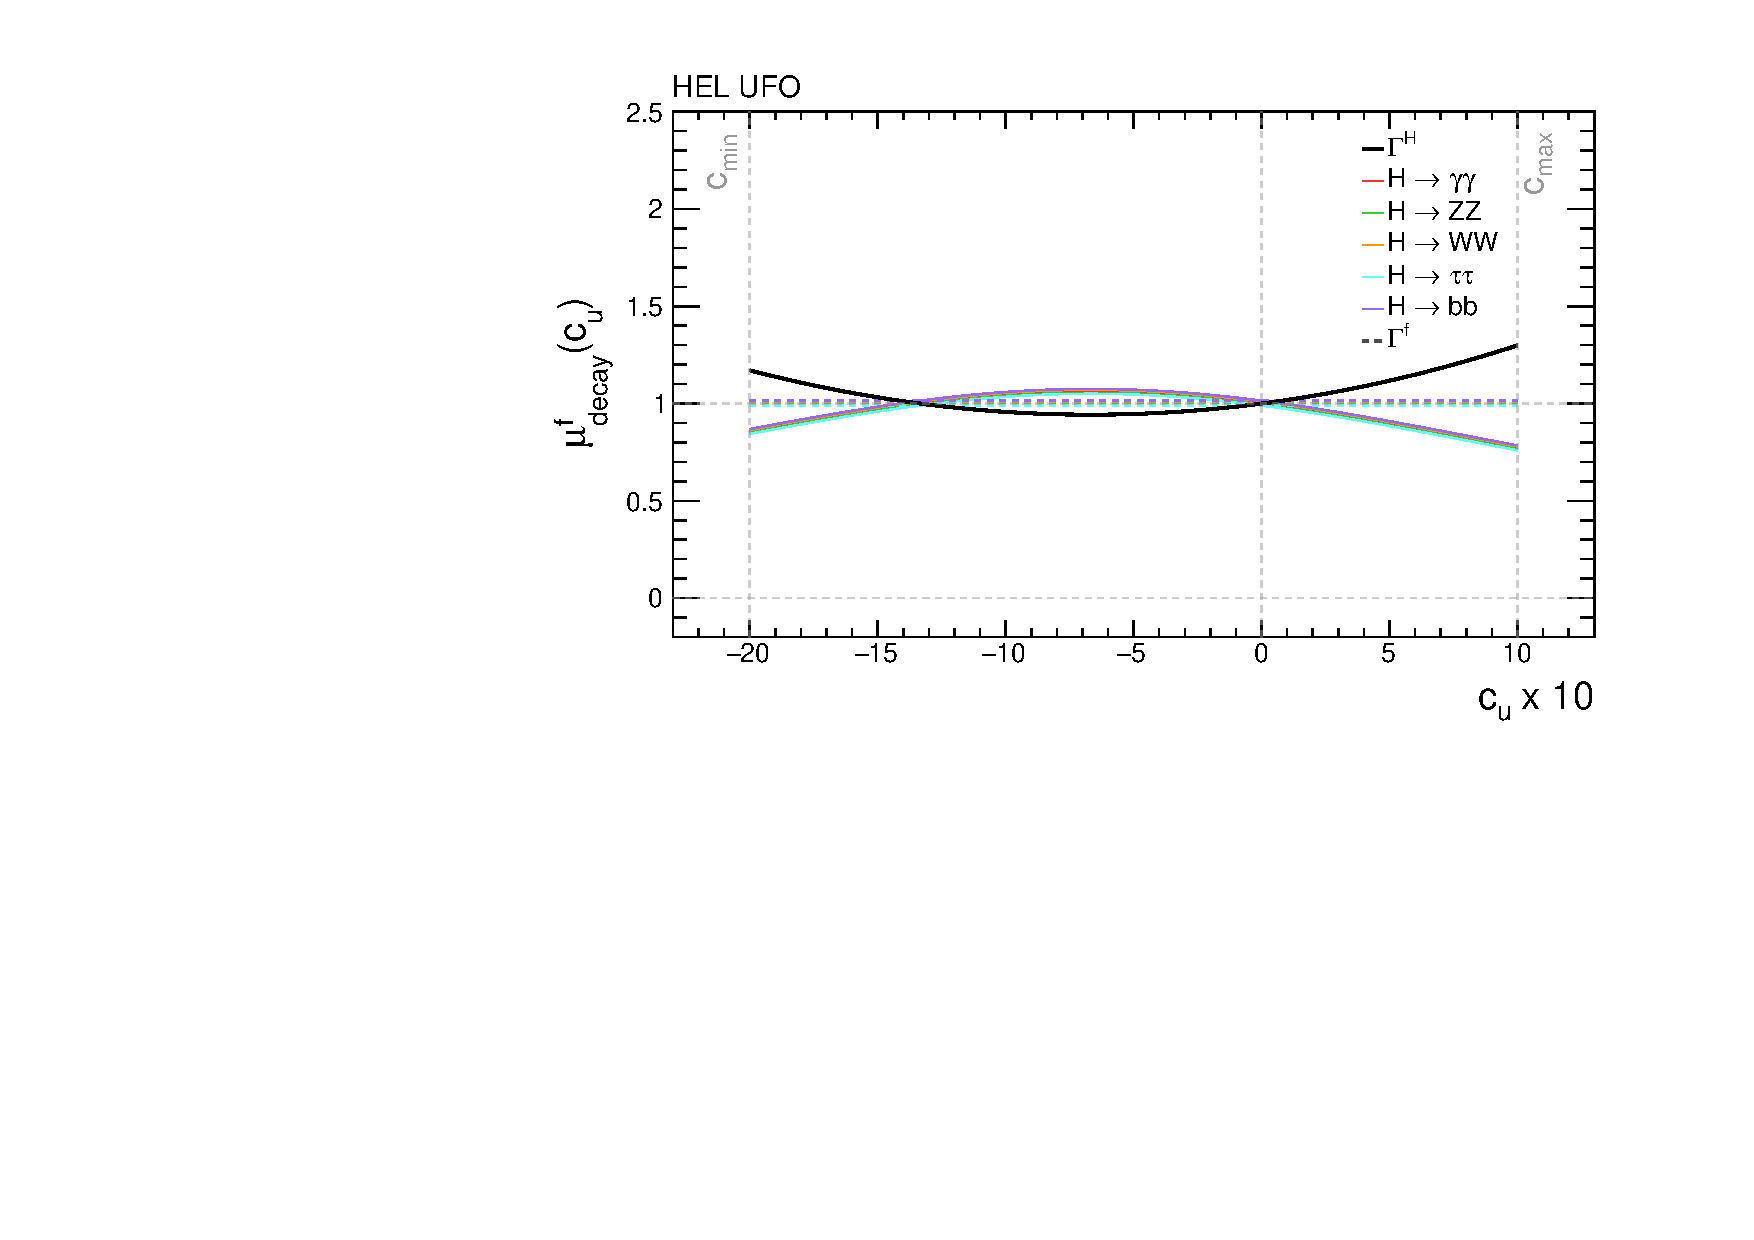
\includegraphics[width=.49\textwidth]{Figures/eft/scaling_functions/decay_vs_cu.pdf}
  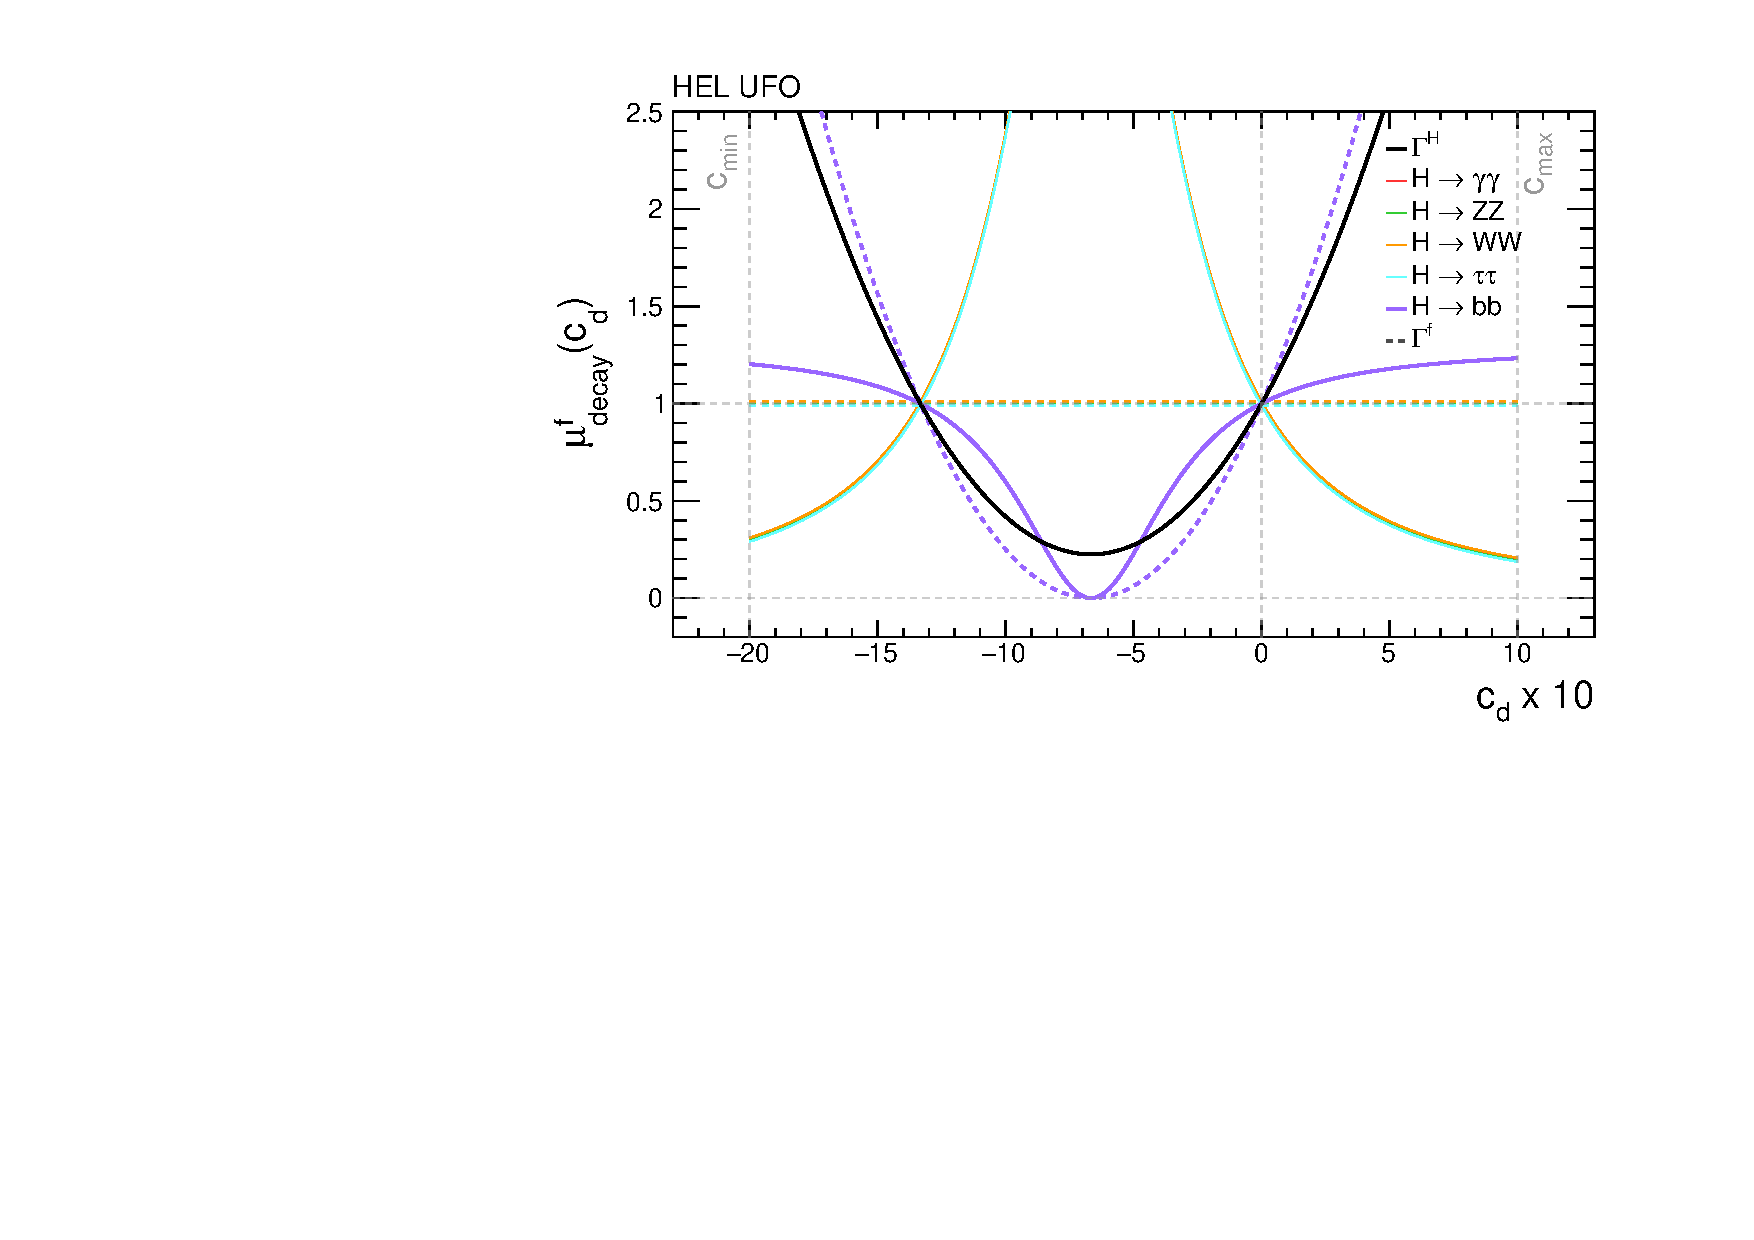
\includegraphics[width=.49\textwidth]{Figures/eft/scaling_functions/decay_vs_cd.pdf}
  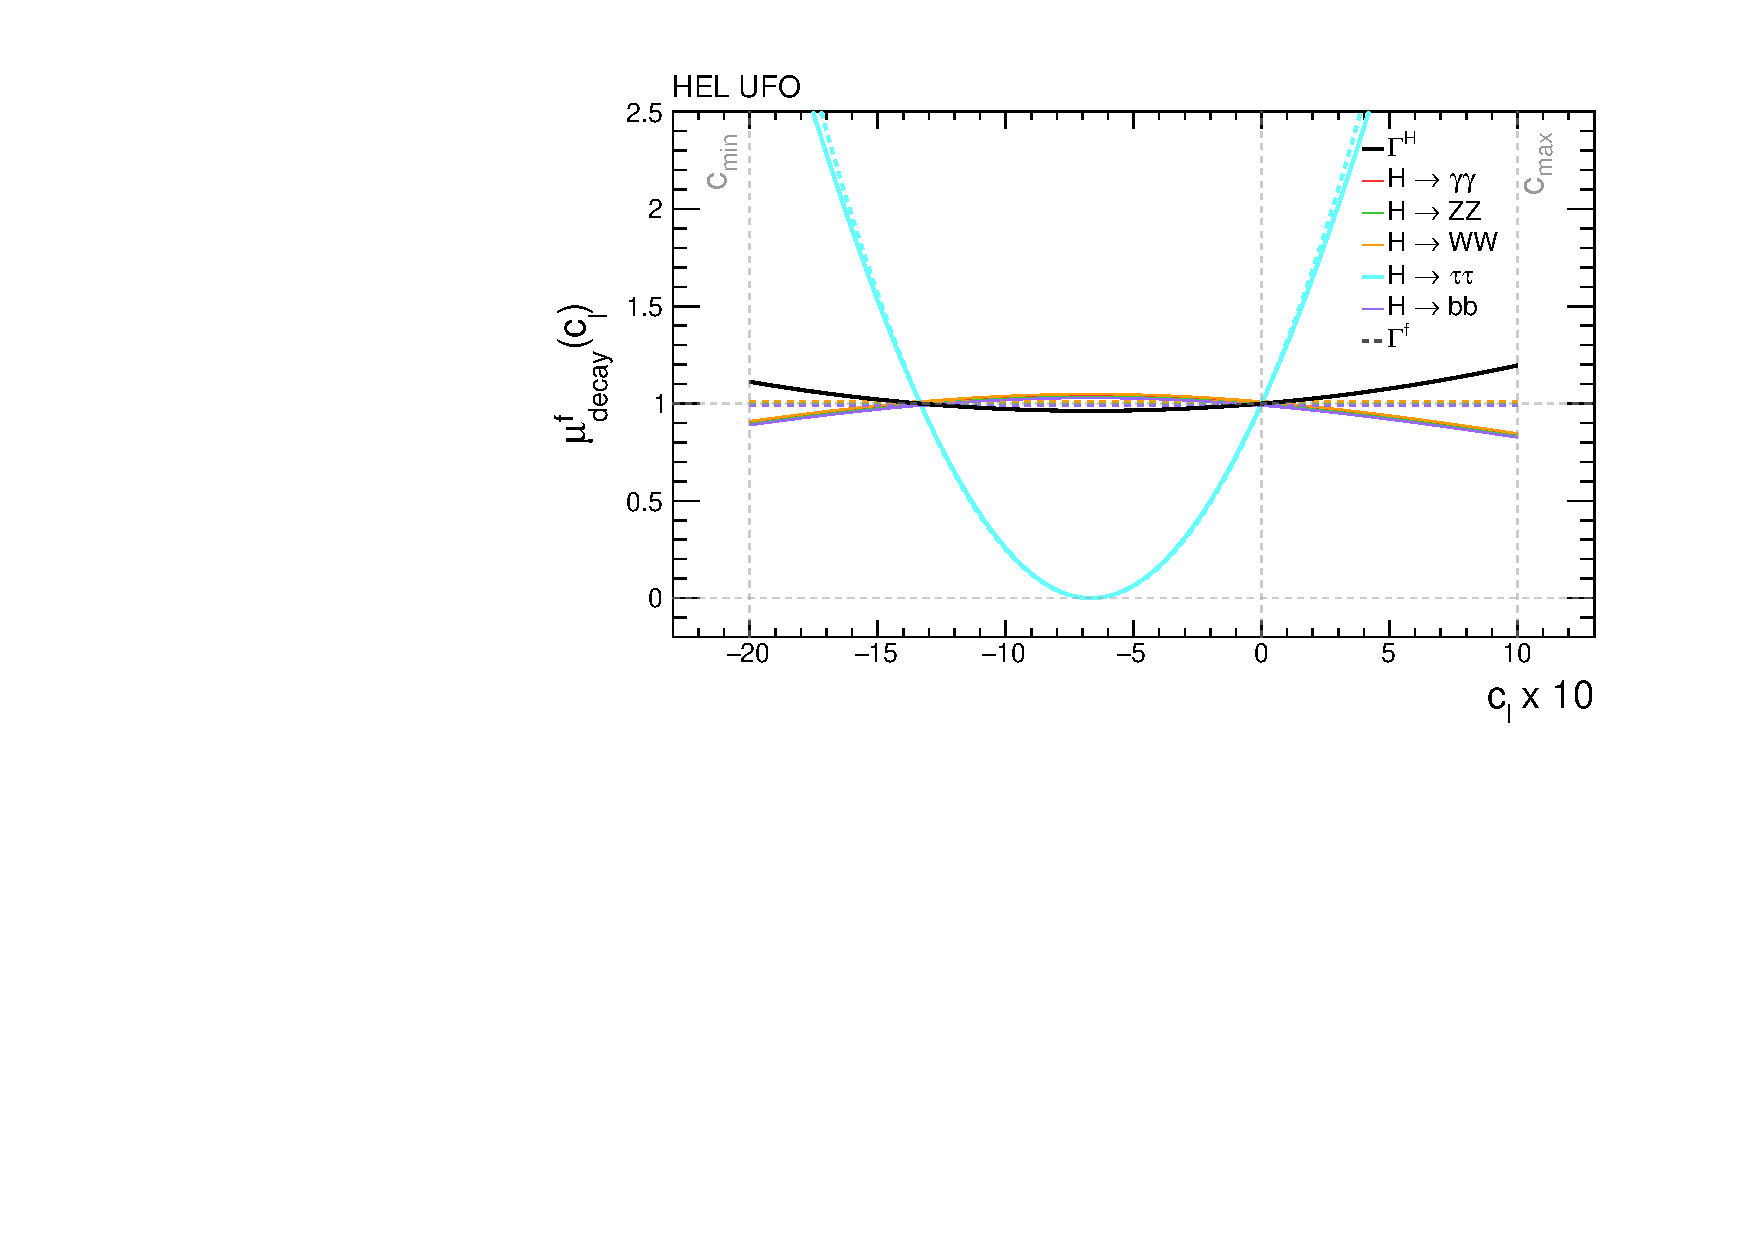
\includegraphics[width=.49\textwidth]{Figures/eft/scaling_functions/decay_vs_cl.pdf}
  \caption[HEL branching fraction scaling functions]
  {
    Branching fraction scaling functions, $\mu_{\rm{decay}}^f(\vec{c})$, for each decay channel considered in the CMS Higgs boson combination. Each function is decomposed into the partial width (dashed lines) and total width (solid black line) scalings.
  }
  \label{fig:eft_decay}
\end{figure}

\subsection{Summary}
The impacts of each HEL parameter on the stage 0, 1.0 and 1.1 cross sections, and the branching fractions are displayed in Figure \ref{fig:hel_summary}, relative to the SM predictions. Each parameter is varied to it's expected upper and lower $1\sigma$ confidence level values to indicate the size of variations to which the combination measurements are sensitive to\footnote{These are taken from the fit in which only variations in a single HEL parameter are considered (see section \ref{sec:eft_results})}. For parameters which demonstrate a double-minimum in the likelihood ($c_u$,$c_d$,$c_\ell$), the upper confidence level is taken from the minimum around 0. 

\begin{figure}[htb!]
  \centering
  \hspace*{-1.4cm}
  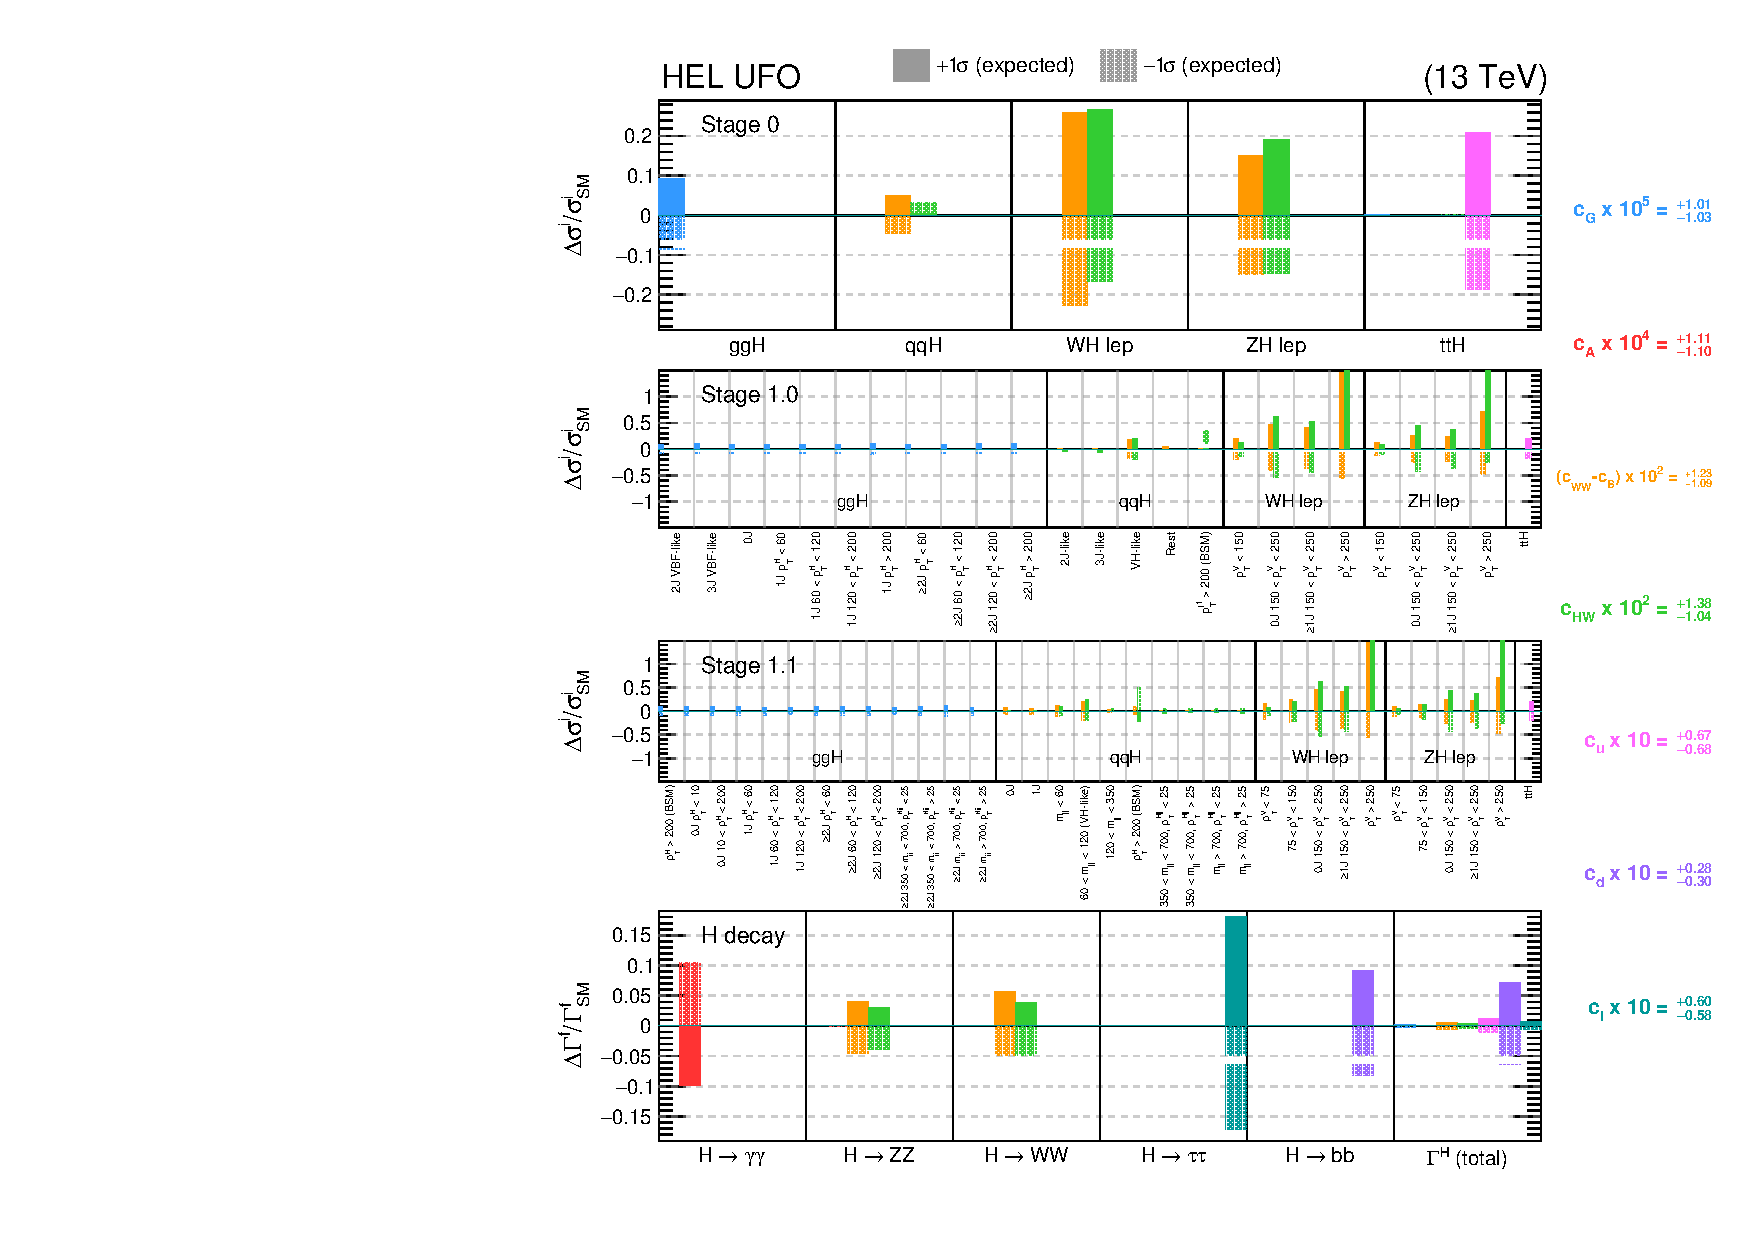
\includegraphics[width=1.2\textwidth]{Figures/eft/scaling_functions/HEL_summary.pdf}
  \hspace*{-1.4cm}
  \caption[HEL summary]
  {
    The impact of each HEL parameter on all STXS stage 0, stage 1.0 and stage 1.1 cross sections, and the relevant partial and total Higgs boson decay widths. Each parameter is varied to it's corresponding expected upper and lower $1\sigma$ confidence level values to indicate the size of variations to which the CMS Higgs boson combination is sensitive to.
  }
  \label{fig:hel_summary}
\end{figure}

The full HEL parametrisation, $\mu_{\rm{prod}}^i(\vec{c})$ and $\mu_{\rm{decay}}^f(\vec{c})$, is presented in Tables XX-YY of Appendix~\ref{app:hel_parametrisation}. For each signal process, the total scaling function is defined as the product of the corresponding cross section and branching fraction scaling functions. Figure \ref{fig:hel_total_example} shows the example for the qqH BSM STXS stage 1.1 bin in the \Hfl decay channel, plotted as a function of $(c_{WW}-c_B)$-vs-$c_{HW}$. These total scaling functions are then applied to the signal yield estimates when constructing the likelihood, as shown in equation \ref{eq:signal_yield_eft}, and constraints on the HEL parameters, $\vec{c}$, are extracted using the techniques described in section \ref{sec:results_extraction}.

\begin{figure}[htb!]
  \centering
  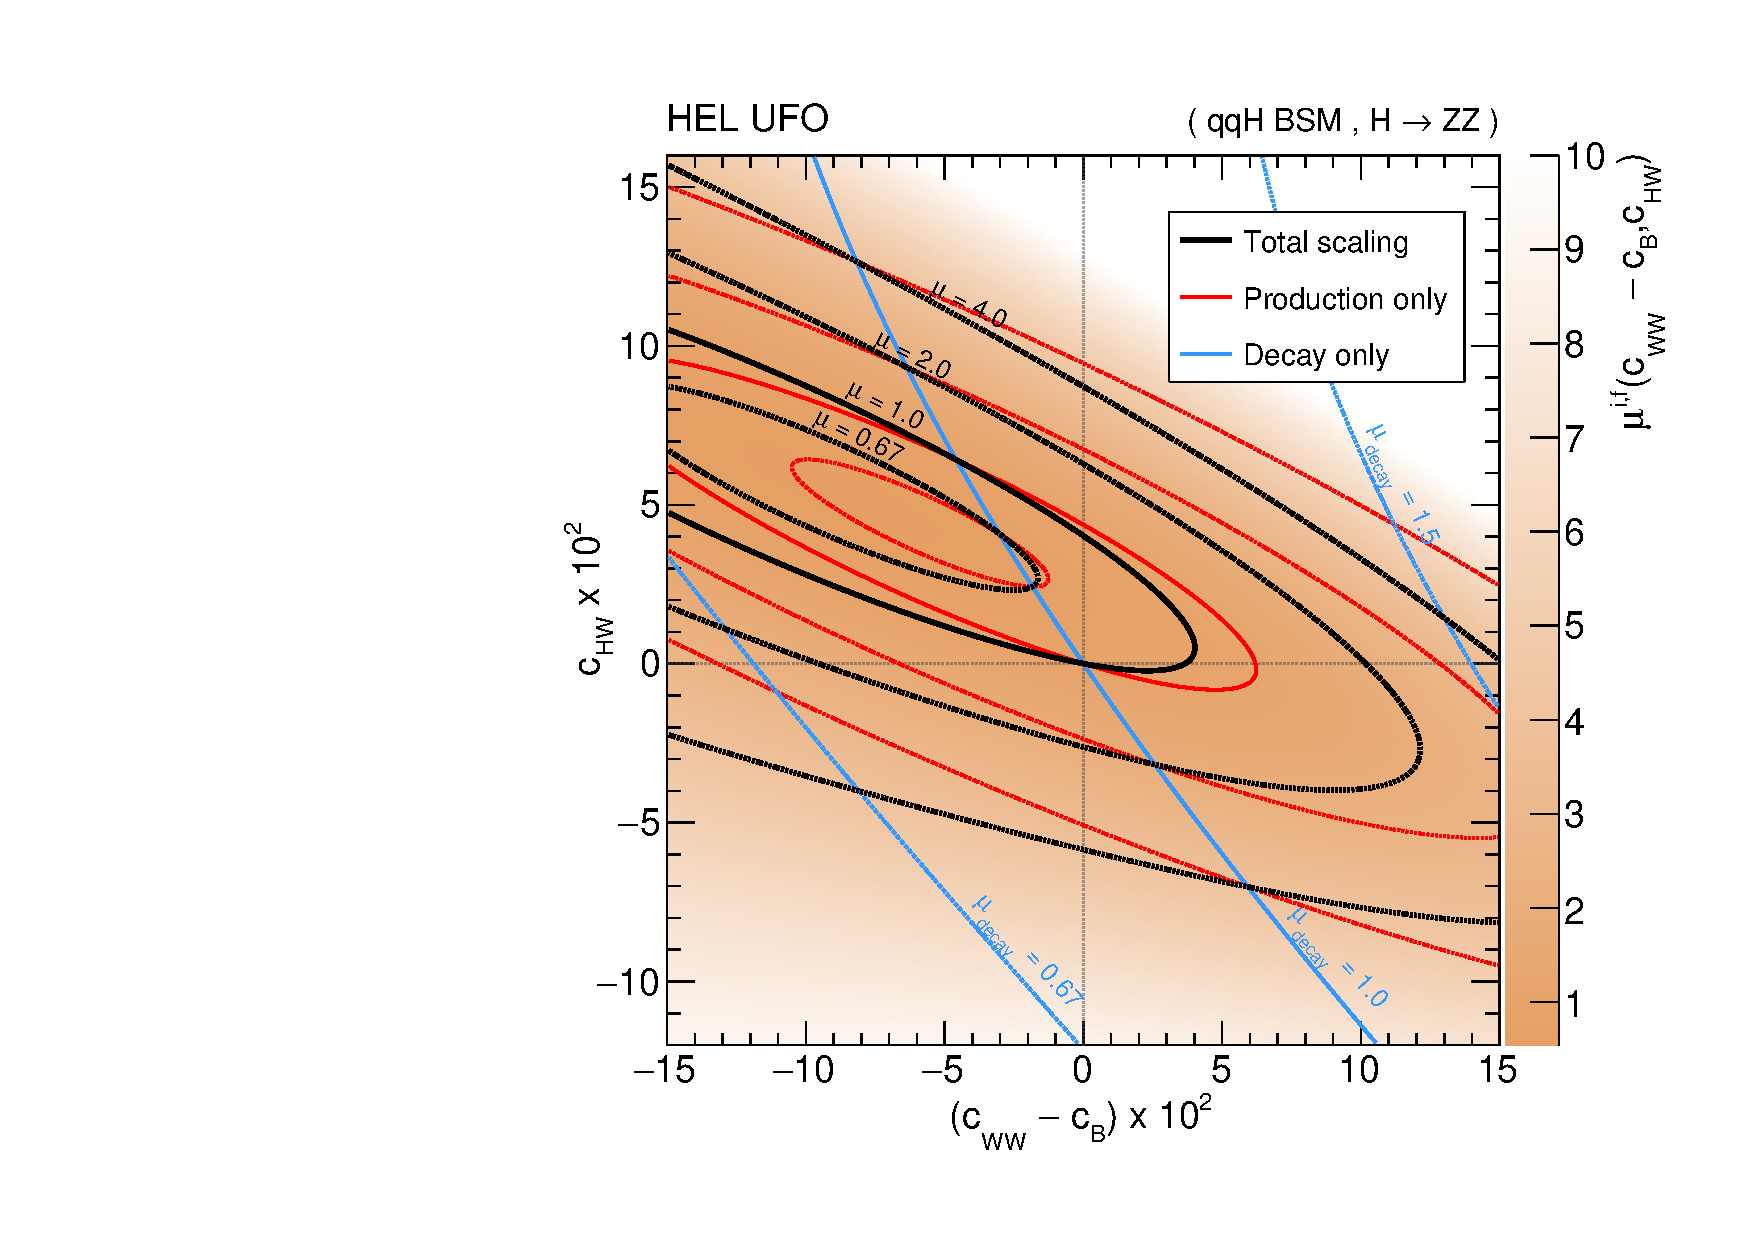
\includegraphics[width=.7\textwidth]{Figures/eft/scaling_functions/qqH_BSM_hzz_cWWMinuscB_vs_cHW.pdf}
  \caption[Two-dimensional HEL total scaling function example]
  {
    The total scaling function, $\mu^{i,f}(\vec{c})$, for qqH BSM events in the \Hfl decay channel, considering variations in the pair of HEL parameters: $(c_{WW}-c_B)$ and $c_{HW}$. The contours indicate lines of constant $\mu$. The effect is decomposed into the cross section scaling function, $\mu_{\rm{prod}}^i(\vec{c})$ (red), and branching fraction scaling function $\mu_{\rm{decay}}^f(\vec{c})$ (blue).
  }
  \label{fig:hel_total_example}
\end{figure}

\subsection{Validation of the scaling functions}\label{sec:hel_validation}
The cross section scaling functions have been calculated previously for the STXS stage 1.0 bin definitions in Ref.~\cite{Hays:2673969}. This enables a direct comparison of the prefactors, $A_p$ and $B_{pr}$, calculated there (HXSWG parametrisation) to those used in this thesis (CMS parametrisation). For most stage 1.0 bins the two parametrisations are in excellent agreement, with the calculated prefactors exhibiting differences below the 10\% level. This is not the case for the linear terms for a number of bins in the qqH binning scheme, particularly the qqH bin with $p_T$ of the leading jet greater than 200~GeV, the qqH VH-like bin, and the qqH rest bin. For such bins, the $A_{HW}$ and $A_{WW-B}$ values were found to differ by at least 50\%, with some even showing opposite signs.

An extensive series of test were performed to try and reconcile these differences. These include changing the nominal point in parameter space in the event generation away from the SM, altering the \textsc{MG5\_aMC@NLO} and \textsc{Pythia8} options, and generating separate samples for each point in parameter space as opposed to using the reweighting procedure described in section~\ref{sec:hel_derivation}. In all cases, the calculated prefactors were consistent within statistical fluctuations, demonstrating the CMS parametrisation is stable to variations in the extraction method. 

Nevertheless, the effects of the parametrisation differences have been investigated. This was done by using the HXSWG parametrisation for the STXS stage 1.0 bins when performing the results extraction. It was found that the constraints on $(c_{WW}-c_B)$ and $c_{HW}$ improve by roughly 20\% and 25\% respectively, compared to results when using the CMS parametrisation. The constraints on all other HEL parameters were in excellent agreement.

\section{Simplified likelihood re-interpretation procedure}\label{sec:eft_simplified}
This section serves as an aside to the rest of this chapter and can be skipped without loss of understanding. Nevertheless, before showing the results extracted using the full likelihood, it is useful to introduce a simplified approach to \textit{re-interpreting} cross section measurements. This has been used as a tool to investigate particular properties of the HEL interpretation, such as the most important operators for the combination input analyses, and to gain an estimate of their respective sensitivity. A $\chi^2$ function is constructed using measurements from different input analyses,

\begin{equation}
    \chi^2(\vec{c}) = \sum_a (\mathbf{X}_a-\pmb{\mu})^T \mathbf{V}_a^{-1} (\mathbf{X}_a-\pmb{\mu}),
\end{equation}

\noindent
with the following inputs:

\begin{itemize}
    \item $a$: index to label the input analysis.
    \item $\mathbf{X}_a$: a vector of cross section times branching fraction measurements from analysis, $a$. The elements of the vector are the best-fit values of $[\sigma^i\cdot\mathcal{B}^f]_{\rm{obs}}$, relative to the SM prediction: $x^{i,f}_a=[\sigma^i\cdot\mathcal{B}^f]_{\rm{obs}}/[\sigma^i\cdot\mathcal{B}^f]_{\rm{SM}}$. For example, to use the \Hgg minimal merging results shown in chapter \ref{chap:hgg_results}, $\mathbf{X}_a$ would be a vector of the best-fit values shown in the final column of Table~\ref{tab:stage1p2_minimal_results}.
    \item $\pmb{\mu}$: a vector of EFT scaling functions, $\mu^{i,f}(\vec{c})$, where the elements match the corresponding measurement in the $\mathbf{X}_a$ vector: $x^{i,f}_a$. In this manner, the element-wise subtraction is minimised for the HEL parameter point in which $\mu^{i,f}(\vec{c})=[\sigma^i\cdot\mathcal{B}^f]_{\rm{obs}}/[\sigma^i\cdot\mathcal{B}^f]_{\rm{SM}}$.
    \item $\mathbf{V}_a$: covariance matrix for the cross section times branching fraction measurements from analysis, $a$, with elements: $V^{(i,f),(j,g)}_a = \rho_{(i,f),(j,g)}\Sigma_{i,f}\Sigma_{j,g}$. The terms $\Sigma_{i,f}$ and $\Sigma_{j,g}$ are the \textit{symmetrised} 68\% confidence intervals in the measurements $x^{i,f}_a$ and $x^{j,g}_a$, respectively. The term $\rho_{(i,f),(j,g)}$ refers to the correlation coefficient between $x^{i,f}_a$ and $x^{j,g}_a$. Note, if the input analysis corresponds to measurements in a single decay channel then $f=g$. To use the \Hgg minimal merging example, the $\Sigma_{i,f}$ and $\Sigma_{j,g}$ would be symmetrised values of the 68\% confidence intervals shown in the final column of Table~\ref{tab:stage1p2_minimal_results}, and $\rho_{(i,f),(j,g)}$ would be taken from the correlation matrix shown in Figure~\ref{fig:stage1p2_minimal_correlations}.
\end{itemize}

The $\chi^2$ value is minimised with respect to the HEL parameters, $\vec{c}$. This is done numerically using the \texttt{scipy.optimize} package~\cite{scipy}. The point in HEL parameter space which minimises $\chi^2$ corresponds to the best-fit point, whilst the points which incur a change, $\Delta\chi^2=1$~and~4, correspond to the $\pm1\sigma$ ($\sim$68\%) and $\pm2\sigma$ ($\sim$95\%) confidence intervals. This minimisation is performed for two scenarios. The first scenario, only considers variations in a single HEL parameter, whilst the other parameters are fixed to 0. The second scenario allows variations in all parameters simultaneously, performed by scanning over one parameter and profiling the other parameters in the minimisation. From a physical perspective, the first approach corresponds to considering BSM effects in a single EFT operator, whilst the second approach is more general and allows BSM effects in a number of operators simultaneously.

In summary, the $\Delta\chi^2(\vec{c})$ surface is a simplified approximation of the $q(\vec{c})$ surface, derived from the full combination likelihood. In this approximation, the likelihoods of the input analyses are assumed to be Gaussian in nature, such that the uncertainties in the measurements are symmetric. In addition, it is assumed that the results of different analyses are completely independent i.e. the correlation coefficients between them are 0. This assumption completely ignores the common sources of systematic uncertainty between input analyses.

\subsection{Re-interpreting CMS STXS measurements}\label{sec:hel_simplified_cms}
The simplified re-interpretation procedure is applied to the full set of input analyses listed in Table~\ref{tab:combination_inputs}. For both fitting scenarios, the $\chi^2$ minimisation is performed when using the full quadratic scaling functions, and when considering only the linear terms in the parametrisation ($B_{pr}=0$). A comparison between the two $\Delta\chi^2$ curves demonstrates the impact of including the purely-BSM terms, and therefore indicates the sensitivity of the measurement to terms suppressed by a factor $\Lambda^{-4}$. 

Figure \ref{fig:hel_chi2_simplified_0}--\ref{fig:hel_chi2_simplified_1} shows the $\Delta\chi^2(c_p)$ distributions as a function of each considered HEL parameter. The black and purple lines represent the fits in which the other parameters are profiled and fixed to zero, respectively. All results are in agreement with the SM ($c_p=0$) within the $2\sigma$ confidence intervals. In the plots, solid lines are used to show the results from using the full quadratic scaling functions, whilst the dashed lines represent the results from using the linear terms only. The inclusion of the quadratic terms is observed to have a particularly large impact on the $c_{HW}$ and $(c_{WW}-c_B)$ constraints. This effect can be inferred from the difference between the quadratic and linear scaling functions in Figure~\ref{fig:zhlep_sf_1d}, where for example, the ZH lep stage 0 bin (red line) has a steeper dependence for $c_{HW}>0$ when the quadratic terms are included. Consequently, the upper constraint on $c_{HW}$ in Figure~\ref{fig:hel_chi2_simplified_0} is tighter compared to the linear terms only case. In addition, the $c_u$, $c_d$ and $c_{\ell}$ $\Delta\chi^2$ curves exhibit a double minimum structure when the quadratic terms are included. All in all, these stark differences demonstrate the importance of including the $\Lambda^{-4}$-suppressed terms in the parametrisation\footnote{This finding questions the validity of neglecting dimension-8 operators, where the leading interference terms enter at $\mathcal{O}(\Lambda^{-4})$. This choice of only including dimension-6 operators effectively introduces some model-dependence into the interpretation. The definition of a fully-consistent SMEFT up to dimension-8 has recently been achieved~\cite{Murphy:2020rsh}.}.

The bottom panels of each plot show the pulls of the profiled HEL parameters as a function of the parameter of interest. These are taken from the fully quadratic fit (solid black line). The pulls can be used as an indication of the correlation between HEL parameters. For example, the $c_{HW}$ and $c_{WW}-c_B$ exhibit a strong anti-correlation due to their similar effects on the HWW and HZZ interaction vertices. The largest pulls are observed for the $c_d$ parameter. This is due to the sizeable impact on the total Higgs boson decay width from $c_d$, which in turn incurs a larger variation in the other profiled parameters.

In summary, the simplified re-interpretation procedure is a useful tool for extracting the approximate constraints on the parameters of interest, and testing the properties of the parametrisation, such as the impact of including the $B_{pr}$ terms. In addition, the pulls of the profiled parameters can be used to estimate their respective correlations. It should be stressed that this method is not particular to EFT. It can be used to re-interpret a wide range of LHC measurements in terms of some other BSM model, as long as the measurements, $\mathbf{X}_a$, can be expressed as functions, $\mu^{i,f}$, of the parameters of the underlying theory.

\begin{figure}[htb!]
  \centering
%   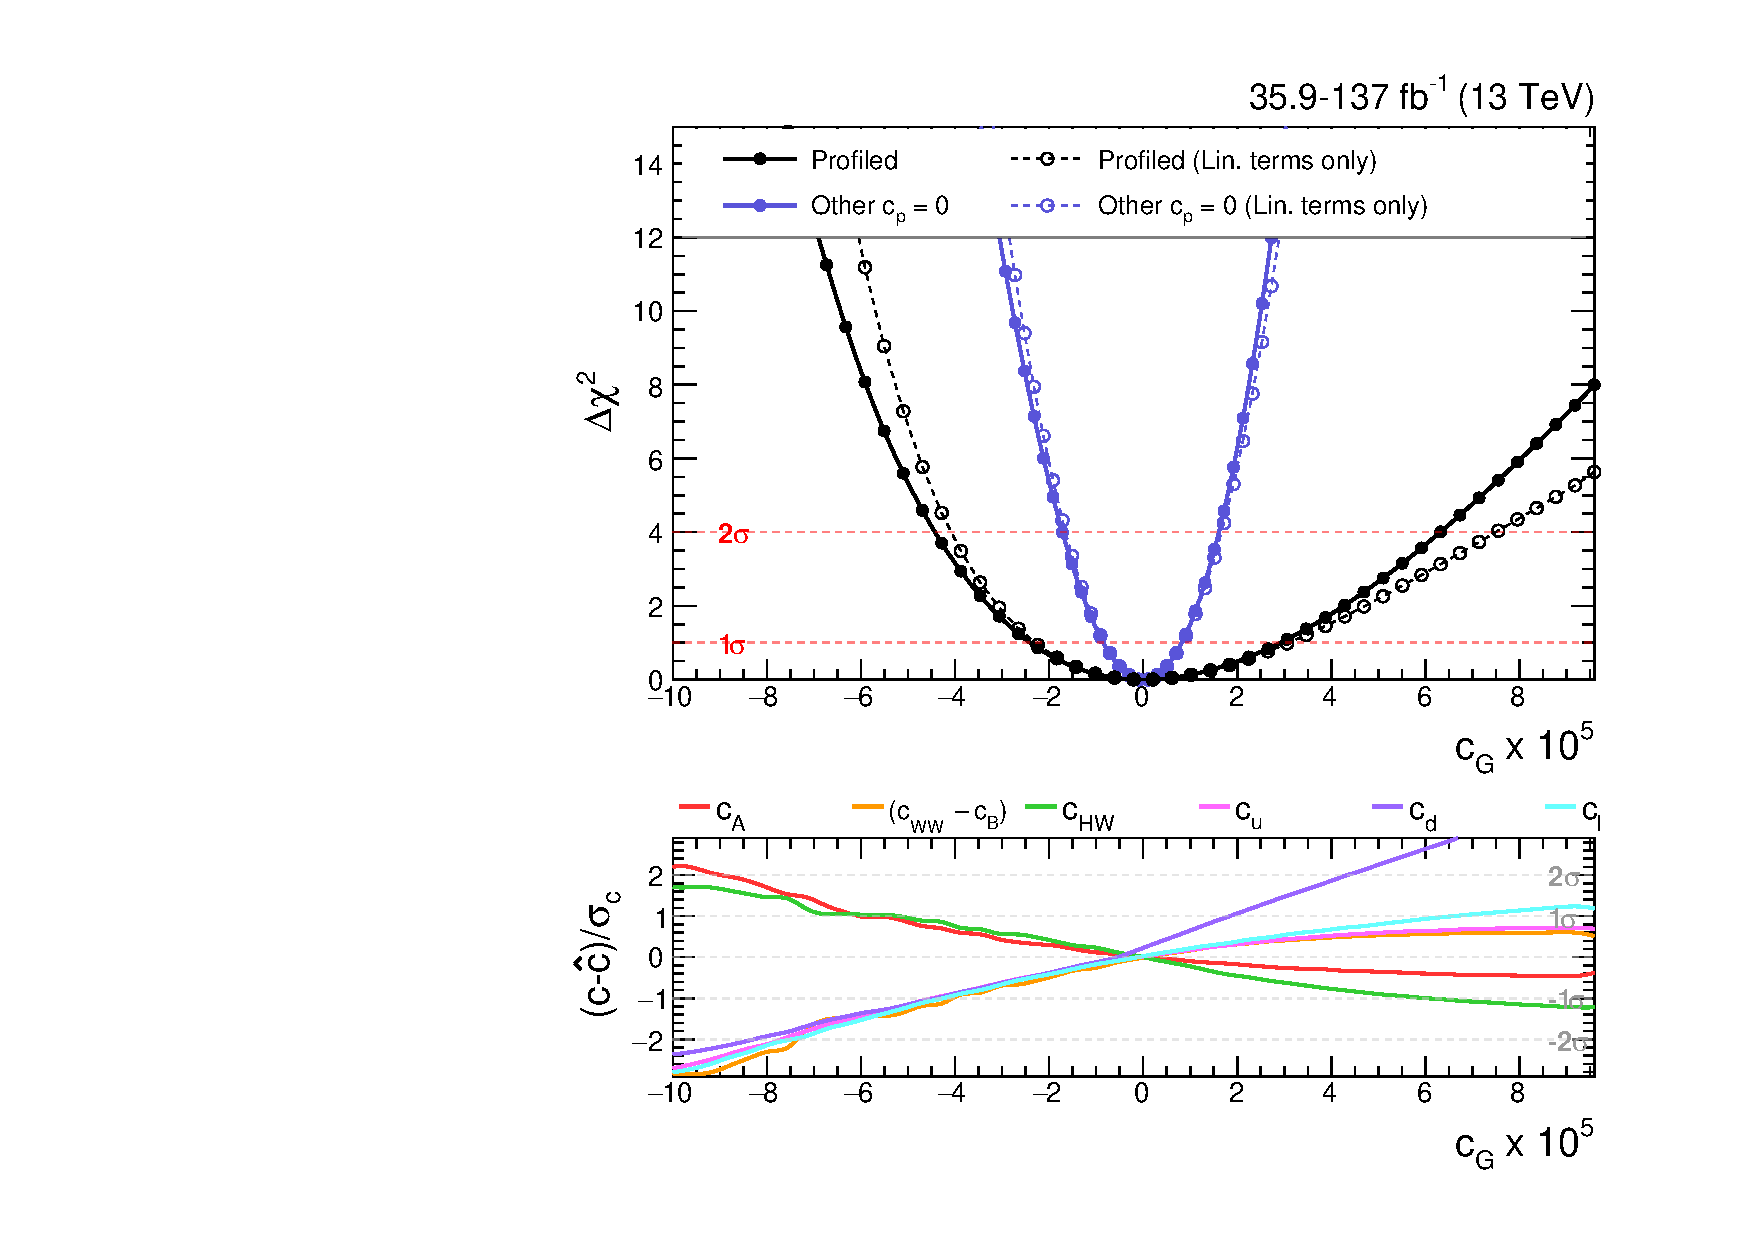
\includegraphics[width=.49\textwidth]{Figures/eft/chi2/expected/cG.pdf}
  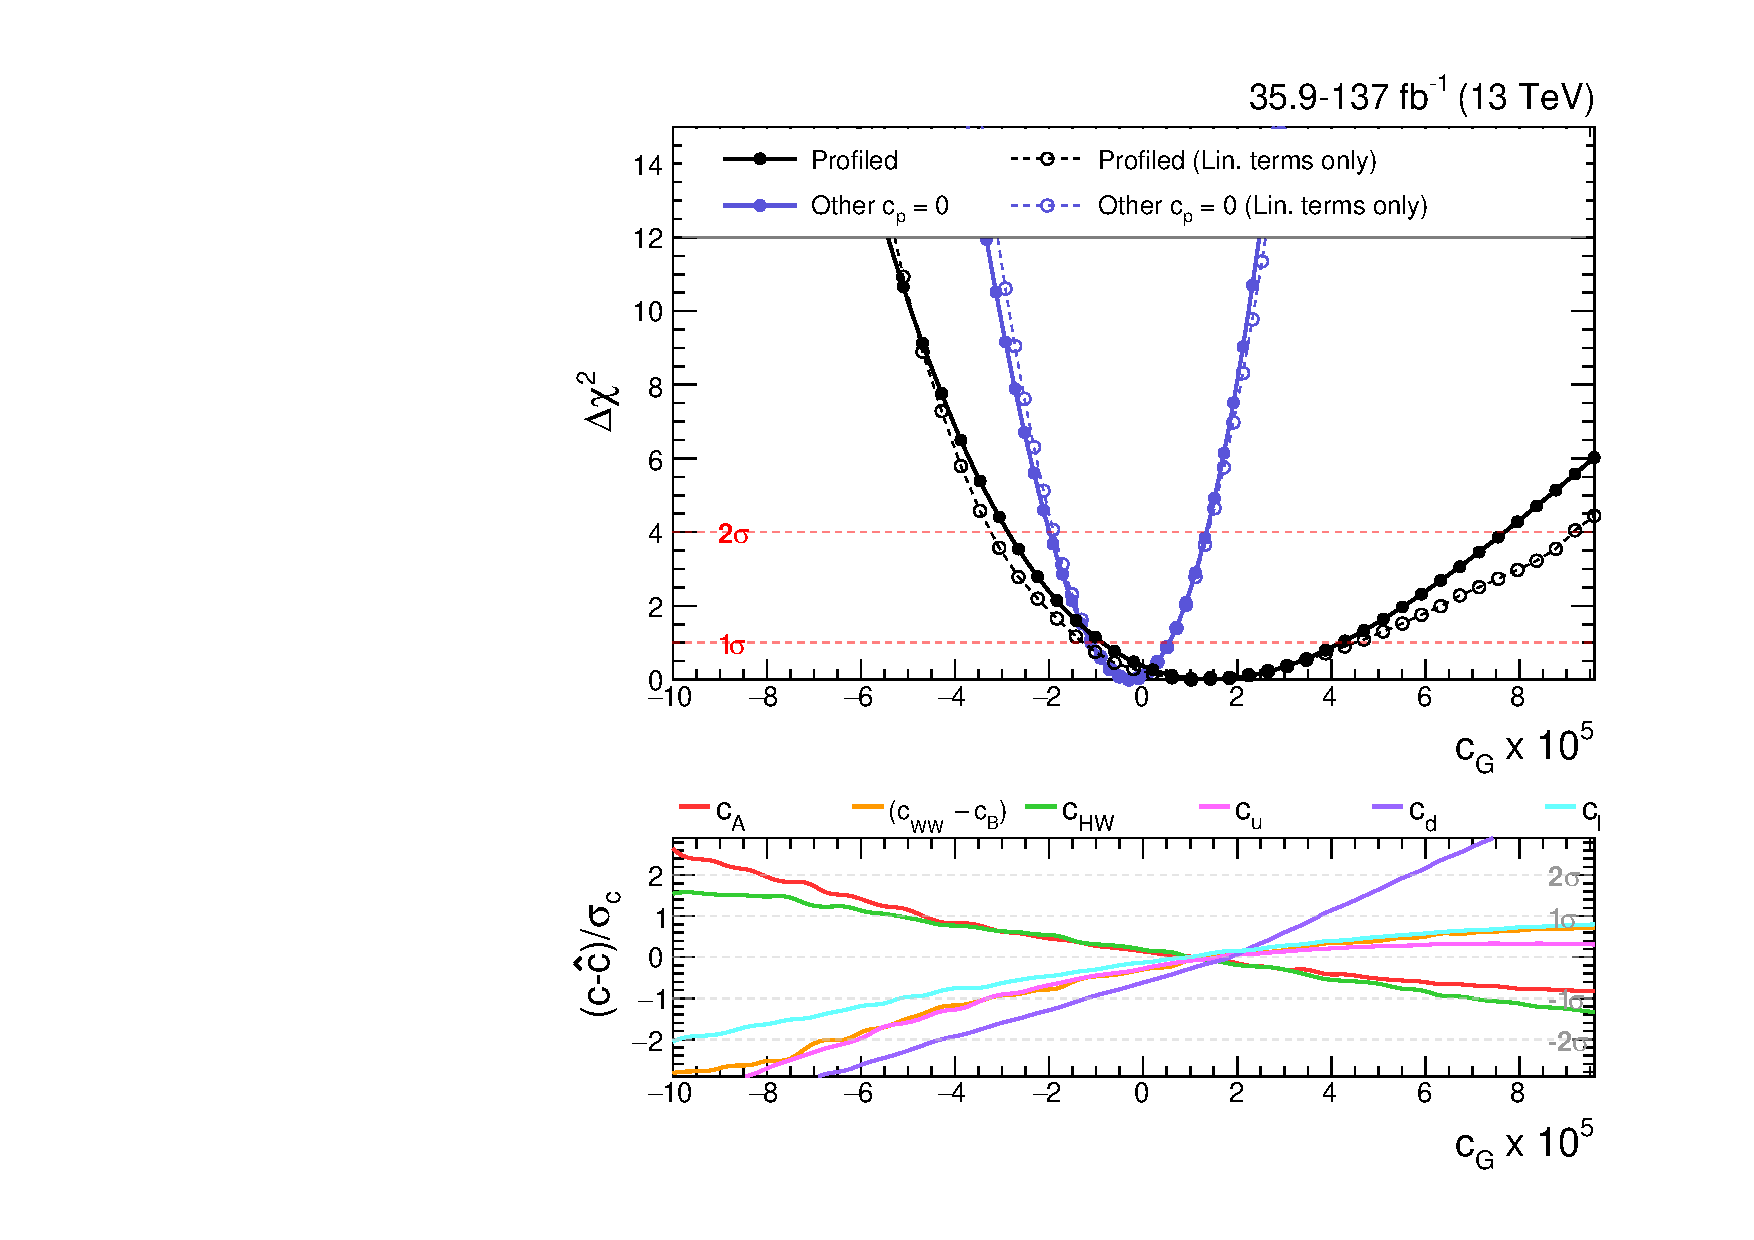
\includegraphics[width=.49\textwidth]{Figures/eft/chi2/observed/cG.pdf}
%   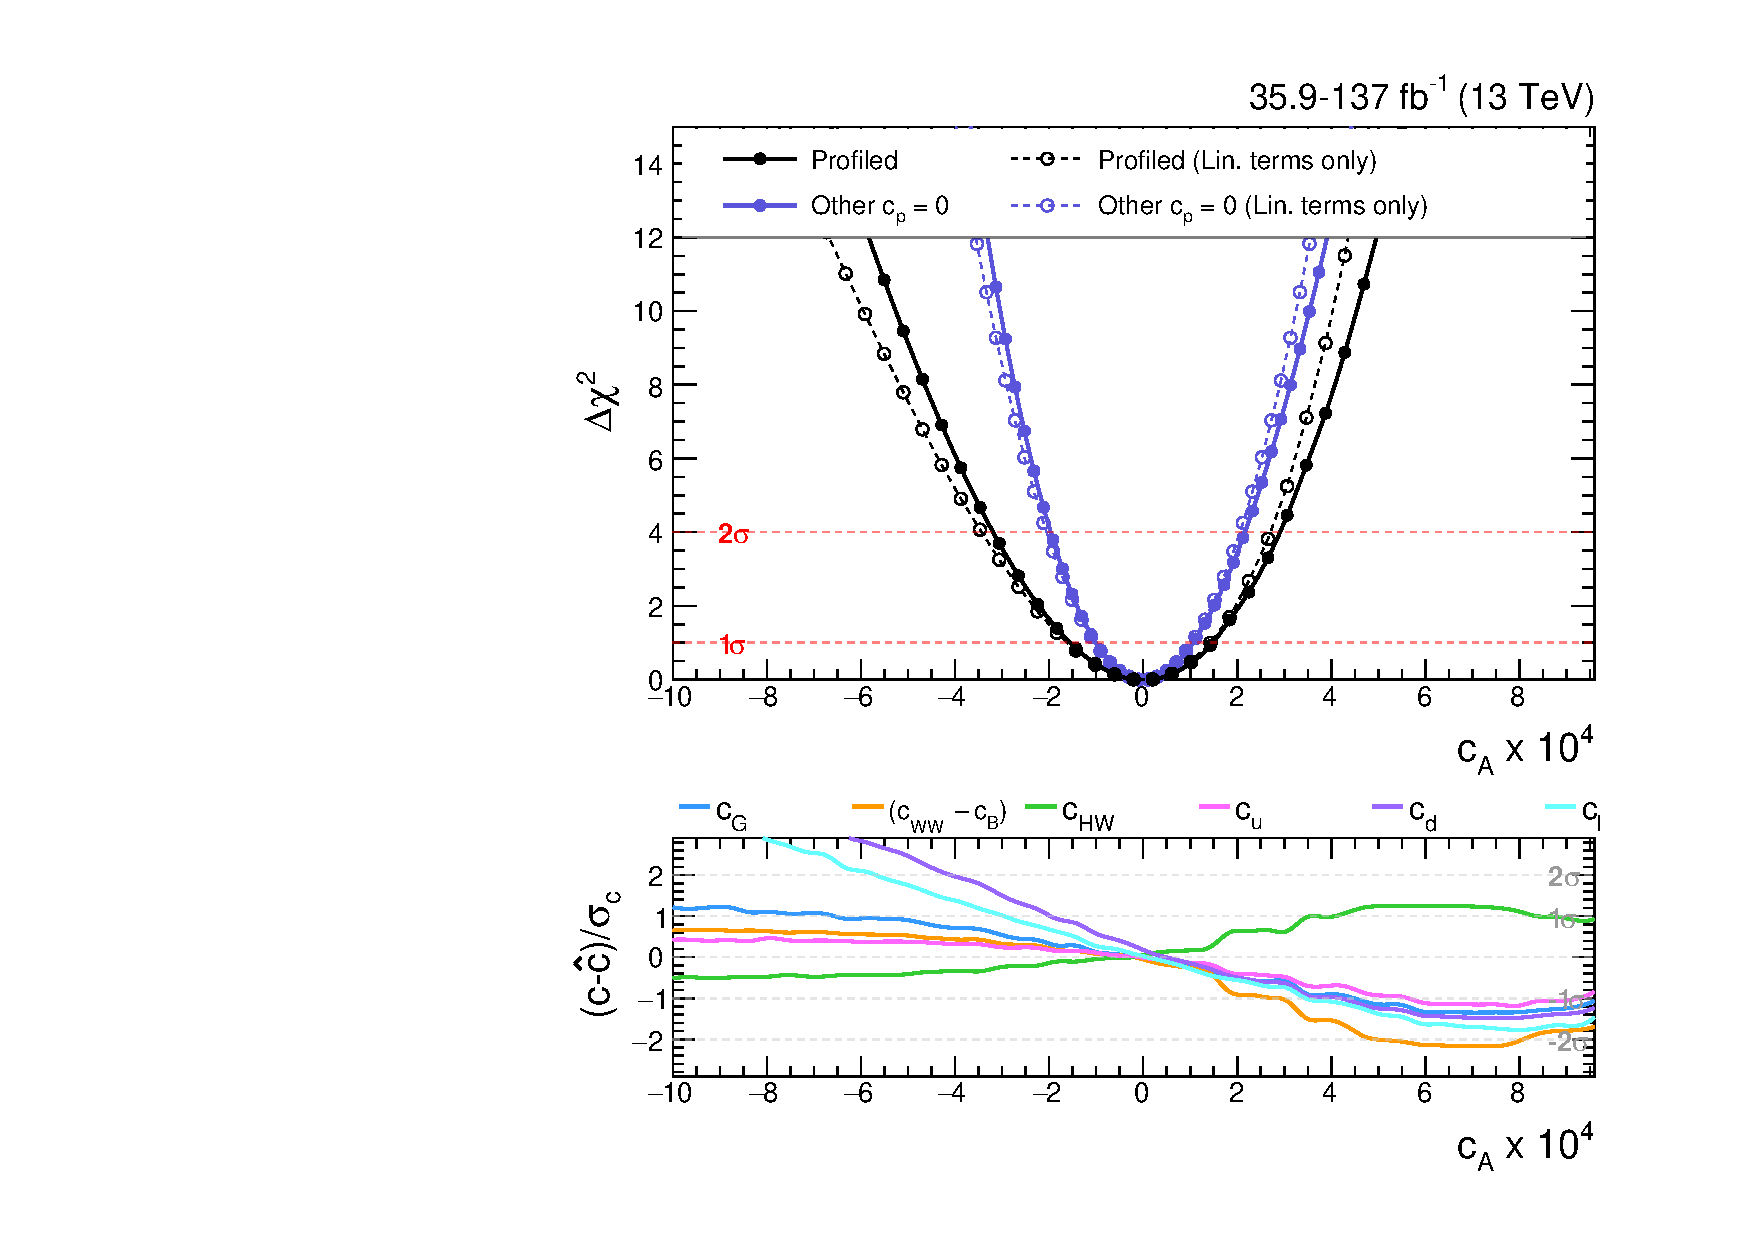
\includegraphics[width=.49\textwidth]{Figures/eft/chi2/expected/cA.pdf}
  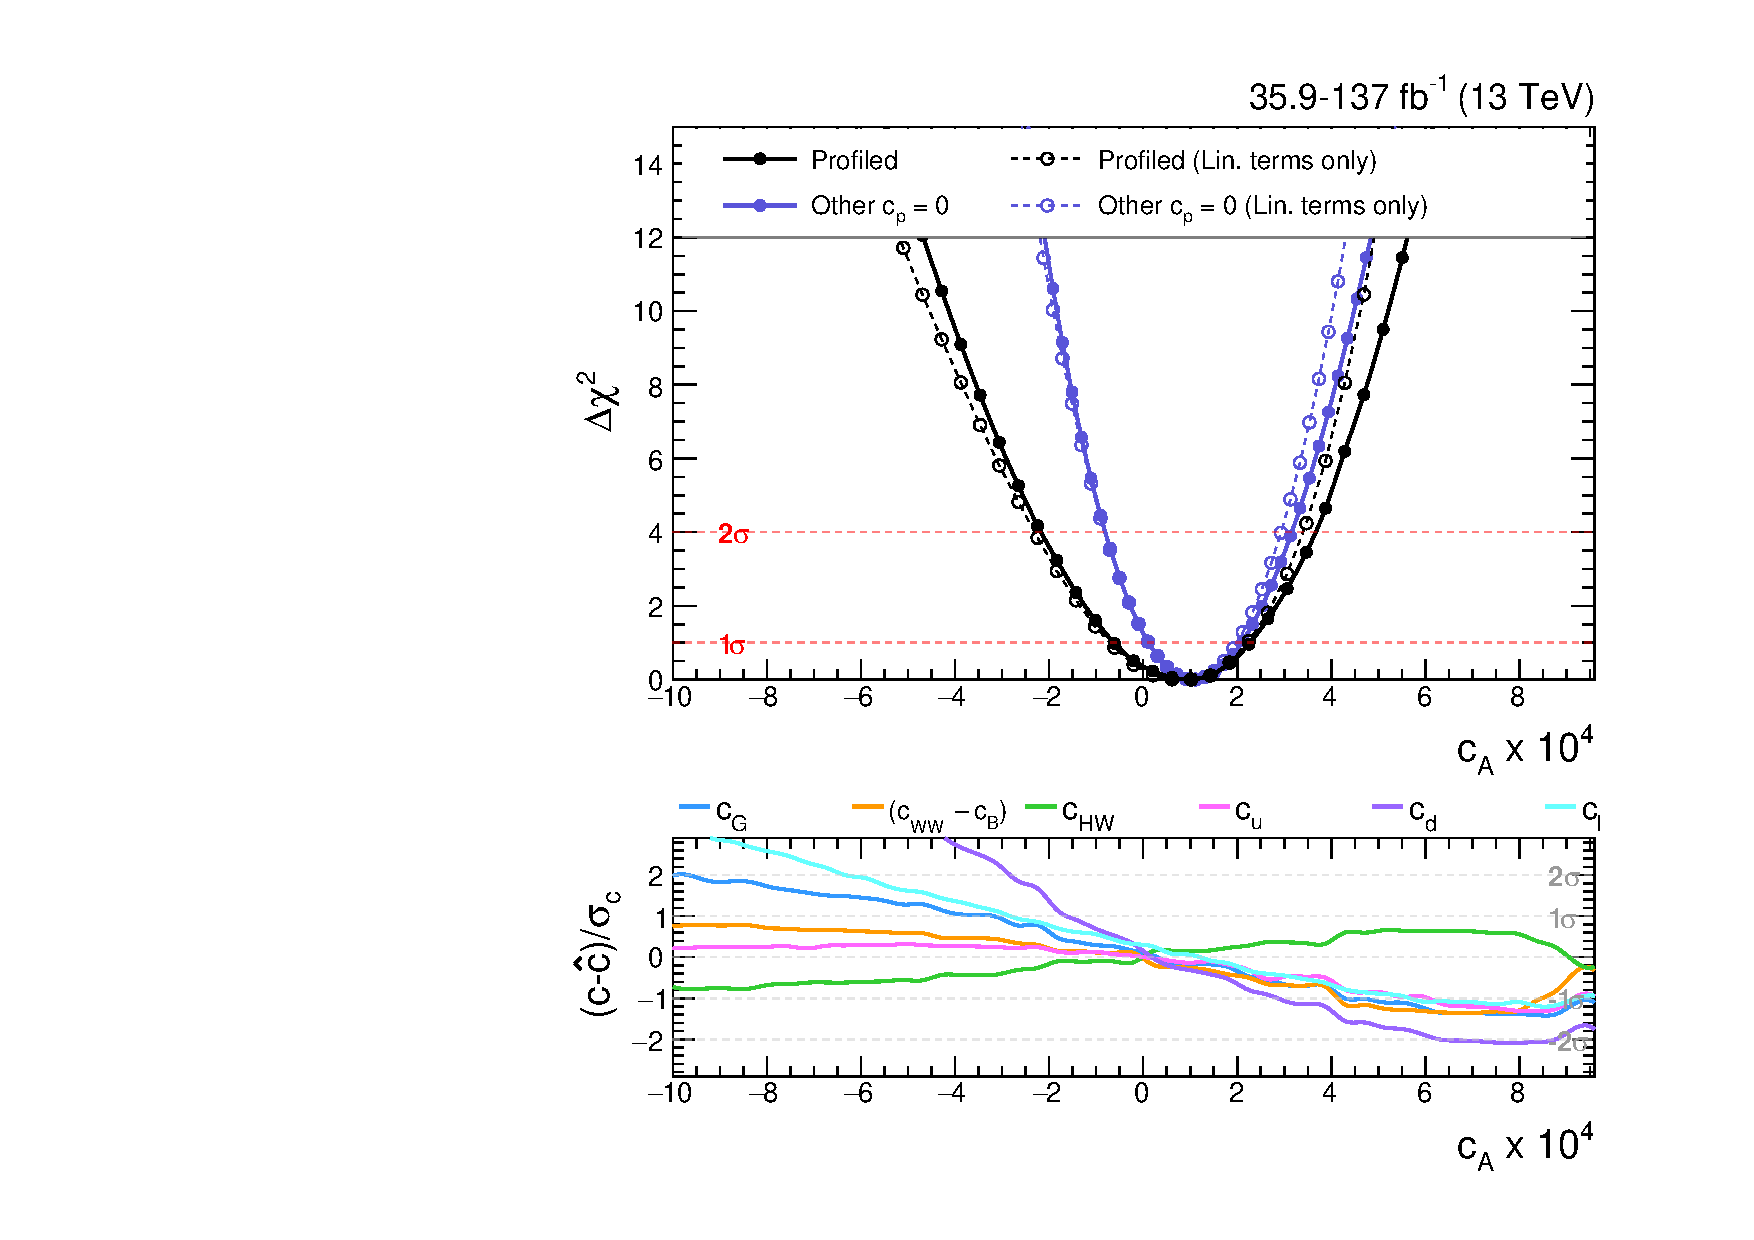
\includegraphics[width=.49\textwidth]{Figures/eft/chi2/observed/cA.pdf}
  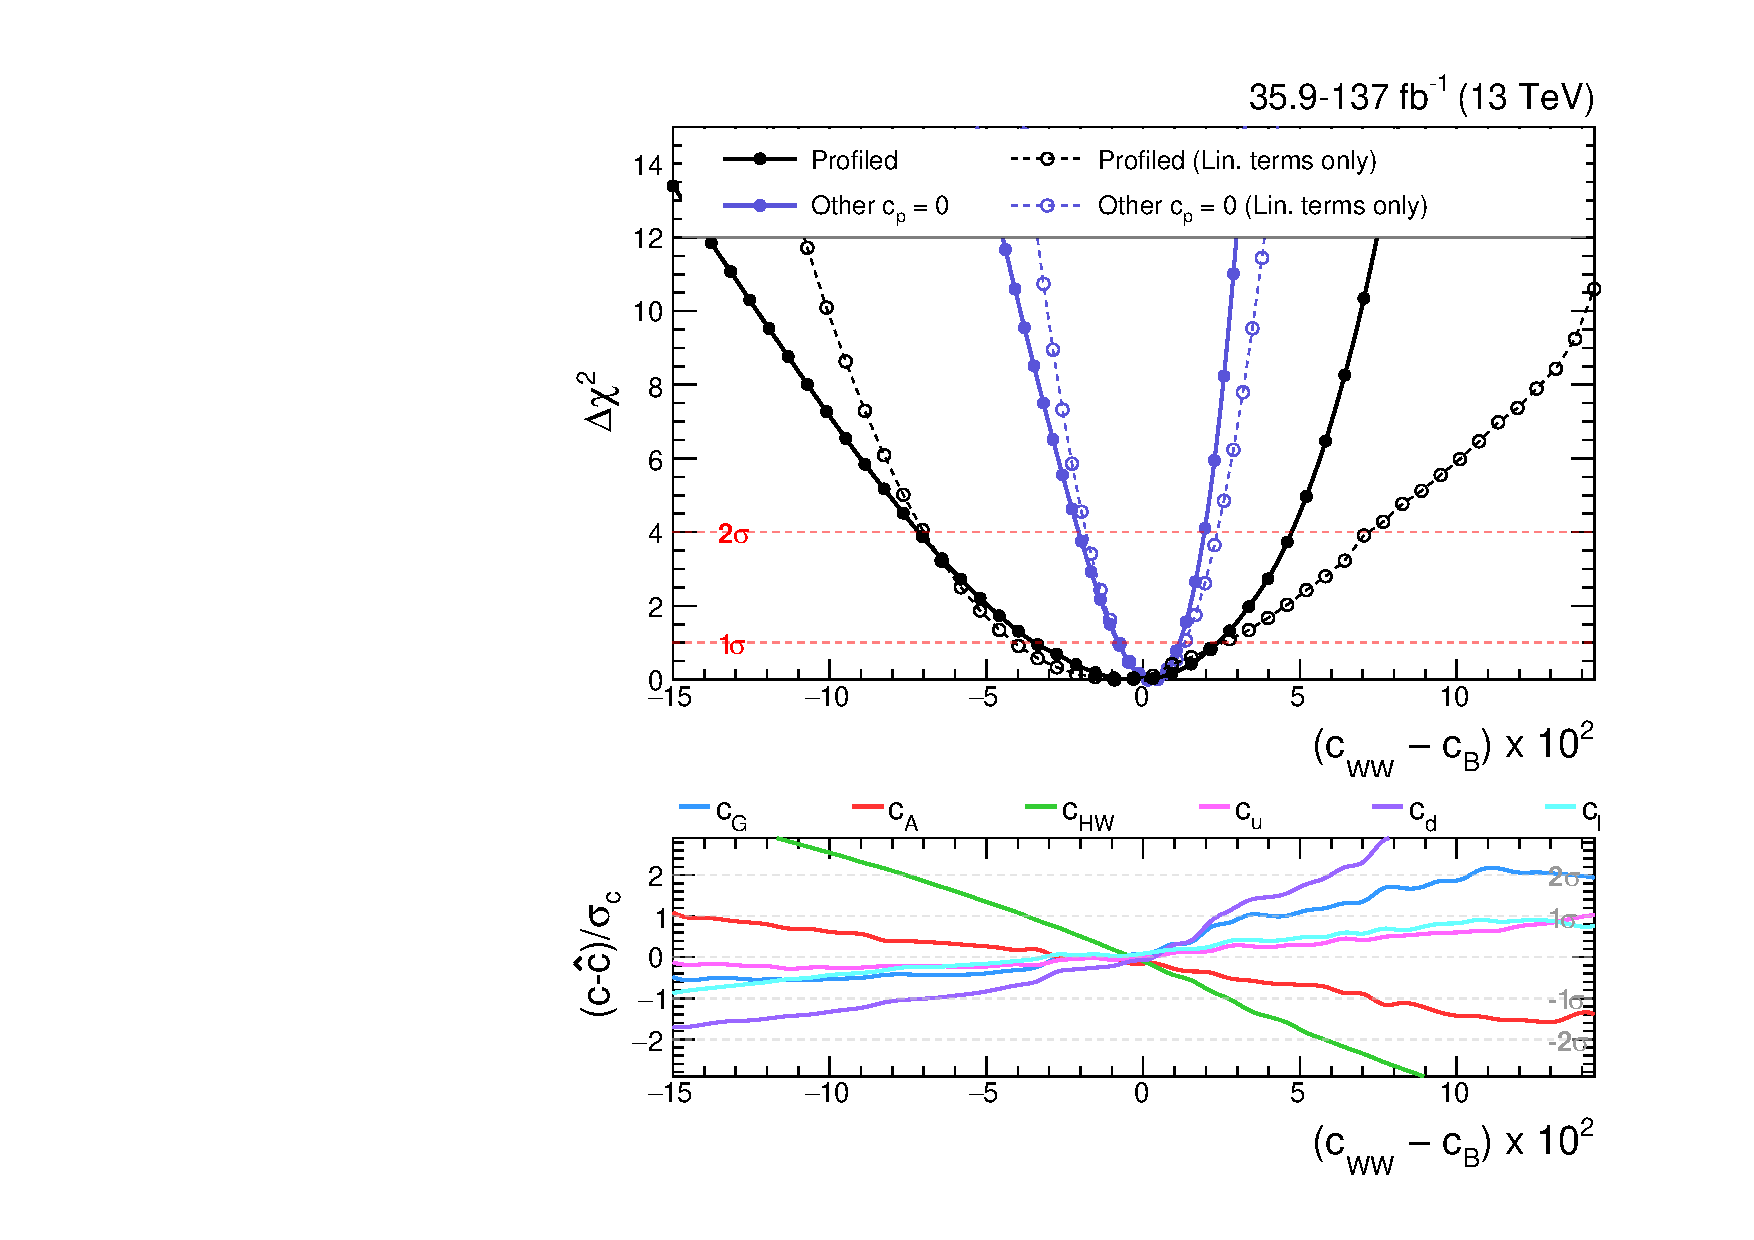
\includegraphics[width=.49\textwidth]{Figures/eft/chi2/observed/cWWMinuscB.pdf}
  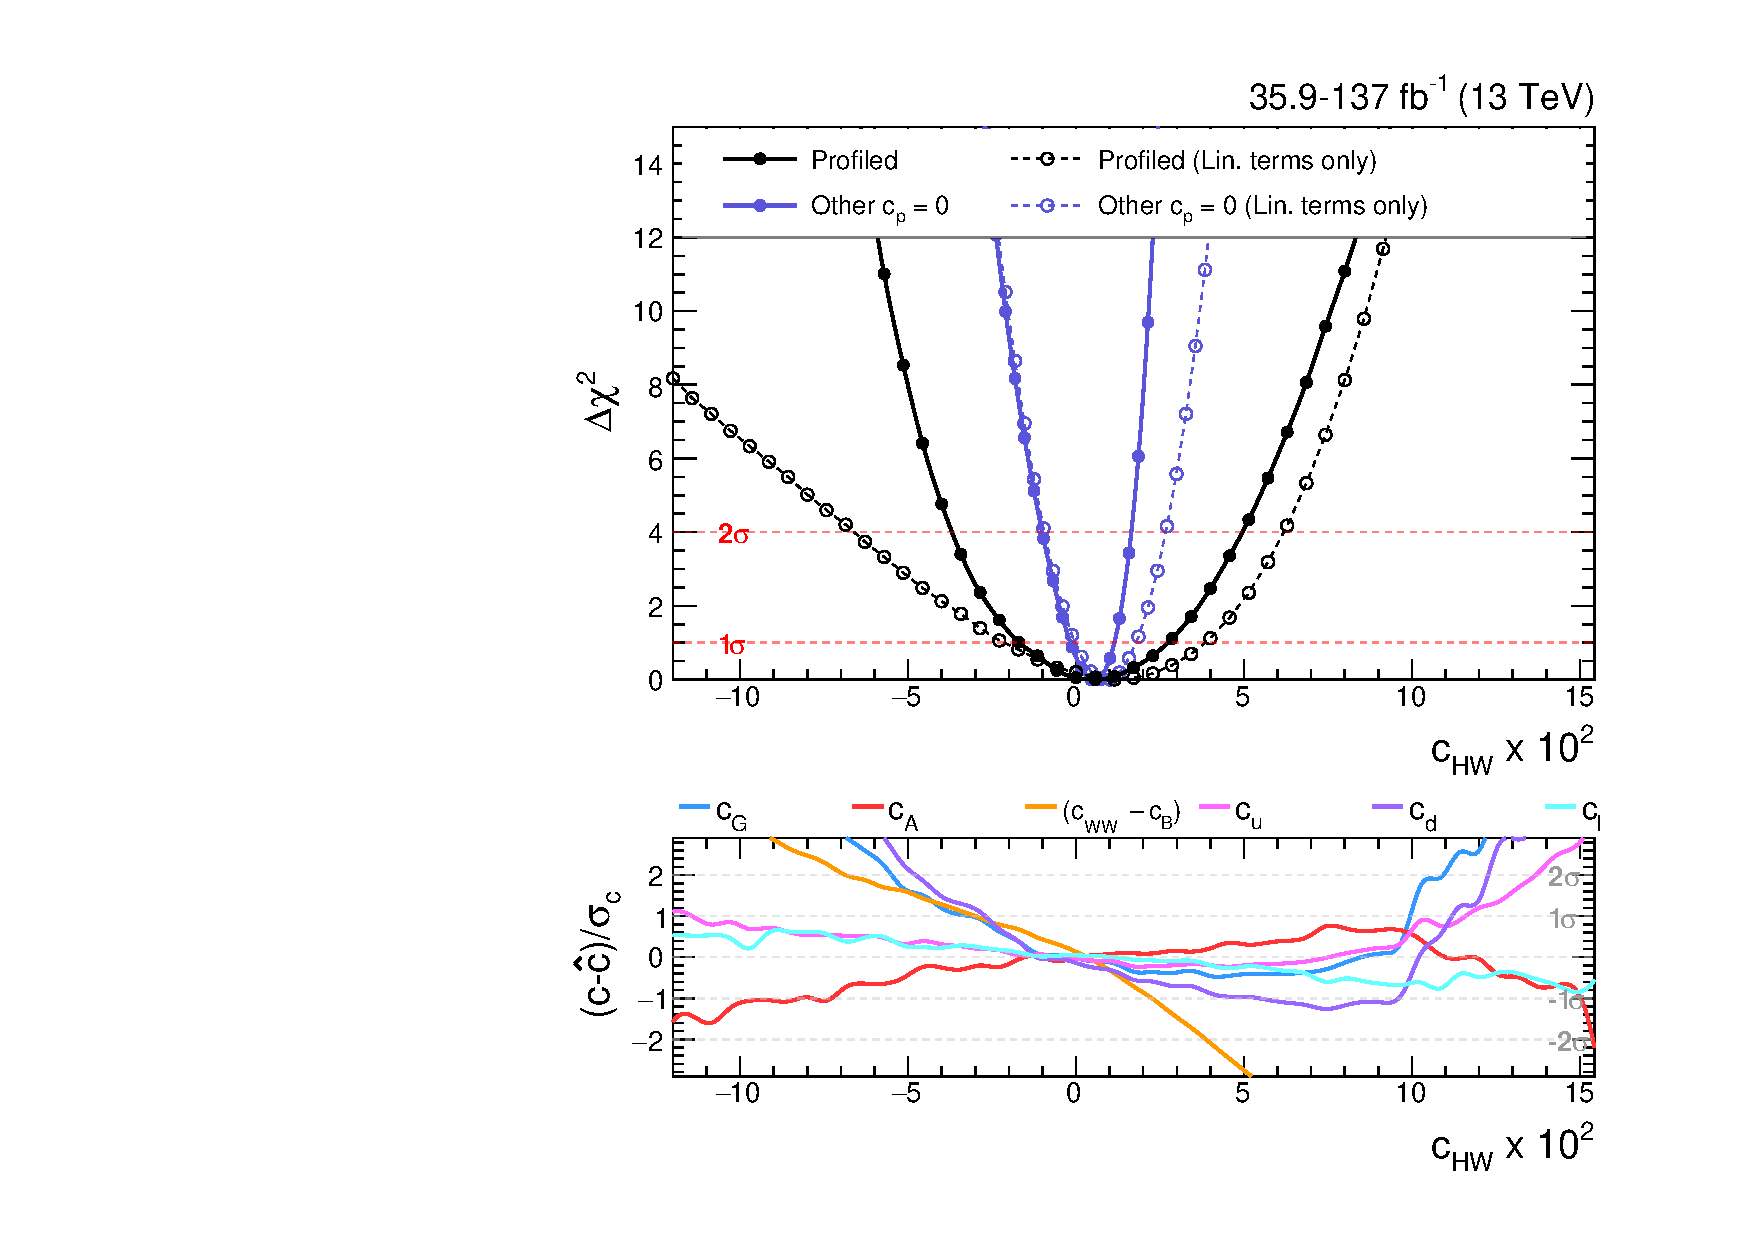
\includegraphics[width=.49\textwidth]{Figures/eft/chi2/observed/cHW.pdf}
  \caption[Simplified HEL re-interpretation: $c_G$, $c_A$, $(c_{WW}-c_B)$ and $c_{HW}$]
  {
    The $\Delta\chi^2(c_p)$ curves for the HEL parameters: $c_G$, $c_A$, $(c_{WW}-c_B)$ and $c_{HW}$. The black and purple in the top panels lines correspond to the fits in which the other parameters are profiled and fixed to the SM, respectively. The dashed lines indicate the fits when only linear terms are considered in the parametrisation. The points in each curve show the values of $c_p$ where the minimisation is performed; the lines are extracted by interpolating between these points. The horizontal red lines at $\Delta\chi^2(c_p)=1$ and 4 indicate the $1\sigma$ and $2\sigma$ confidence intervals in $c_p$, respectively. The bottom panels show the pull of the profiled parameters with respect to the parameter of interest. 
  }
  \label{fig:hel_chi2_simplified_0}
\end{figure}

% \begin{figure}[htb!]
%   \centering
% %   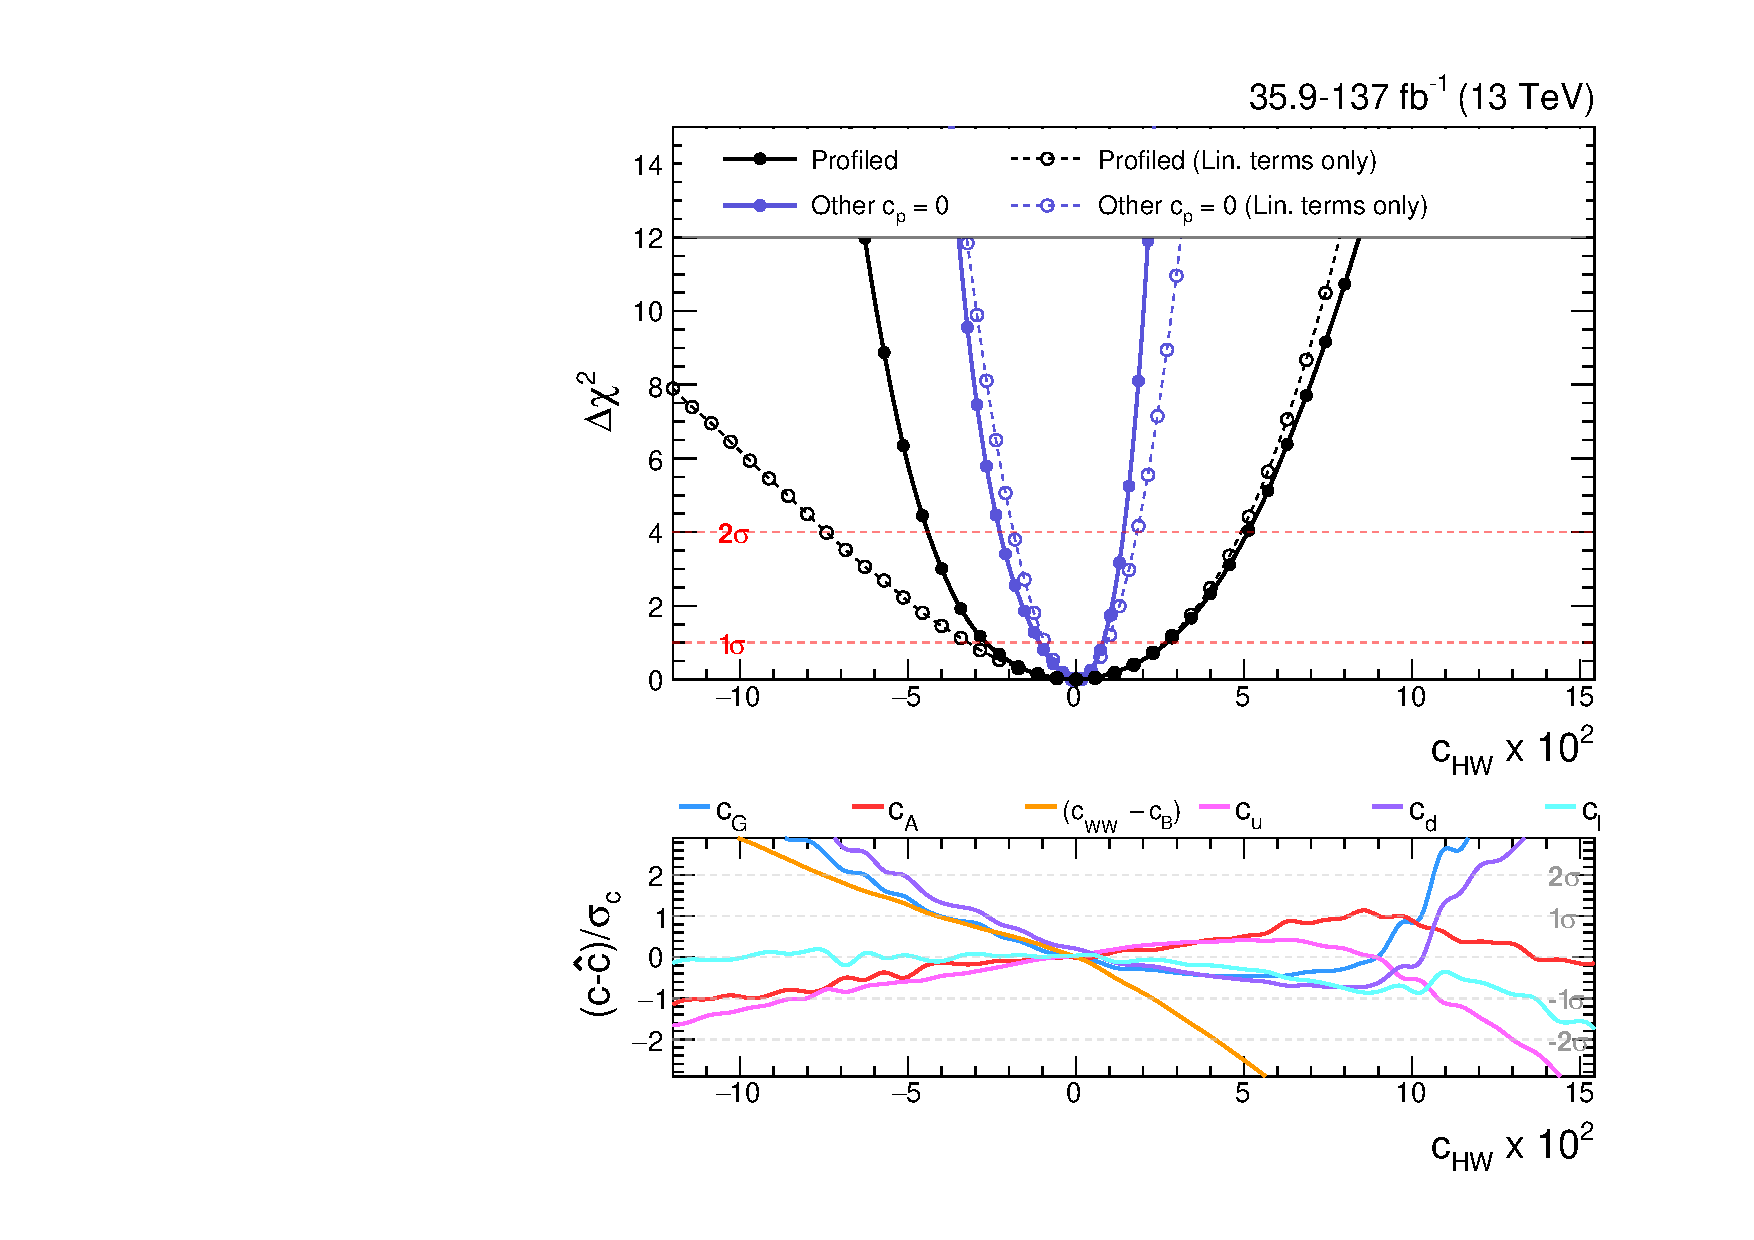
\includegraphics[width=.49\textwidth]{Figures/eft/chi2/expected/cHW.pdf}
% %   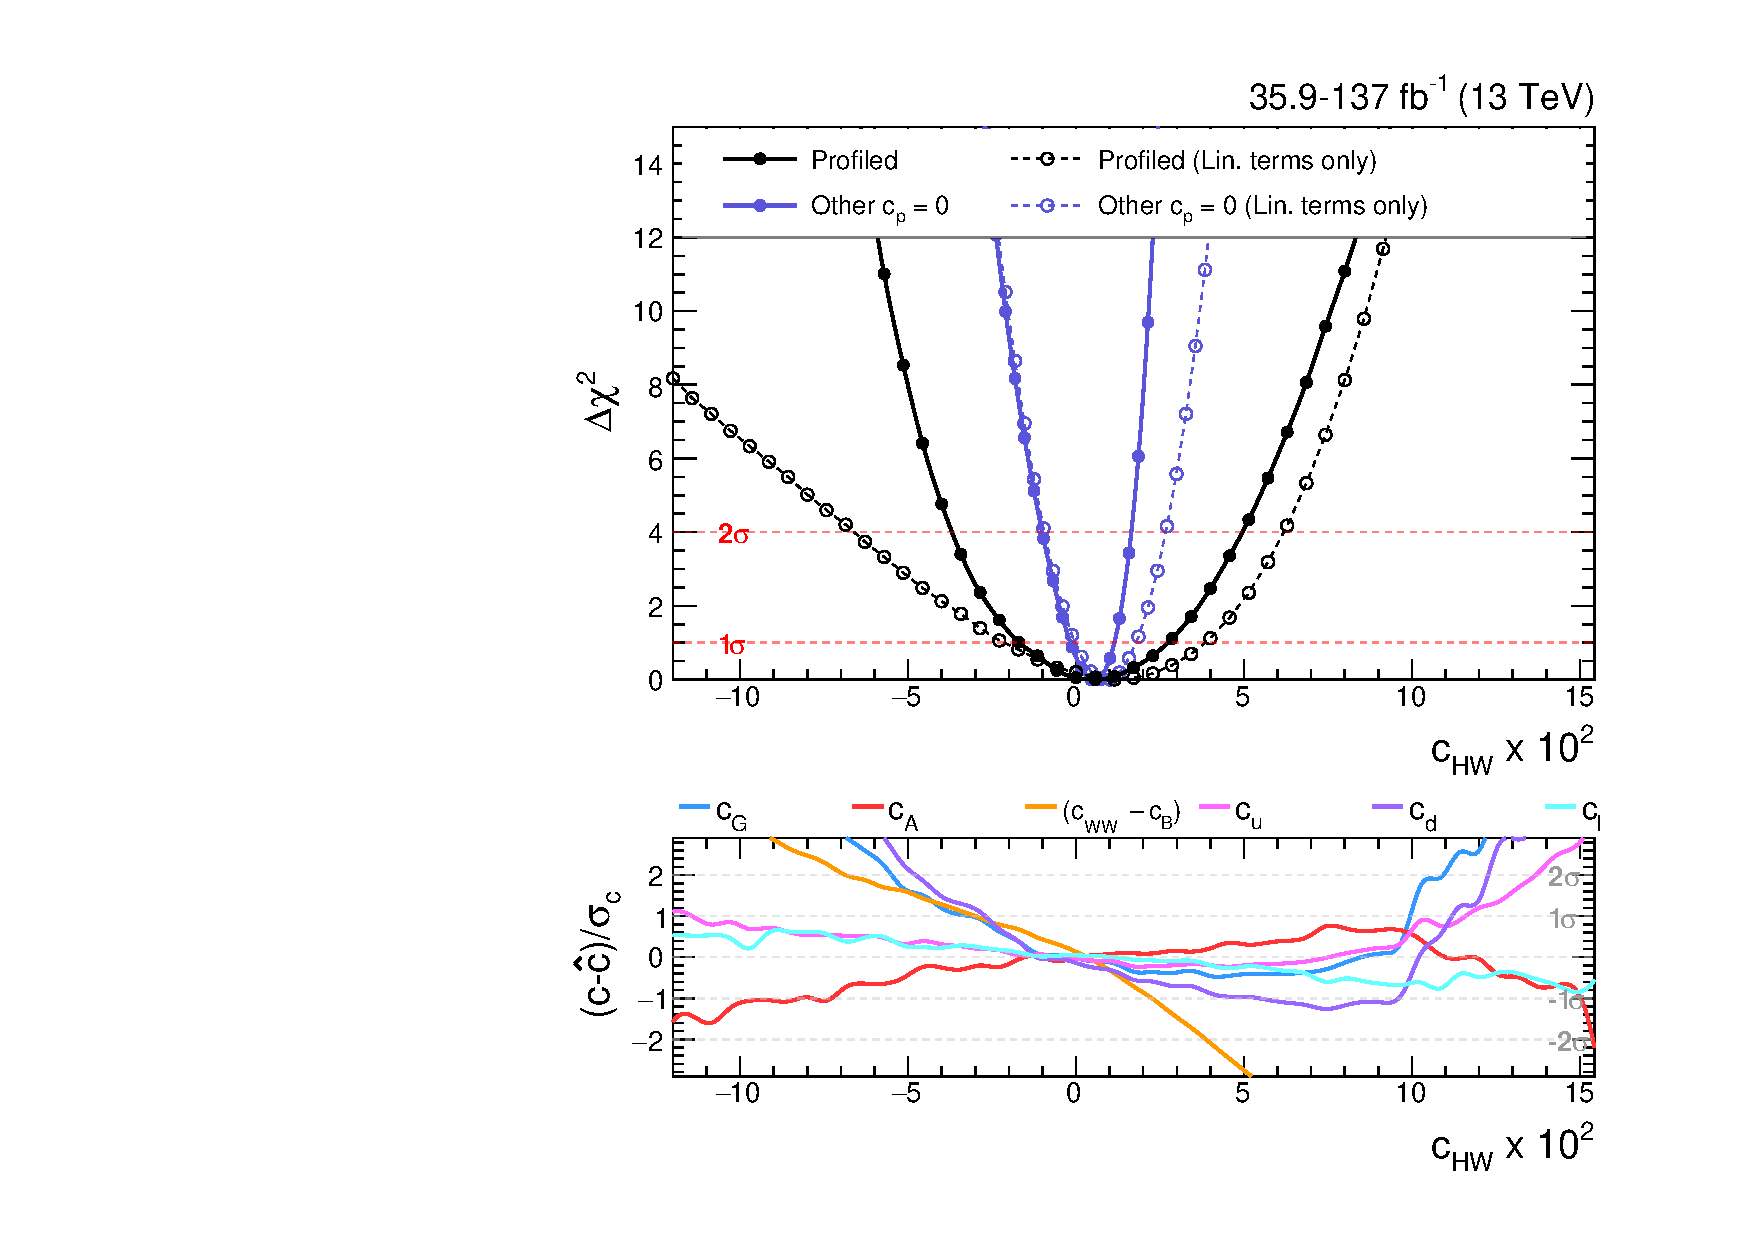
\includegraphics[width=.49\textwidth]{Figures/eft/chi2/observed/cHW.pdf}
% %   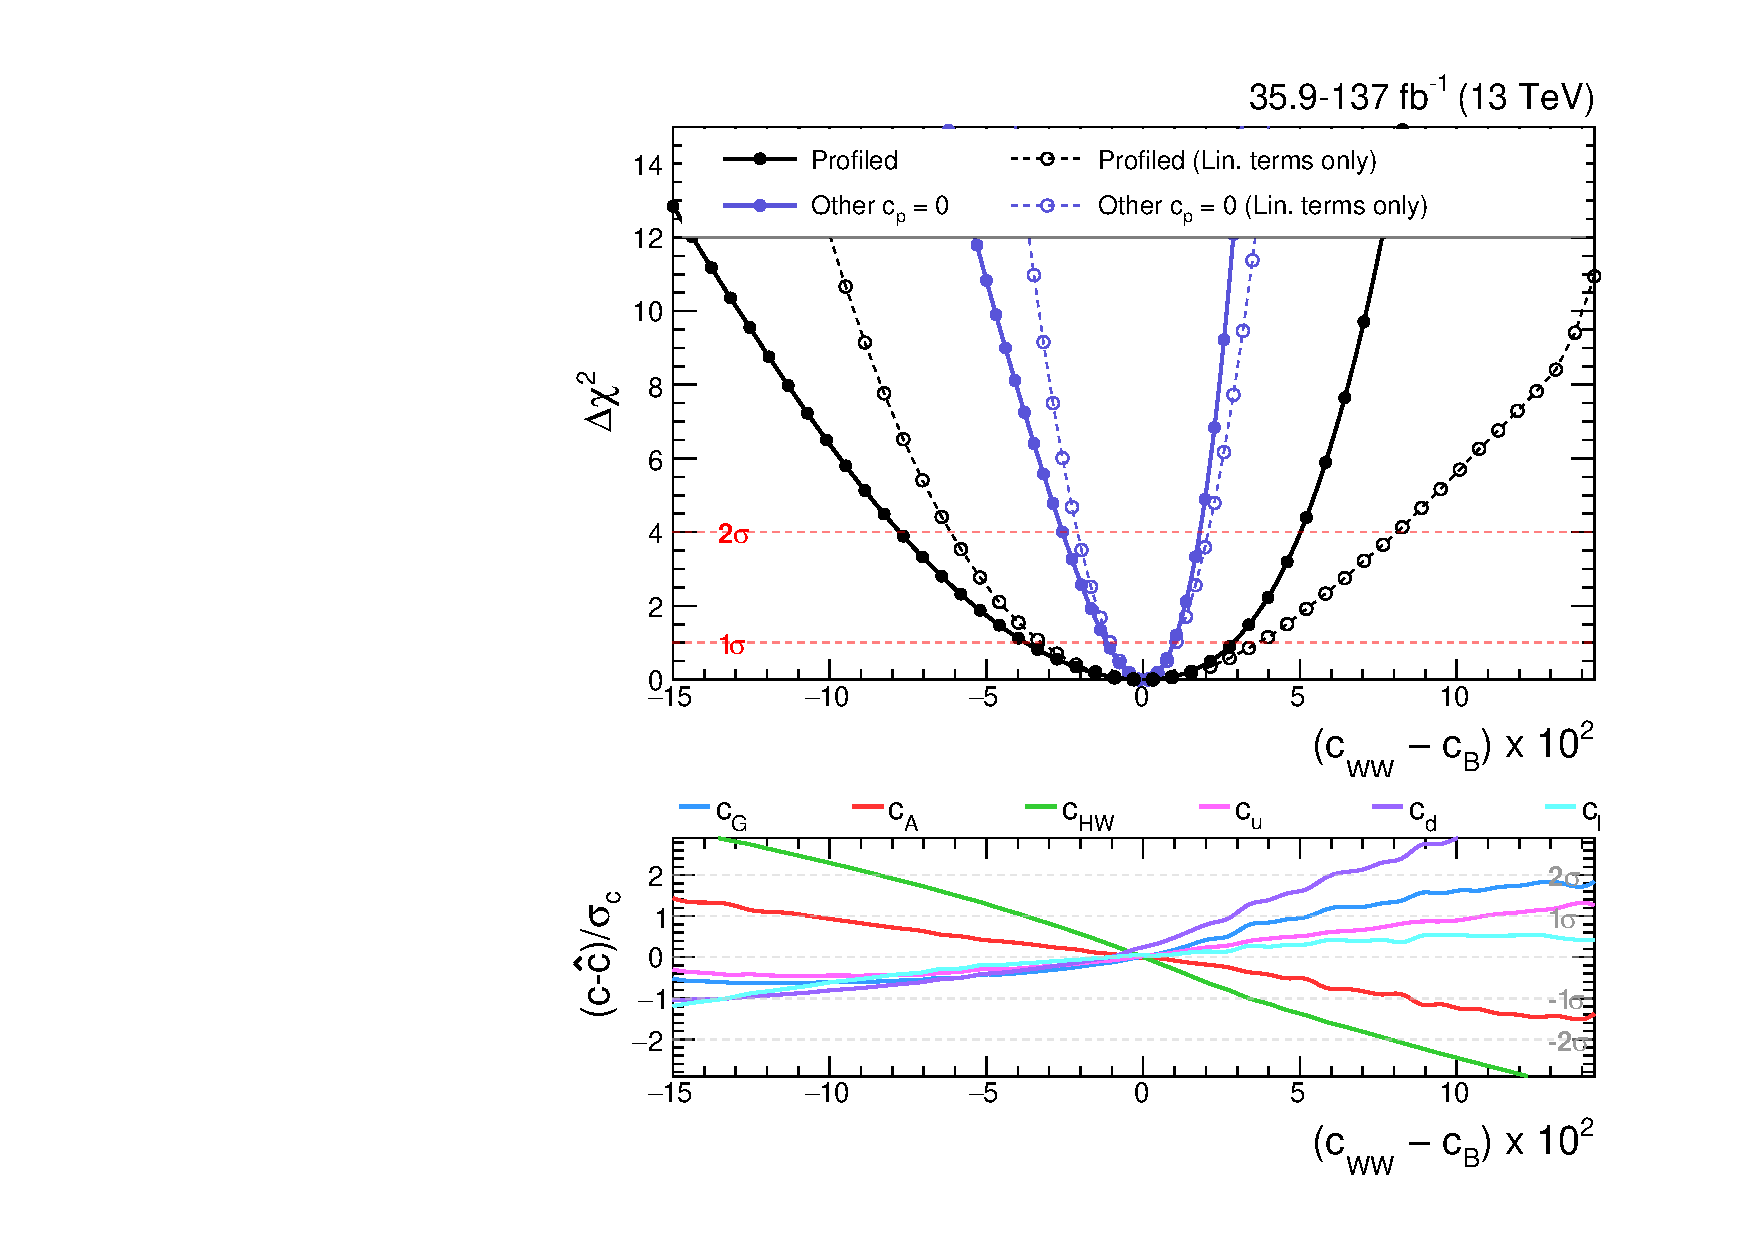
\includegraphics[width=.49\textwidth]{Figures/eft/chi2/expected/cWWMinuscB.pdf}
% %   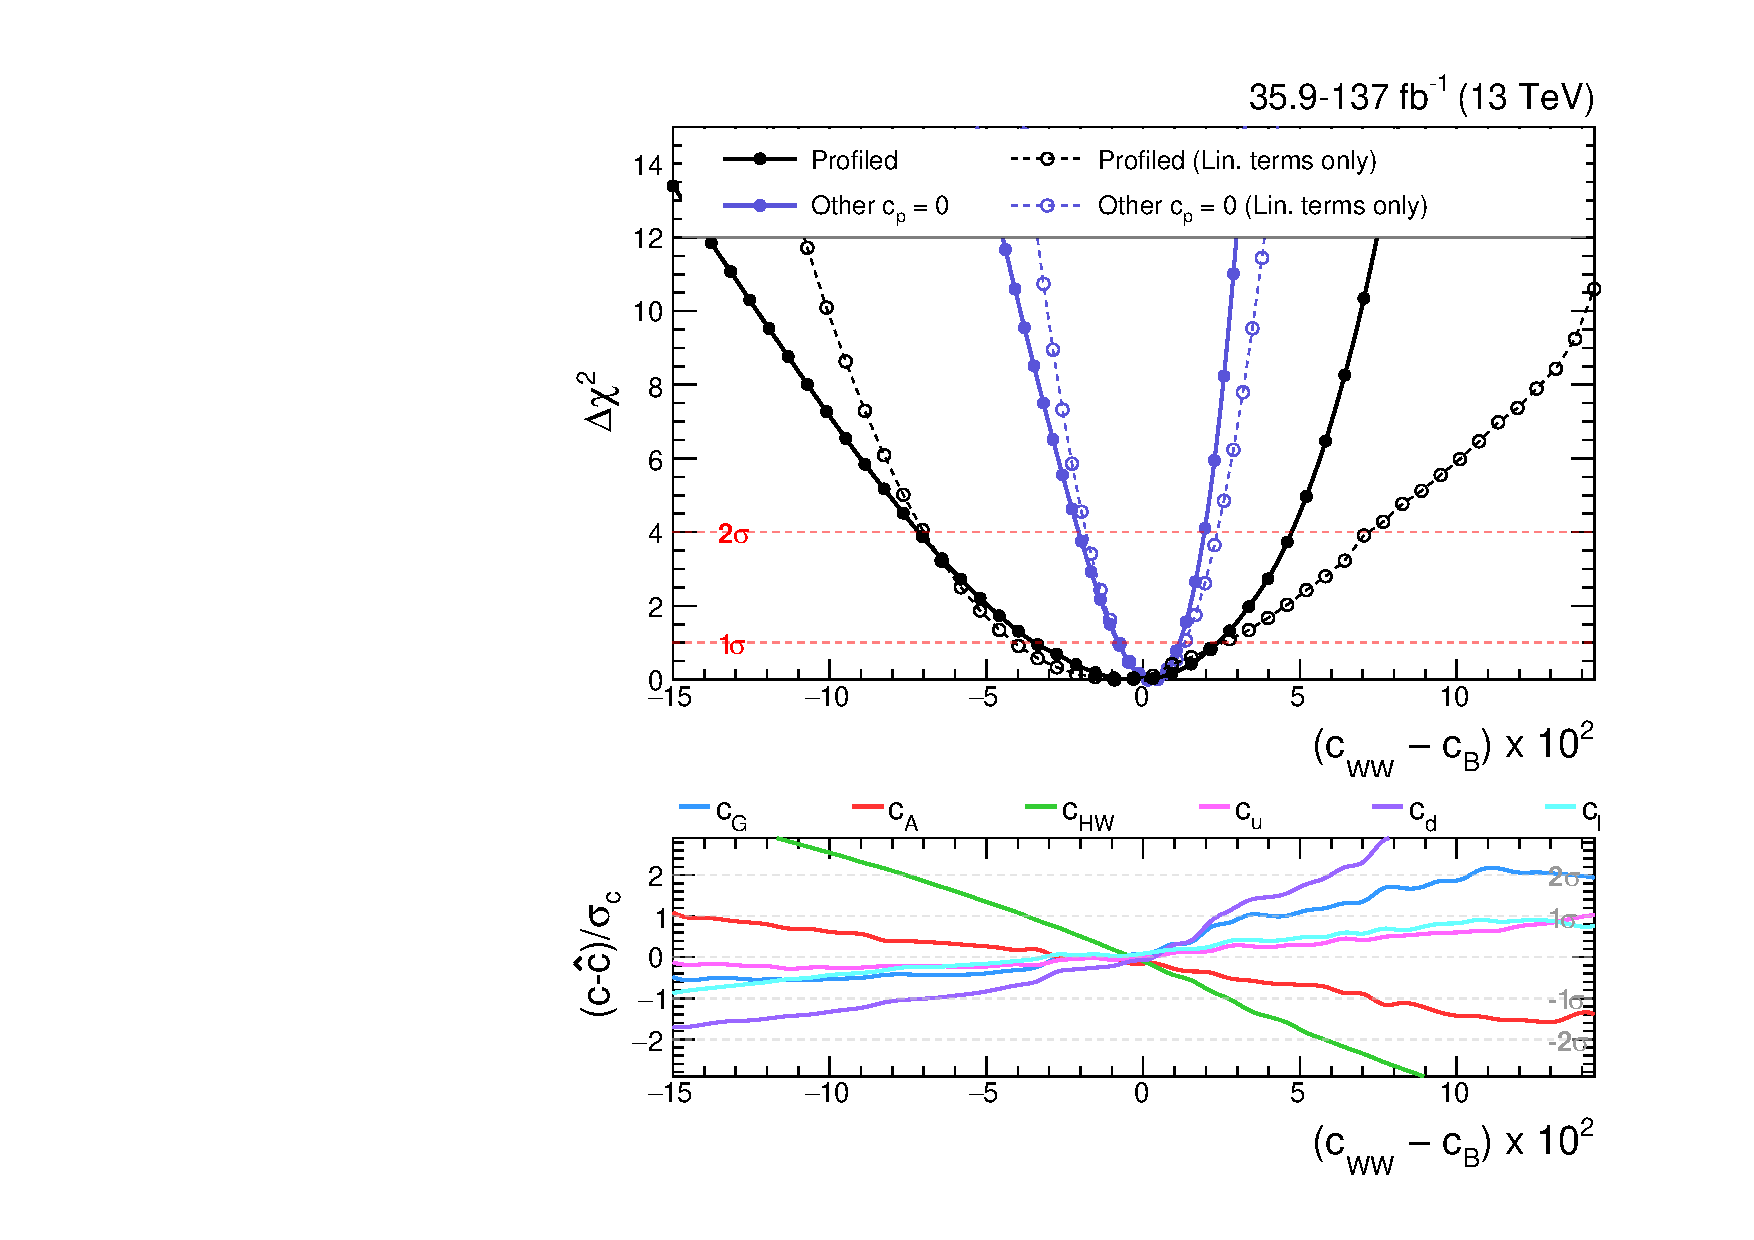
\includegraphics[width=.49\textwidth]{Figures/eft/chi2/observed/cWWMinuscB.pdf}
%   \caption[Simplified HEL re-interpretation: $(c_{WW}-c_B)$ and $c_{HW}$]
%   {
%     Add caption
%   }
%   \label{fig:hel_chi2_simplified_1}
% \end{figure}

\begin{figure}[htb!]
  \centering
%   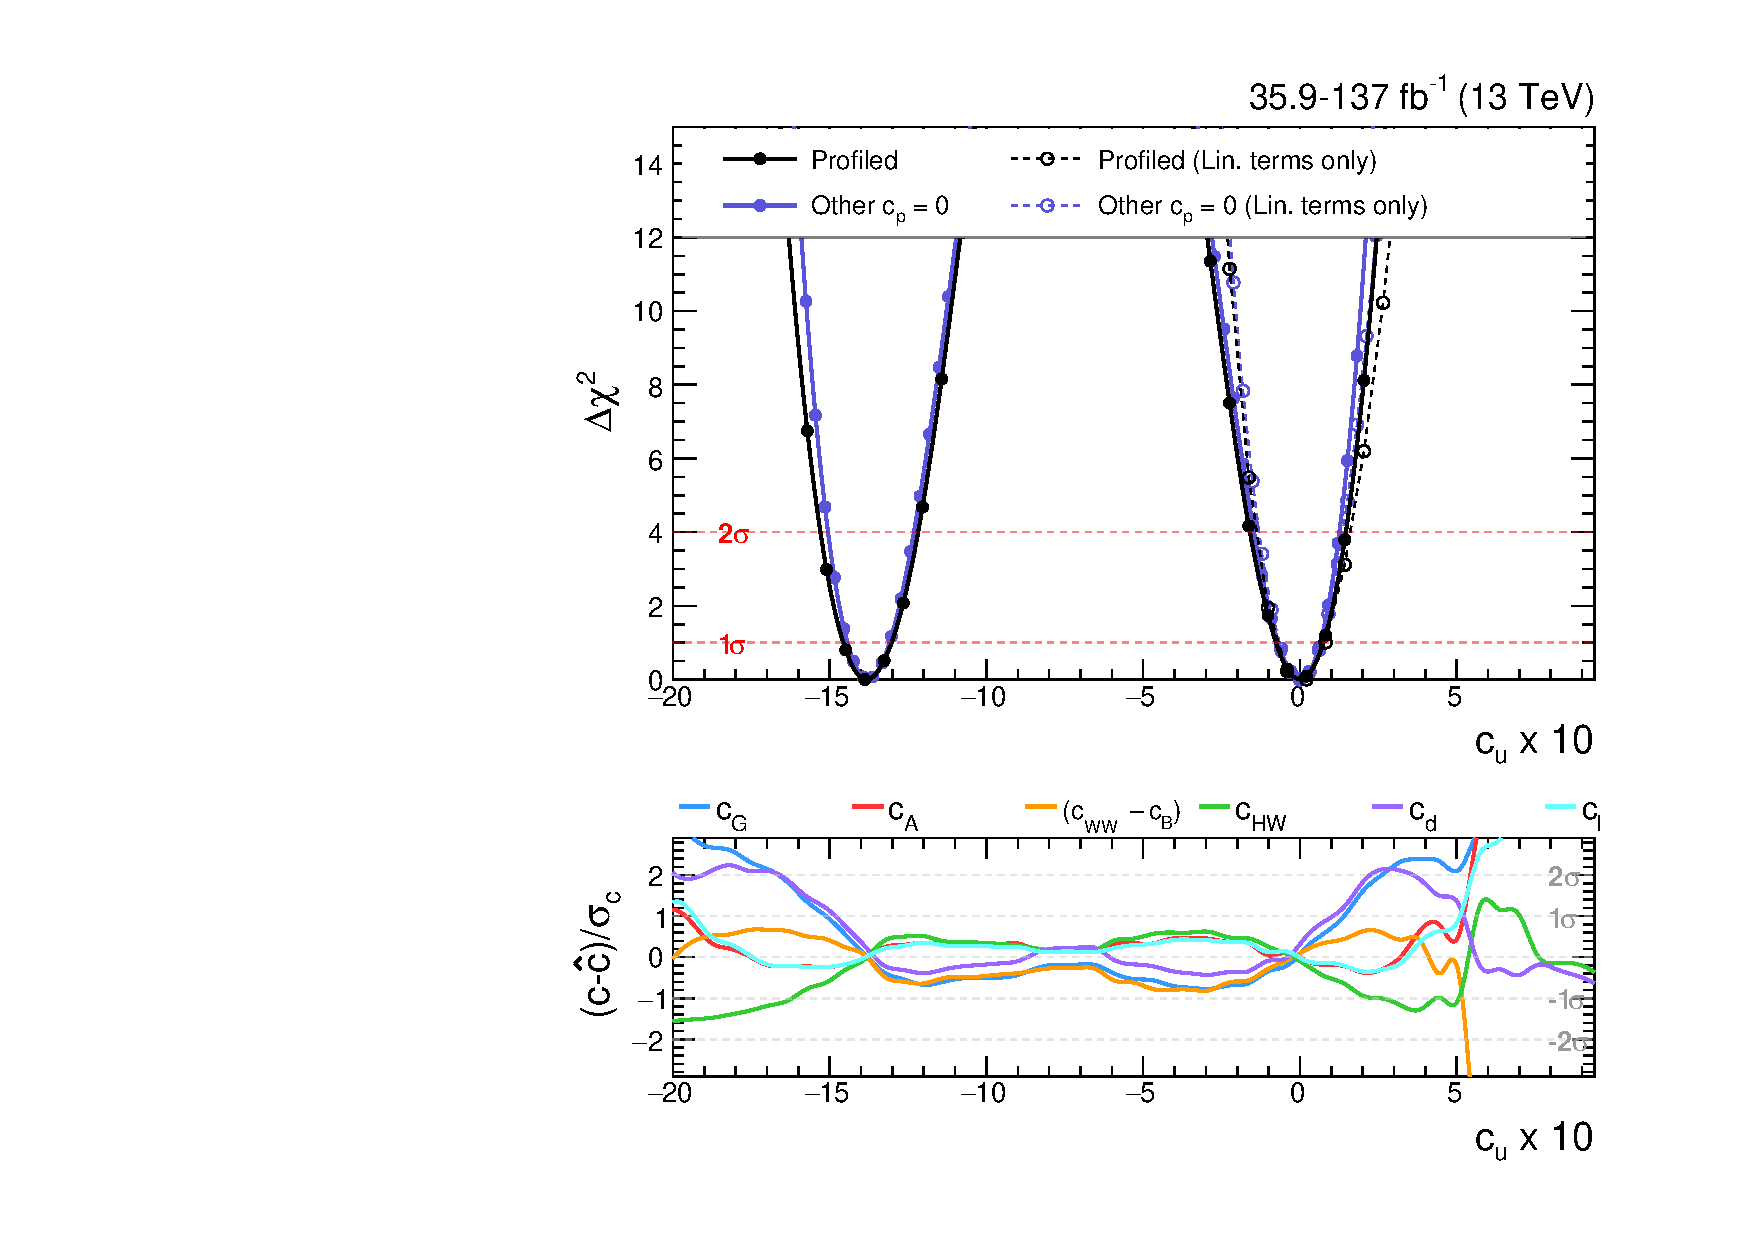
\includegraphics[width=.49\textwidth]{Figures/eft/chi2/expected/cu.pdf}
  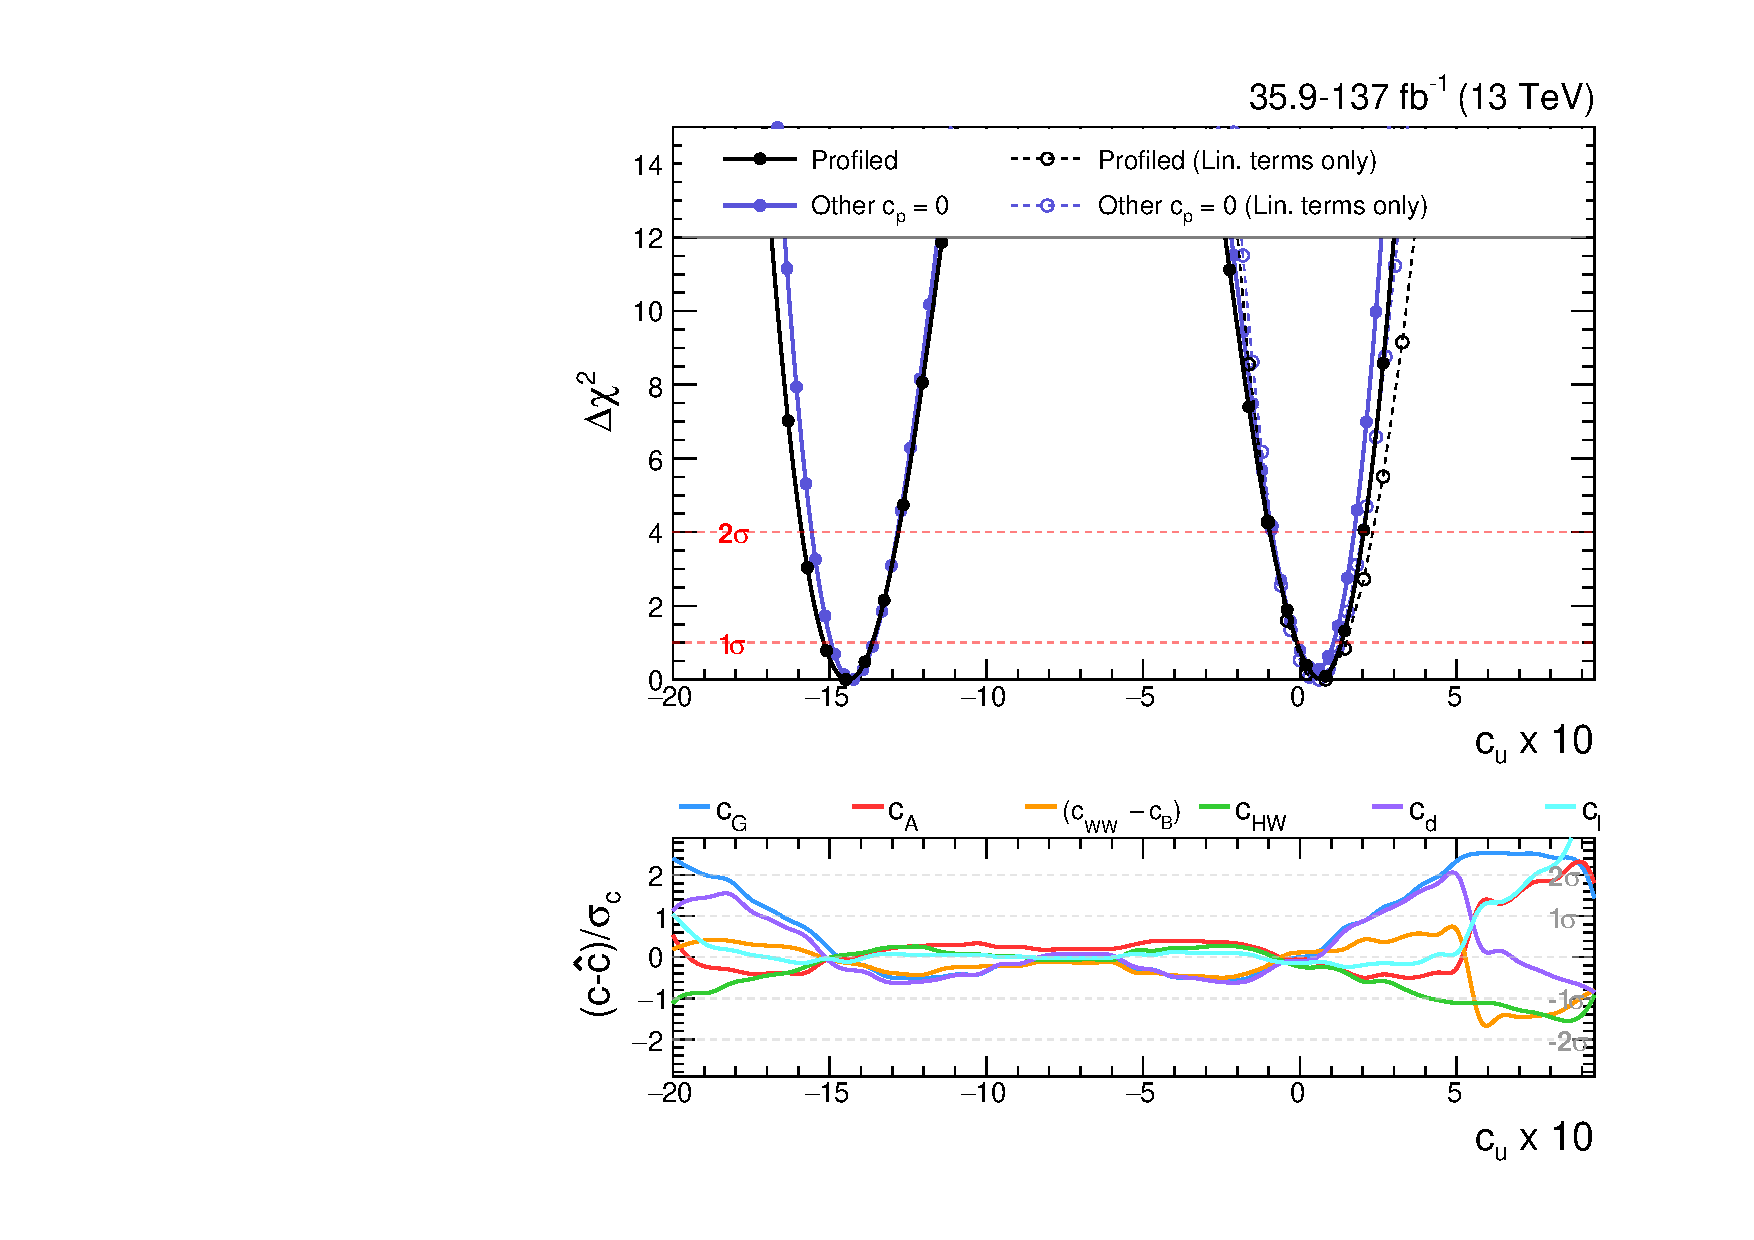
\includegraphics[width=.49\textwidth]{Figures/eft/chi2/observed/cu.pdf}
%   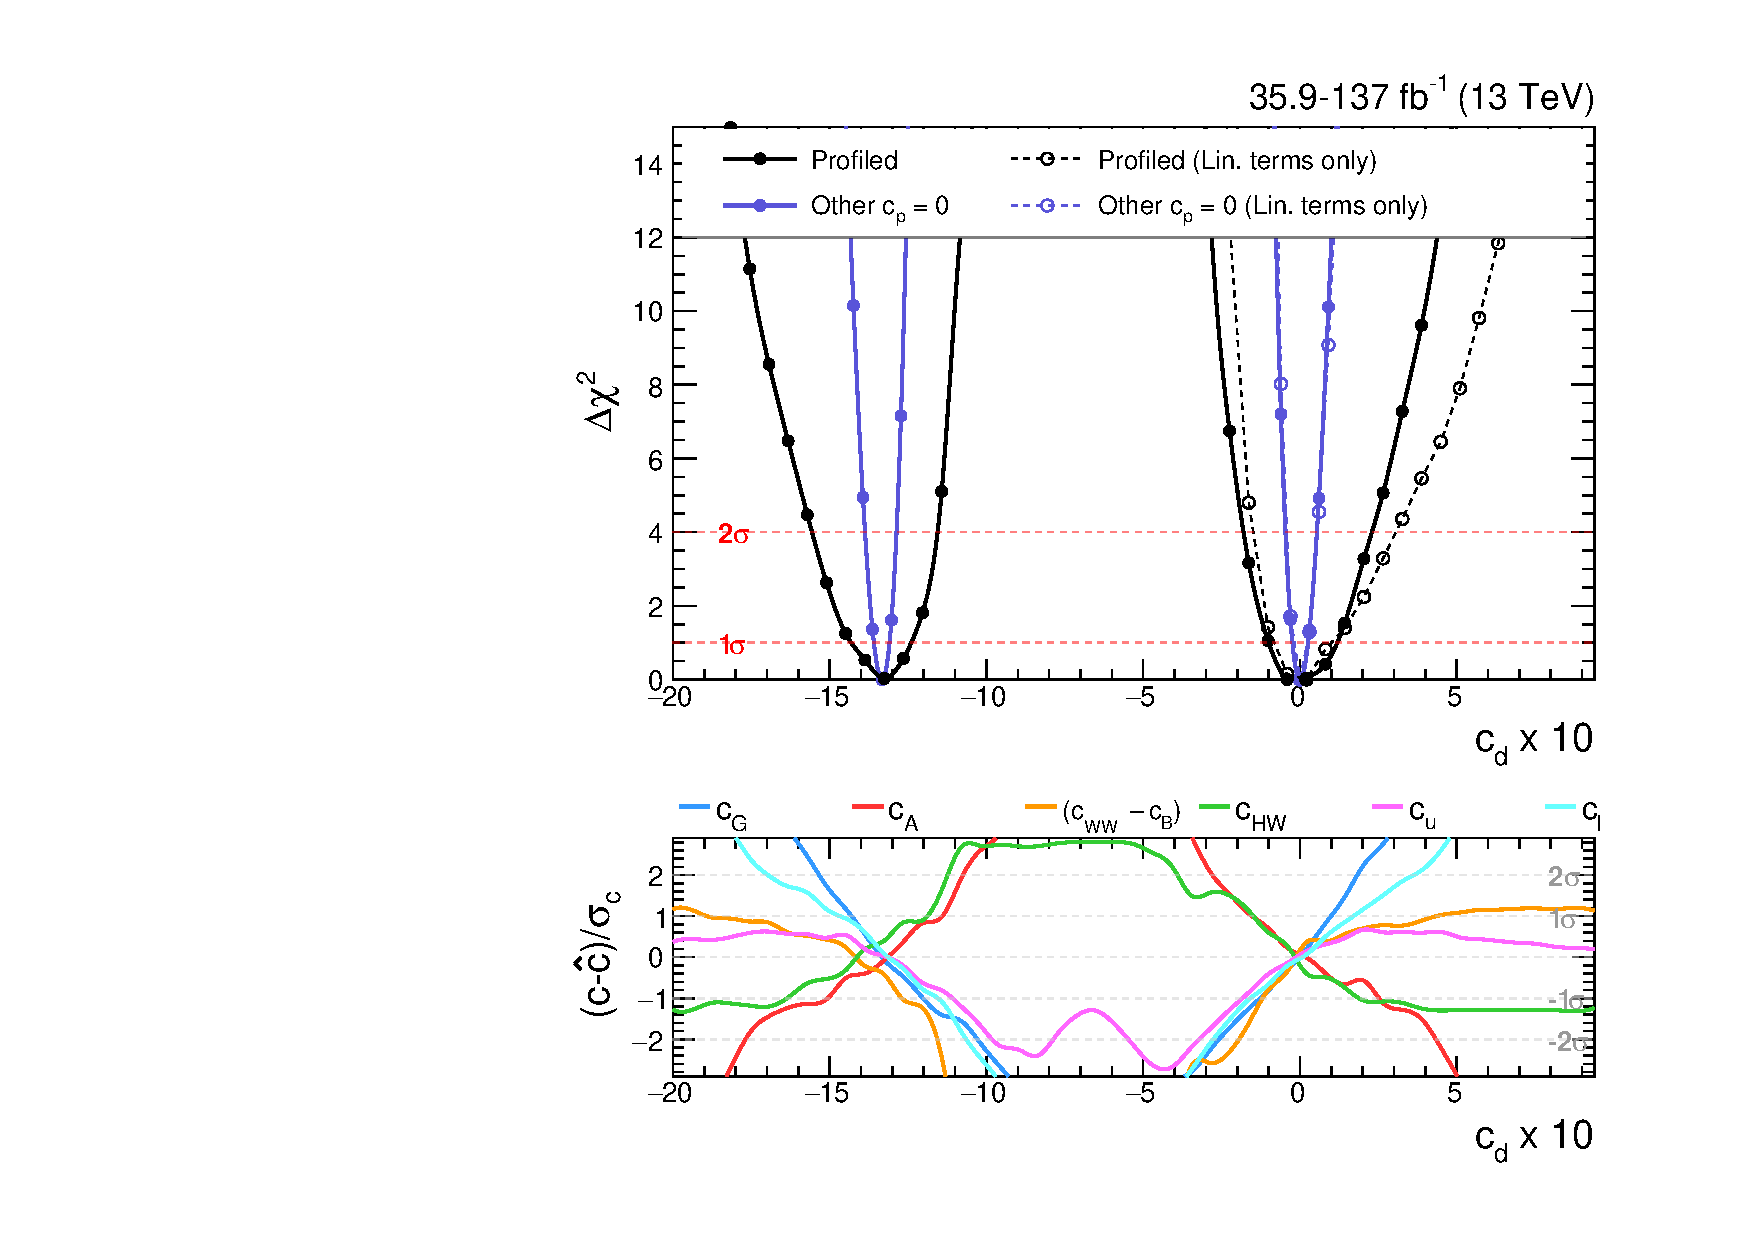
\includegraphics[width=.49\textwidth]{Figures/eft/chi2/expected/cd.pdf}
  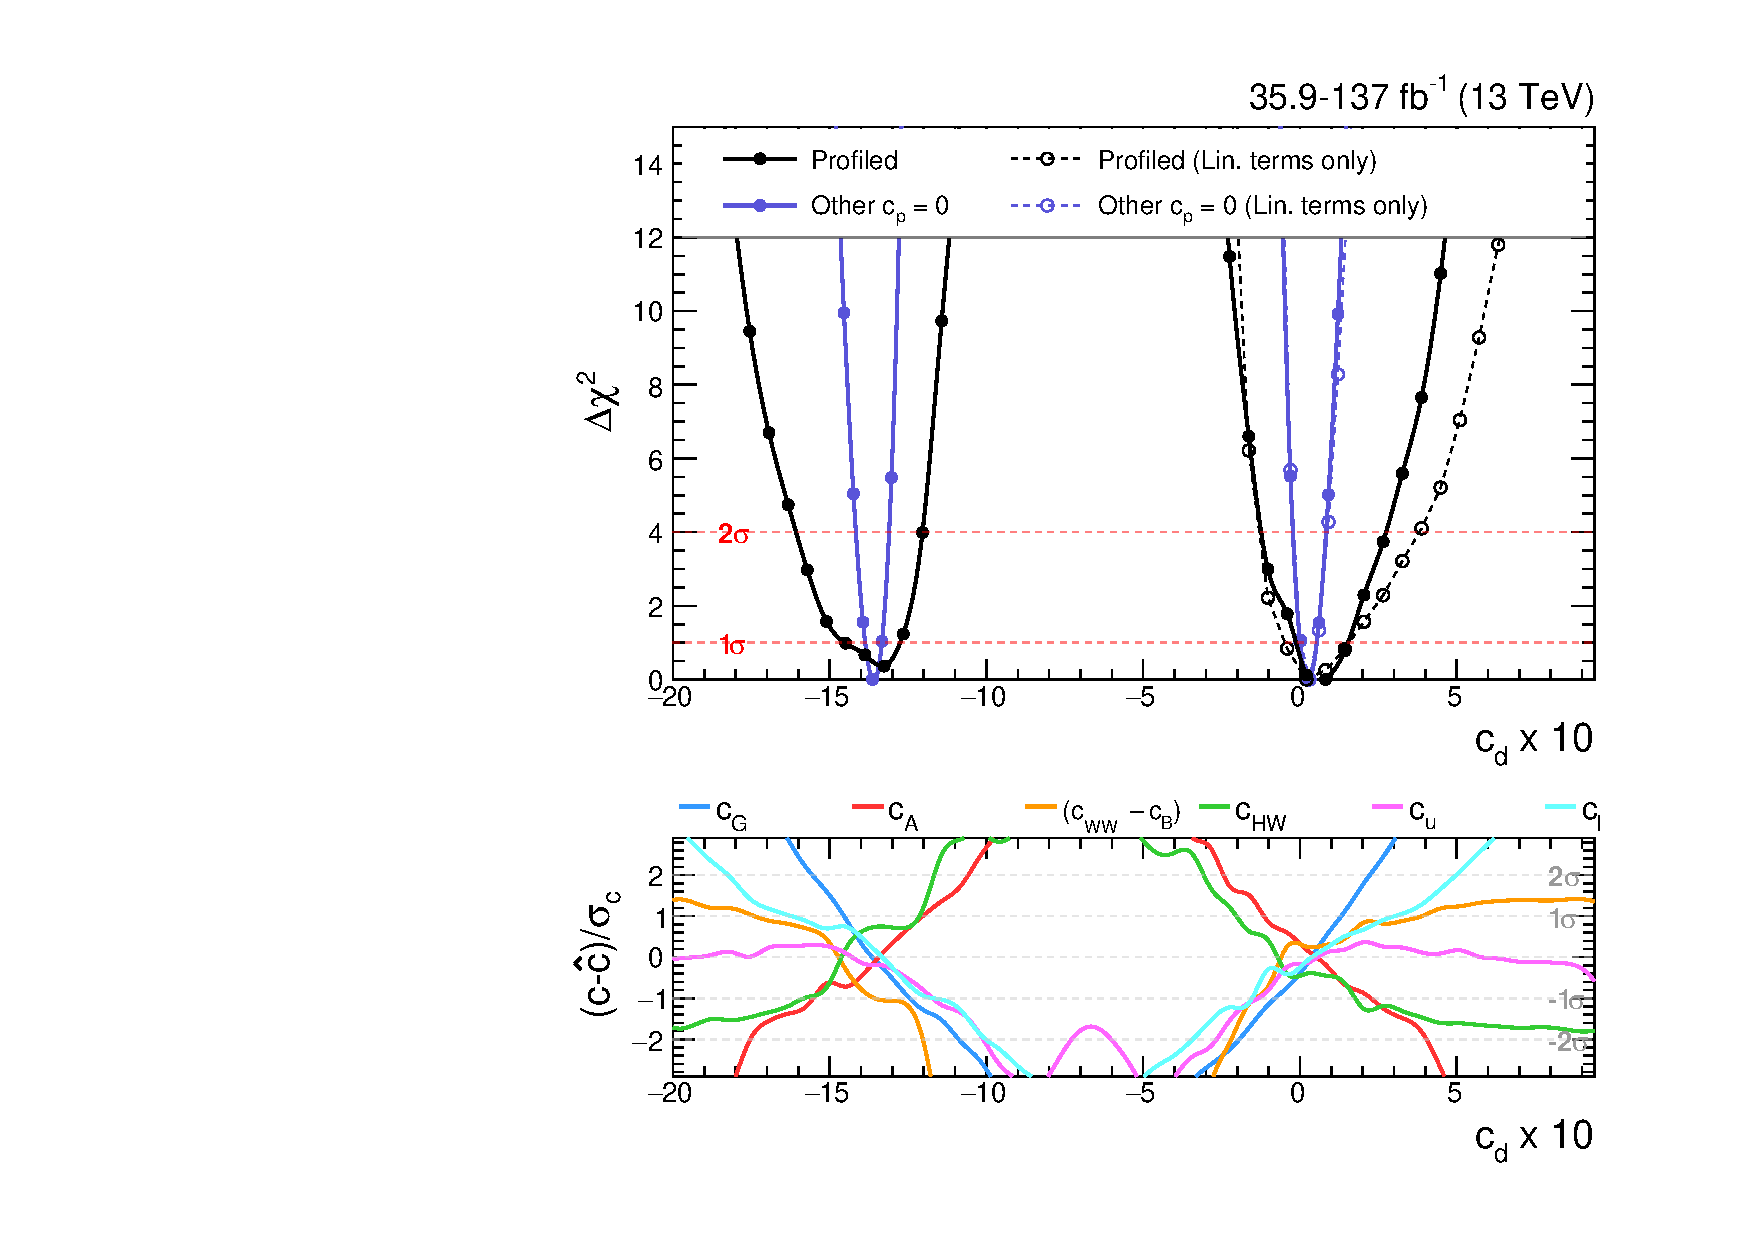
\includegraphics[width=.49\textwidth]{Figures/eft/chi2/observed/cd.pdf}
%   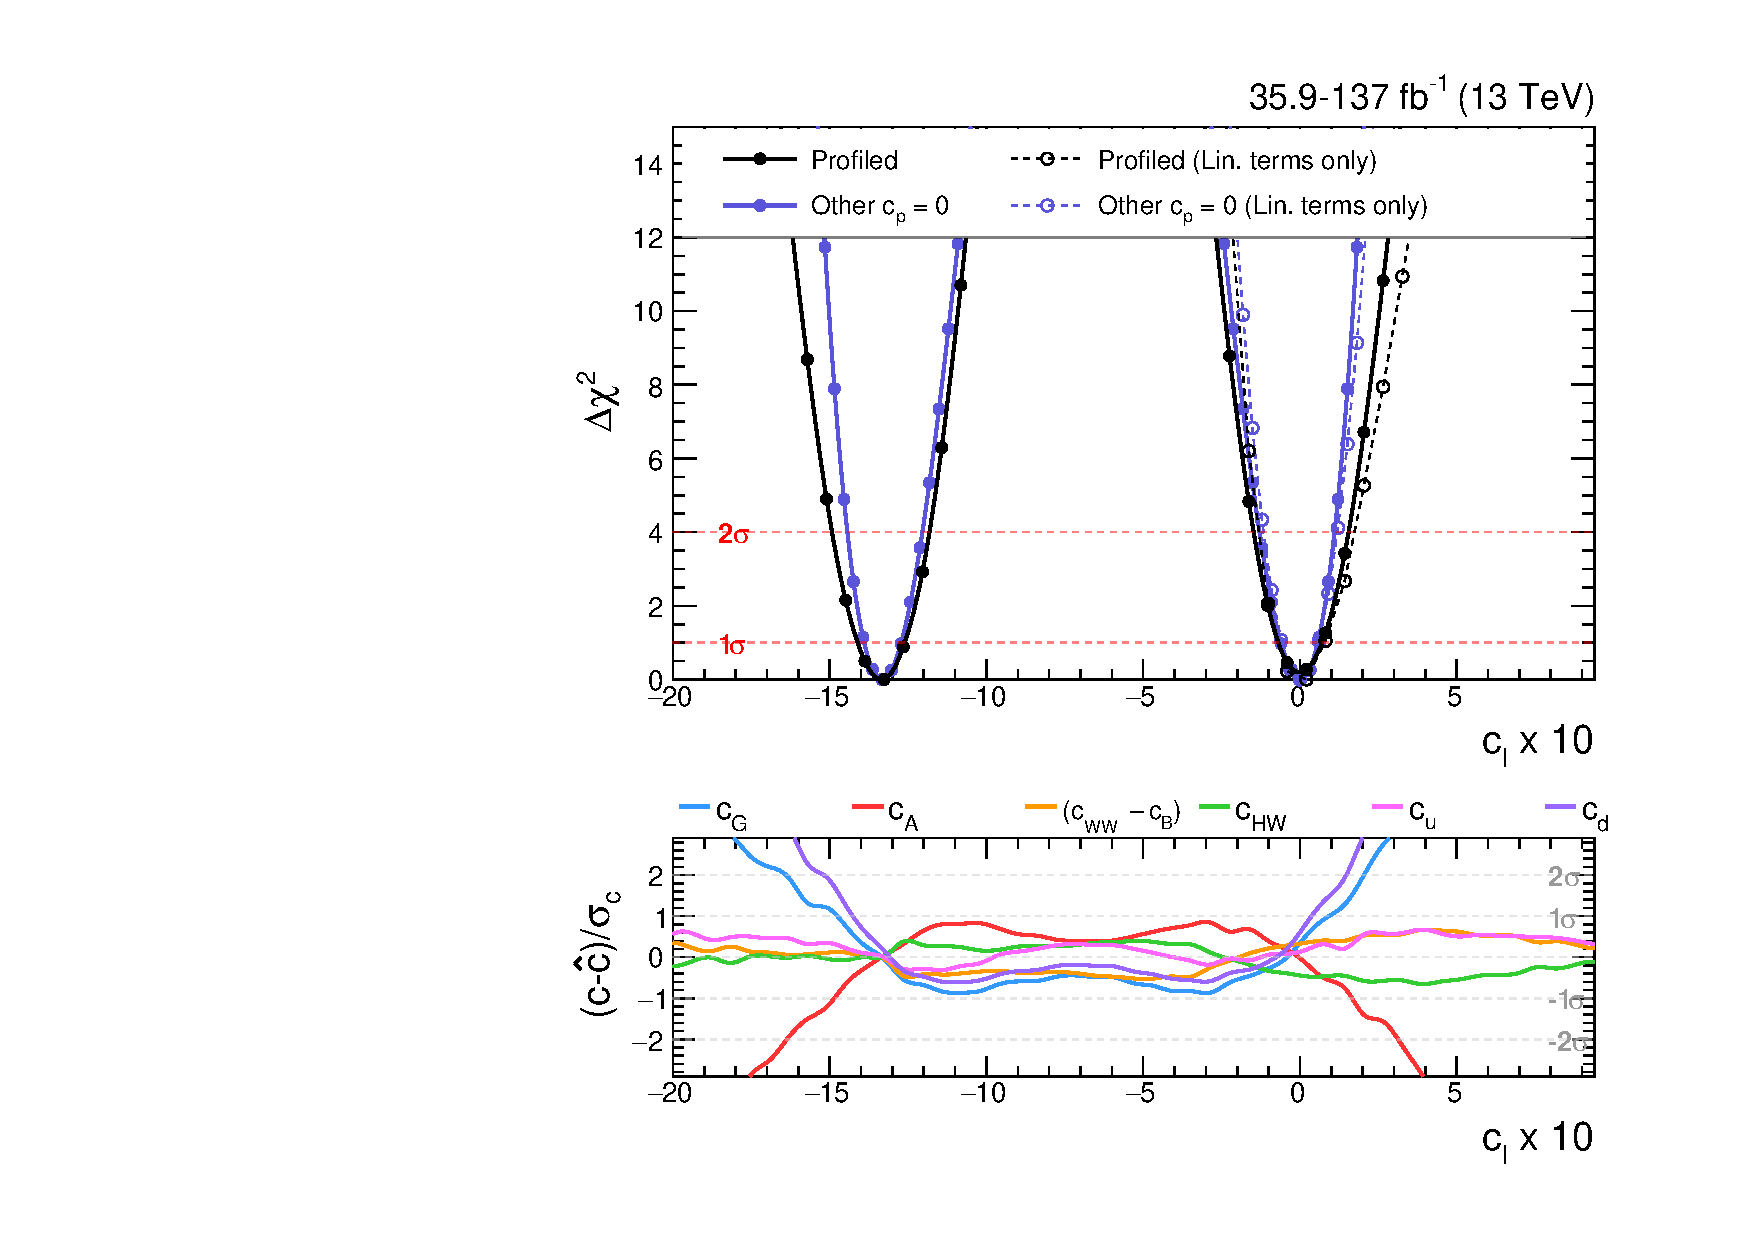
\includegraphics[width=.49\textwidth]{Figures/eft/chi2/expected/cl.pdf}
  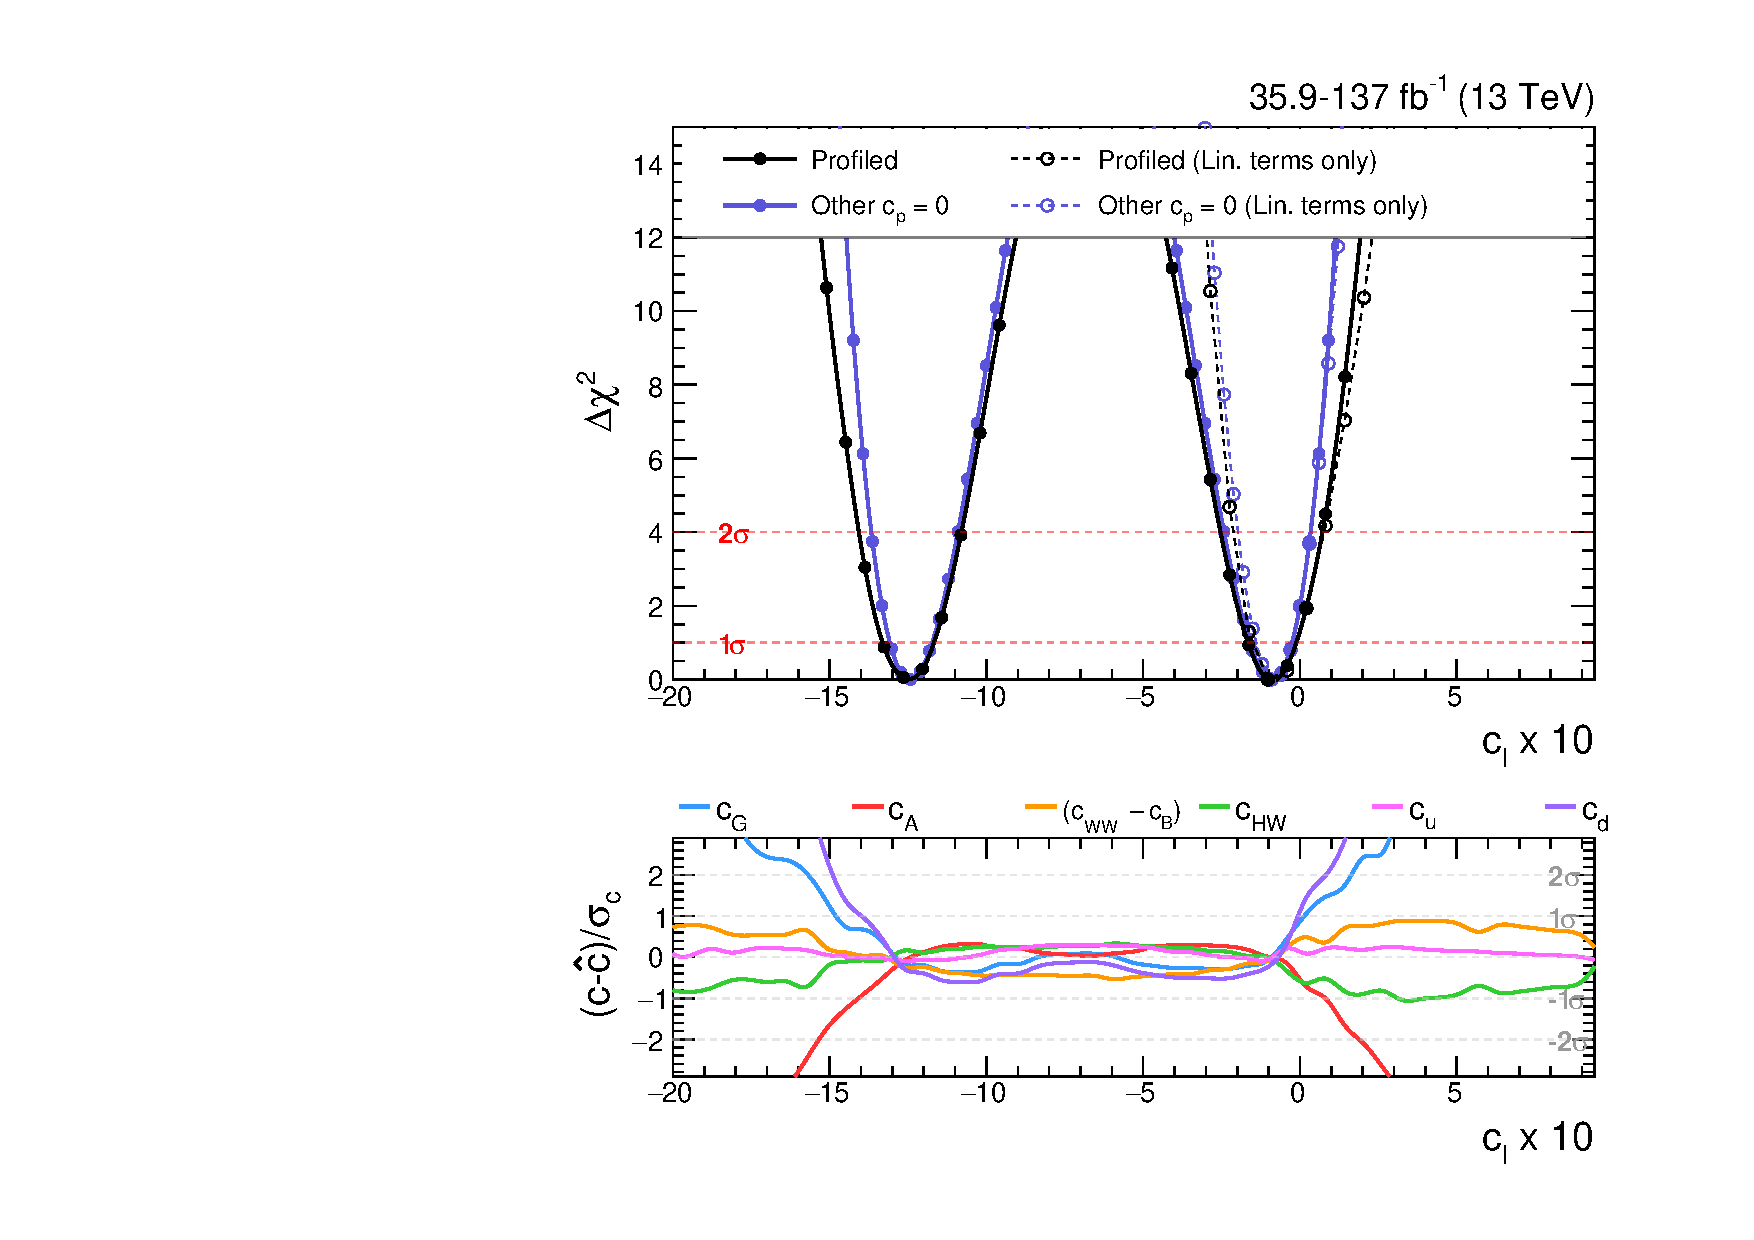
\includegraphics[width=.49\textwidth]{Figures/eft/chi2/observed/cl.pdf}
  \caption[Simplified HEL re-interpretation: $c_u$, $c_d$ and $c_{\ell}$]
  {
    The $\Delta\chi^2(c_p)$ curves for the HEL parameters: $c_u$, $c_d$ and $c_\ell$. The black and purple lines in the top panels correspond to the fits in which the other parameters are profiled and fixed to the SM, respectively. The dashed lines indicate the fits when only linear terms are considered in the parametrisation. The points in each curve show the values of $c_p$ where the minimisation is performed; the lines are extracted by interpolating between these points. The horizontal red lines at $\Delta\chi^2(c_p)=1$ and 4 indicate the $1\sigma$ and $2\sigma$ confidence intervals in $c_p$, respectively. The bottom panels show the pull of the profiled parameters with respect to the parameter of interest. 
  }
  \label{fig:hel_chi2_simplified_1}
\end{figure}

\FloatBarrier
\newpage
\section{Full likelihood results and discussion}\label{sec:eft_results}
This section presents the results using the full combination likelihood, according to the results extraction procedure detailed in section \ref{sec:results_extraction}. Performing the interpretation in this way is unique to experiments, in the sense that no assumptions are made about the nature of the likelihood surface, and all correlations between input analyses are accounted for. The theoretical uncertainties in the SM predictions of the cross sections and branching fractions ($\vec{\theta}^{\,\rm{th}}_{s}$) are directly folded into the measurement. Uncertainties in the HEL parametrisation, namely the uncertainties in the $A_p$ and $B_{pr}$ prefactors arising from missing higher order corrections and limited MC statistics are neglected. Furthermore, the bbH, tH and ggZH processes are fixed to their SM predictions in the fit, within theoretical uncertainties. This reflects the fact that there are no dedicated analysis categories targeting such production modes in the combination; although conservative this ensures there is no gain in constraining power from production modes that are not explicitly probed.

Figure \ref{fig:hel_likelihood_scans} shows the resulting $q(c_p)$ curves. Two likelihood scans are performed for each of the seven HEL parameters following the same scenarios used in section \ref{sec:hel_simplified_cms}. The first scenario, represented by the dashed lines, corresponds to considering BSM effects in a single EFT operator, such that the other HEL parameters are fixed to 0 in the scan. The second scenario considers BSM effects in all HEL parameters simultaneously, and is shown by the solid lines. In practice, this is performed by scanning over the parameter of interest and profiling the other HEL parameters in the minimisation. As expected, the constraints are tighter for the first scenario, however the act of setting the other HEL parameters to zero introduces a higher degree of model dependence into the measurement. In all fits, the HEL parameters have been scaled by a constant multiplier as the minimiser is more stable for parameters of order 1.

\begin{figure}[htbp]
  \centering
  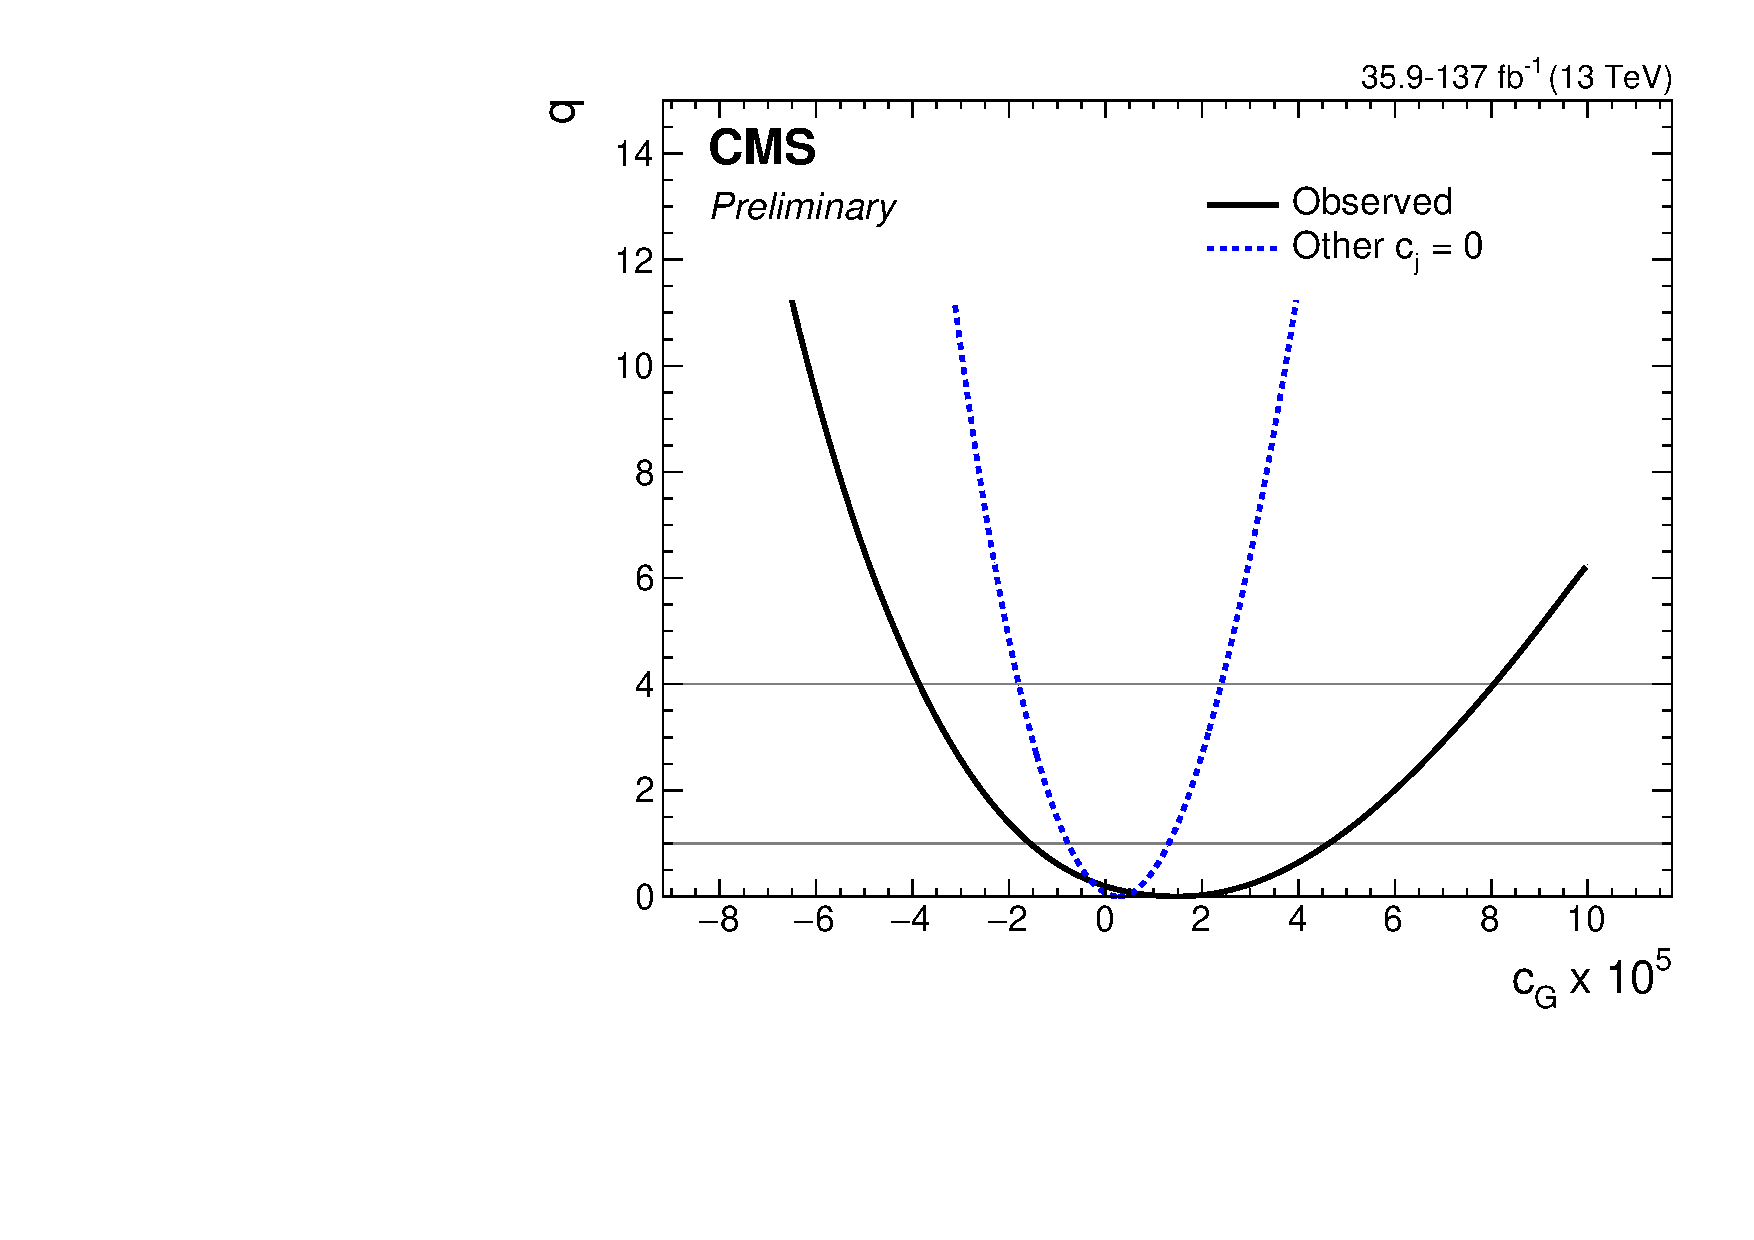
\includegraphics[width=.42\linewidth]{Figures/eft/cG_likelihood.pdf}
  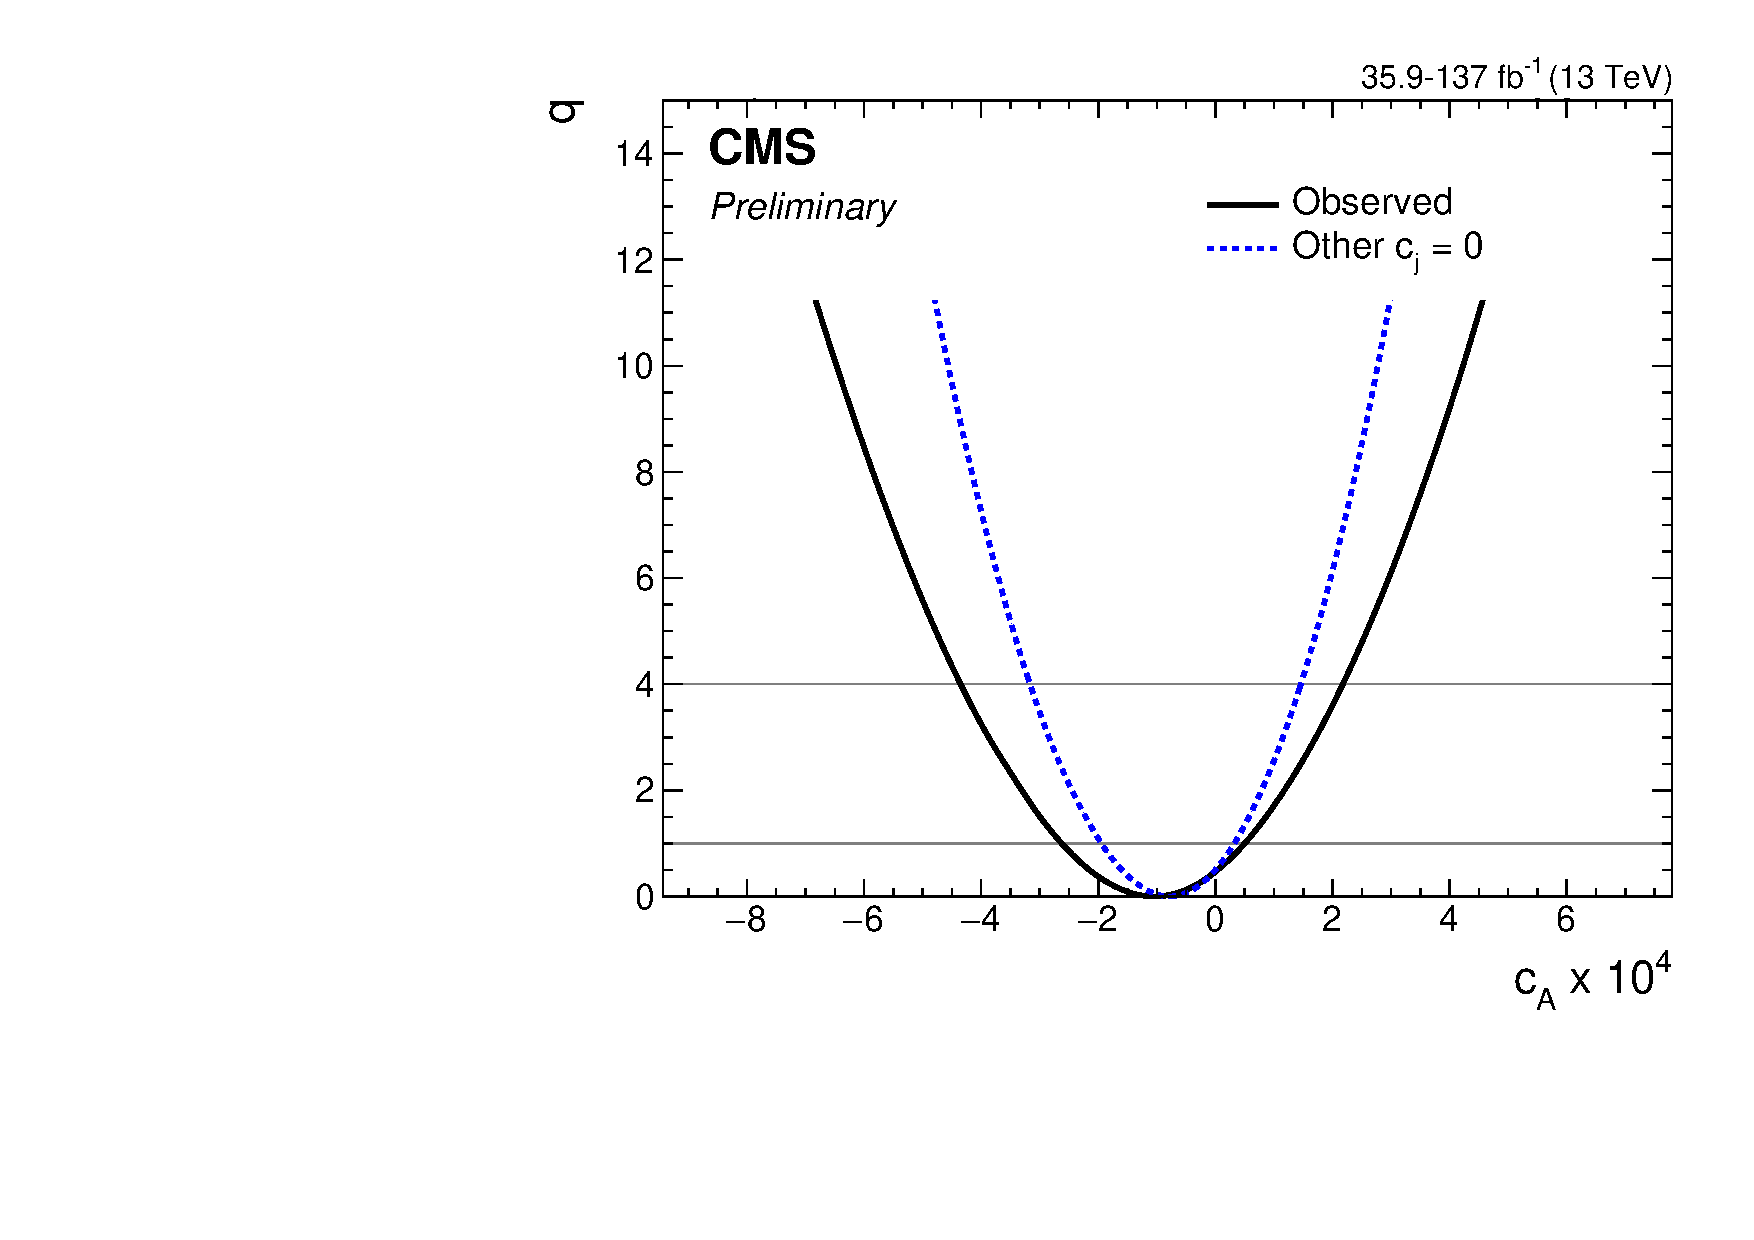
\includegraphics[width=.42\linewidth]{Figures/eft/cA_likelihood.pdf}
  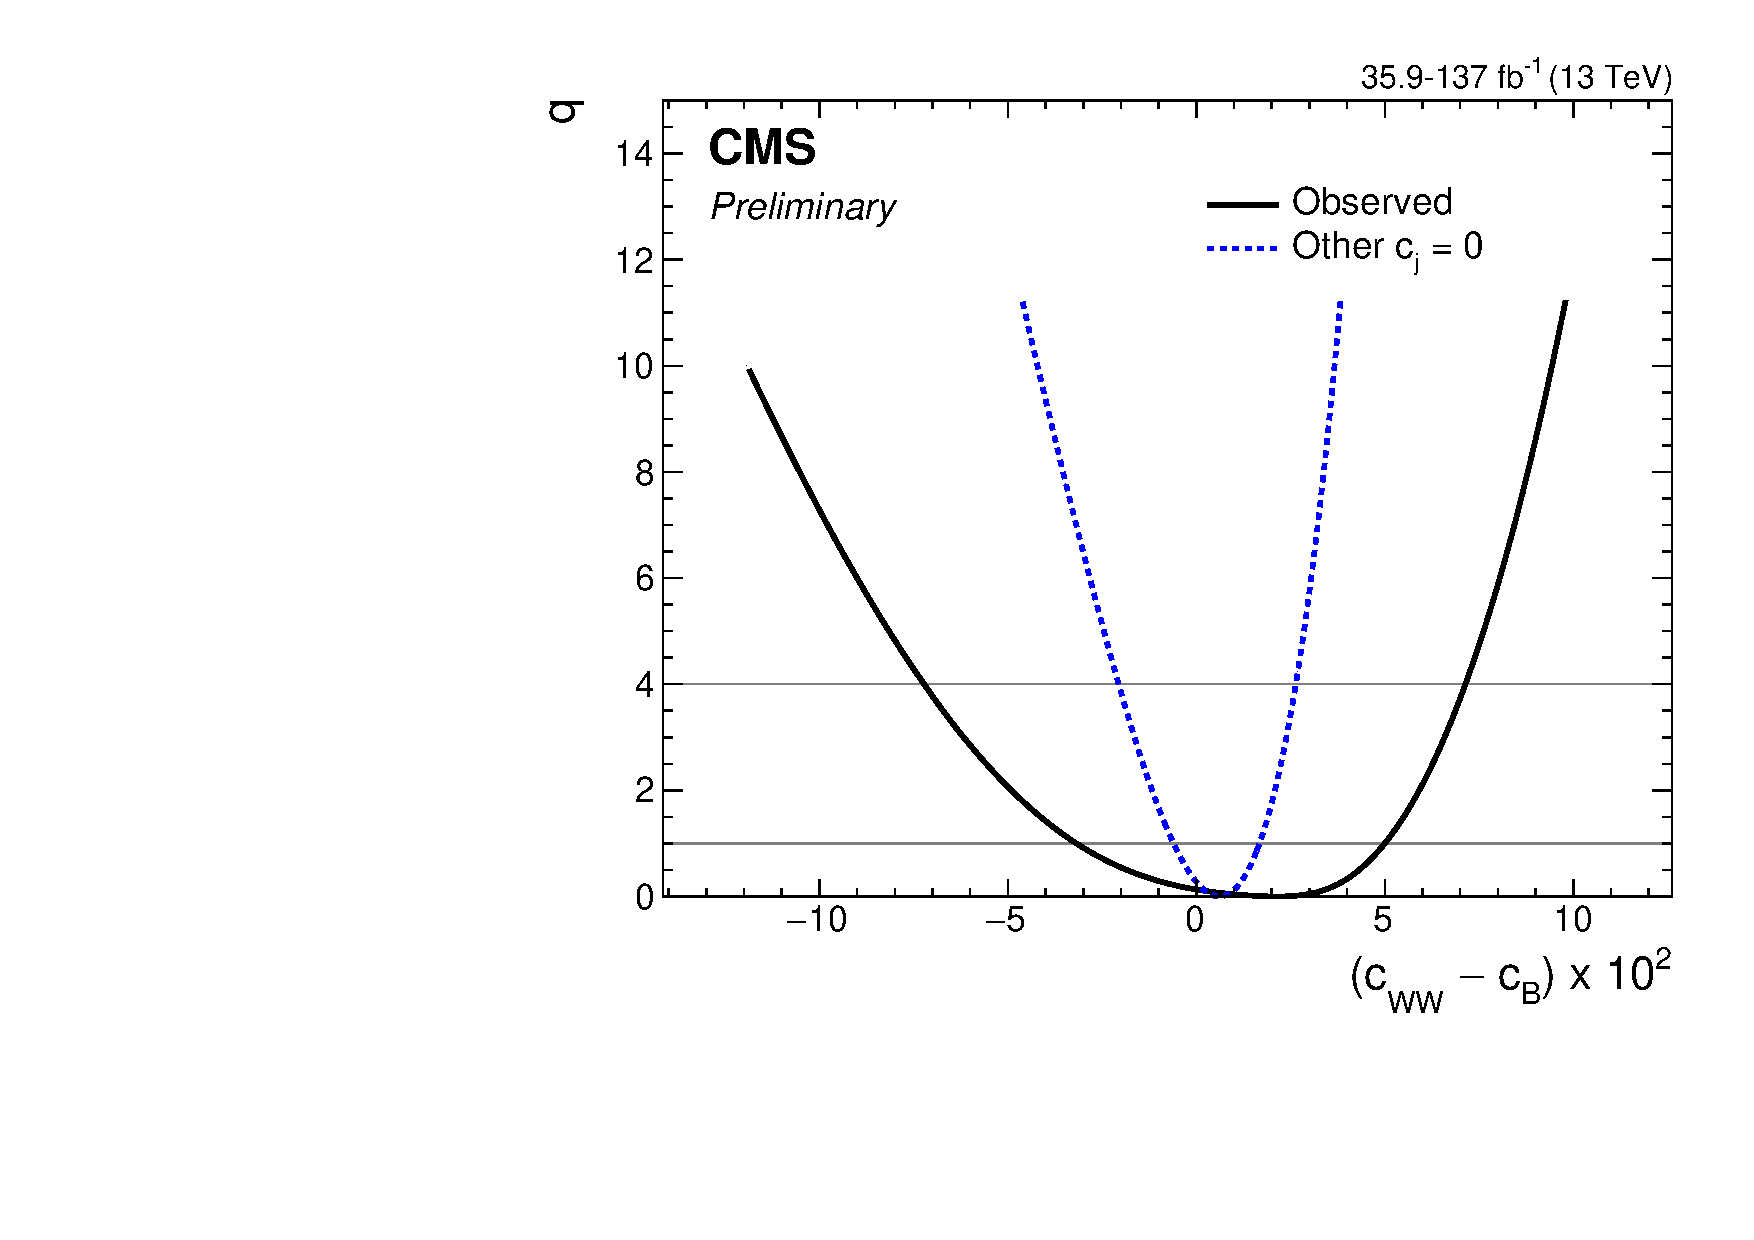
\includegraphics[width=.42\linewidth]{Figures/eft/cWWMinuscB_likelihood.pdf}
  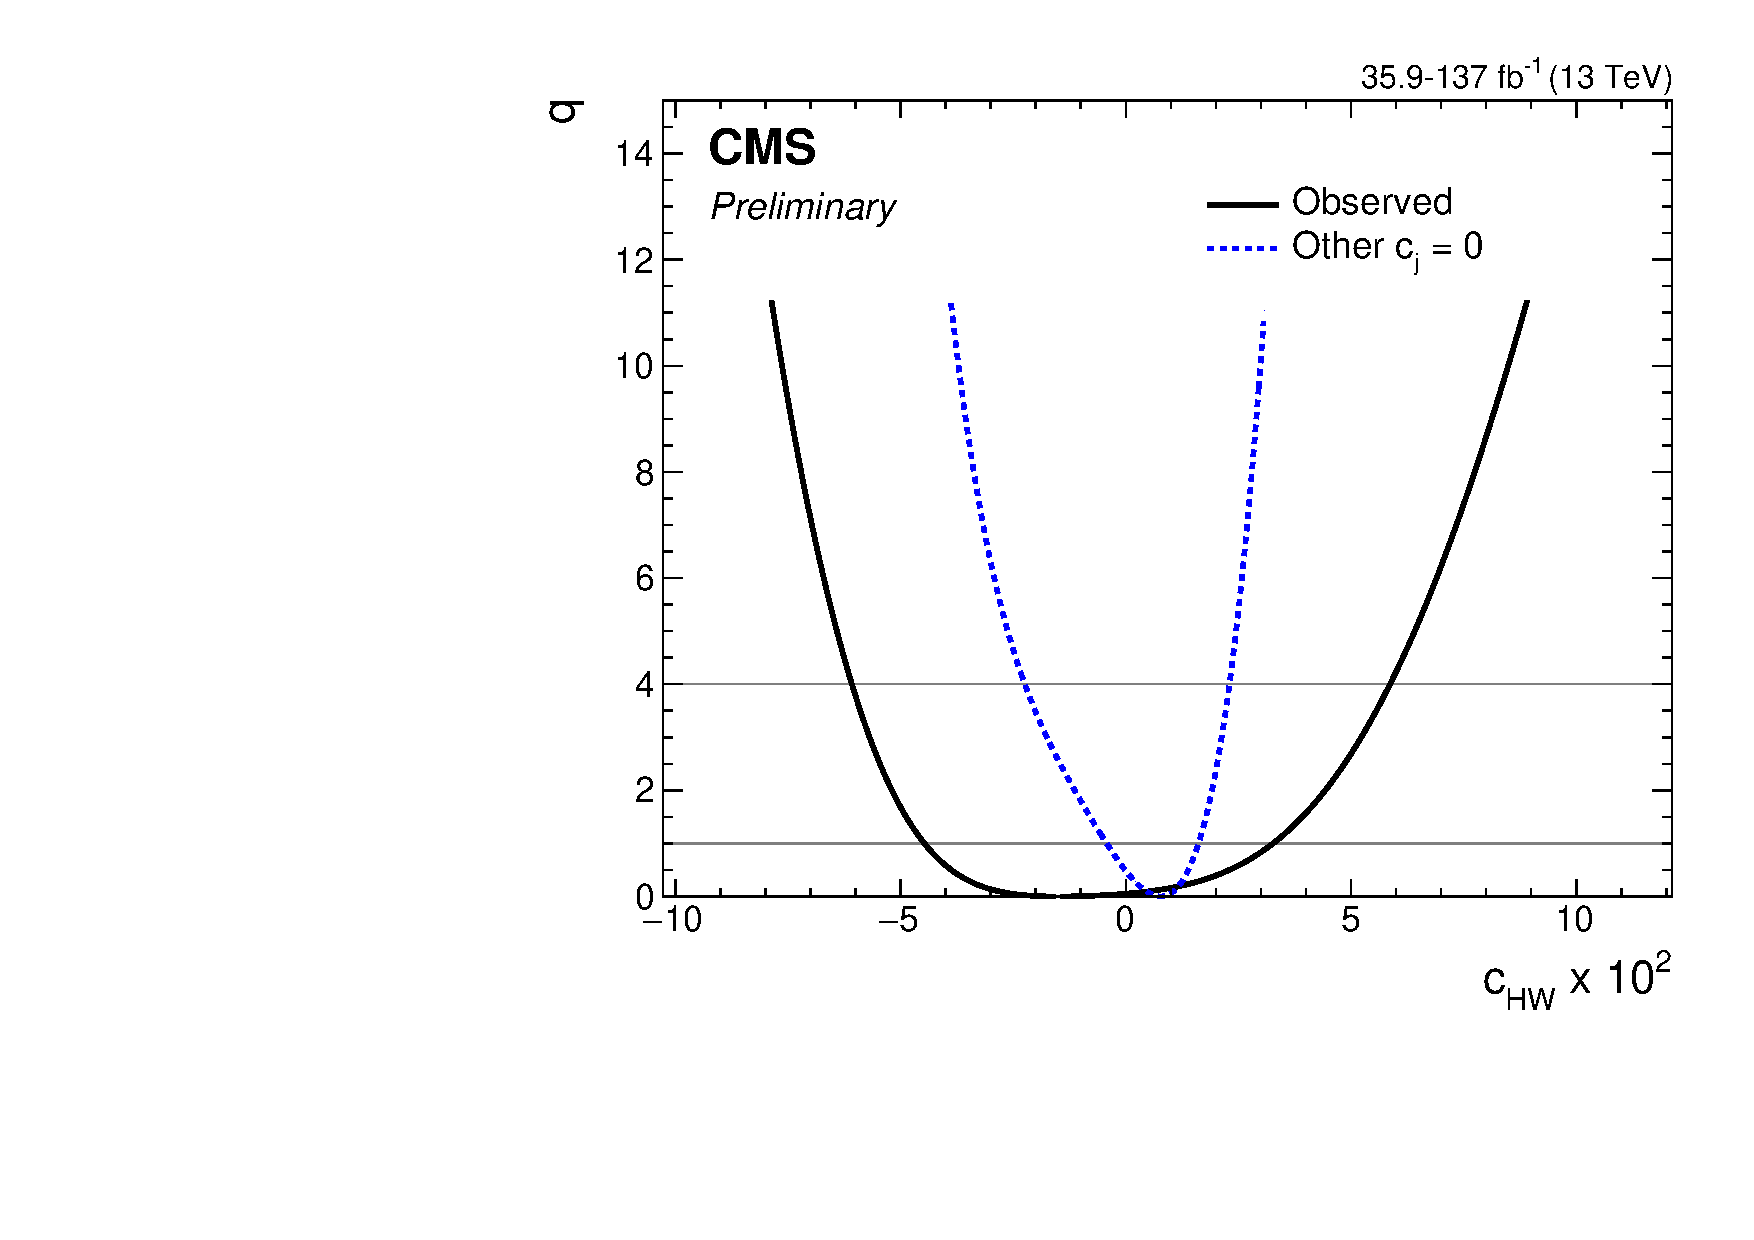
\includegraphics[width=.42\linewidth]{Figures/eft/cHW_likelihood.pdf}
  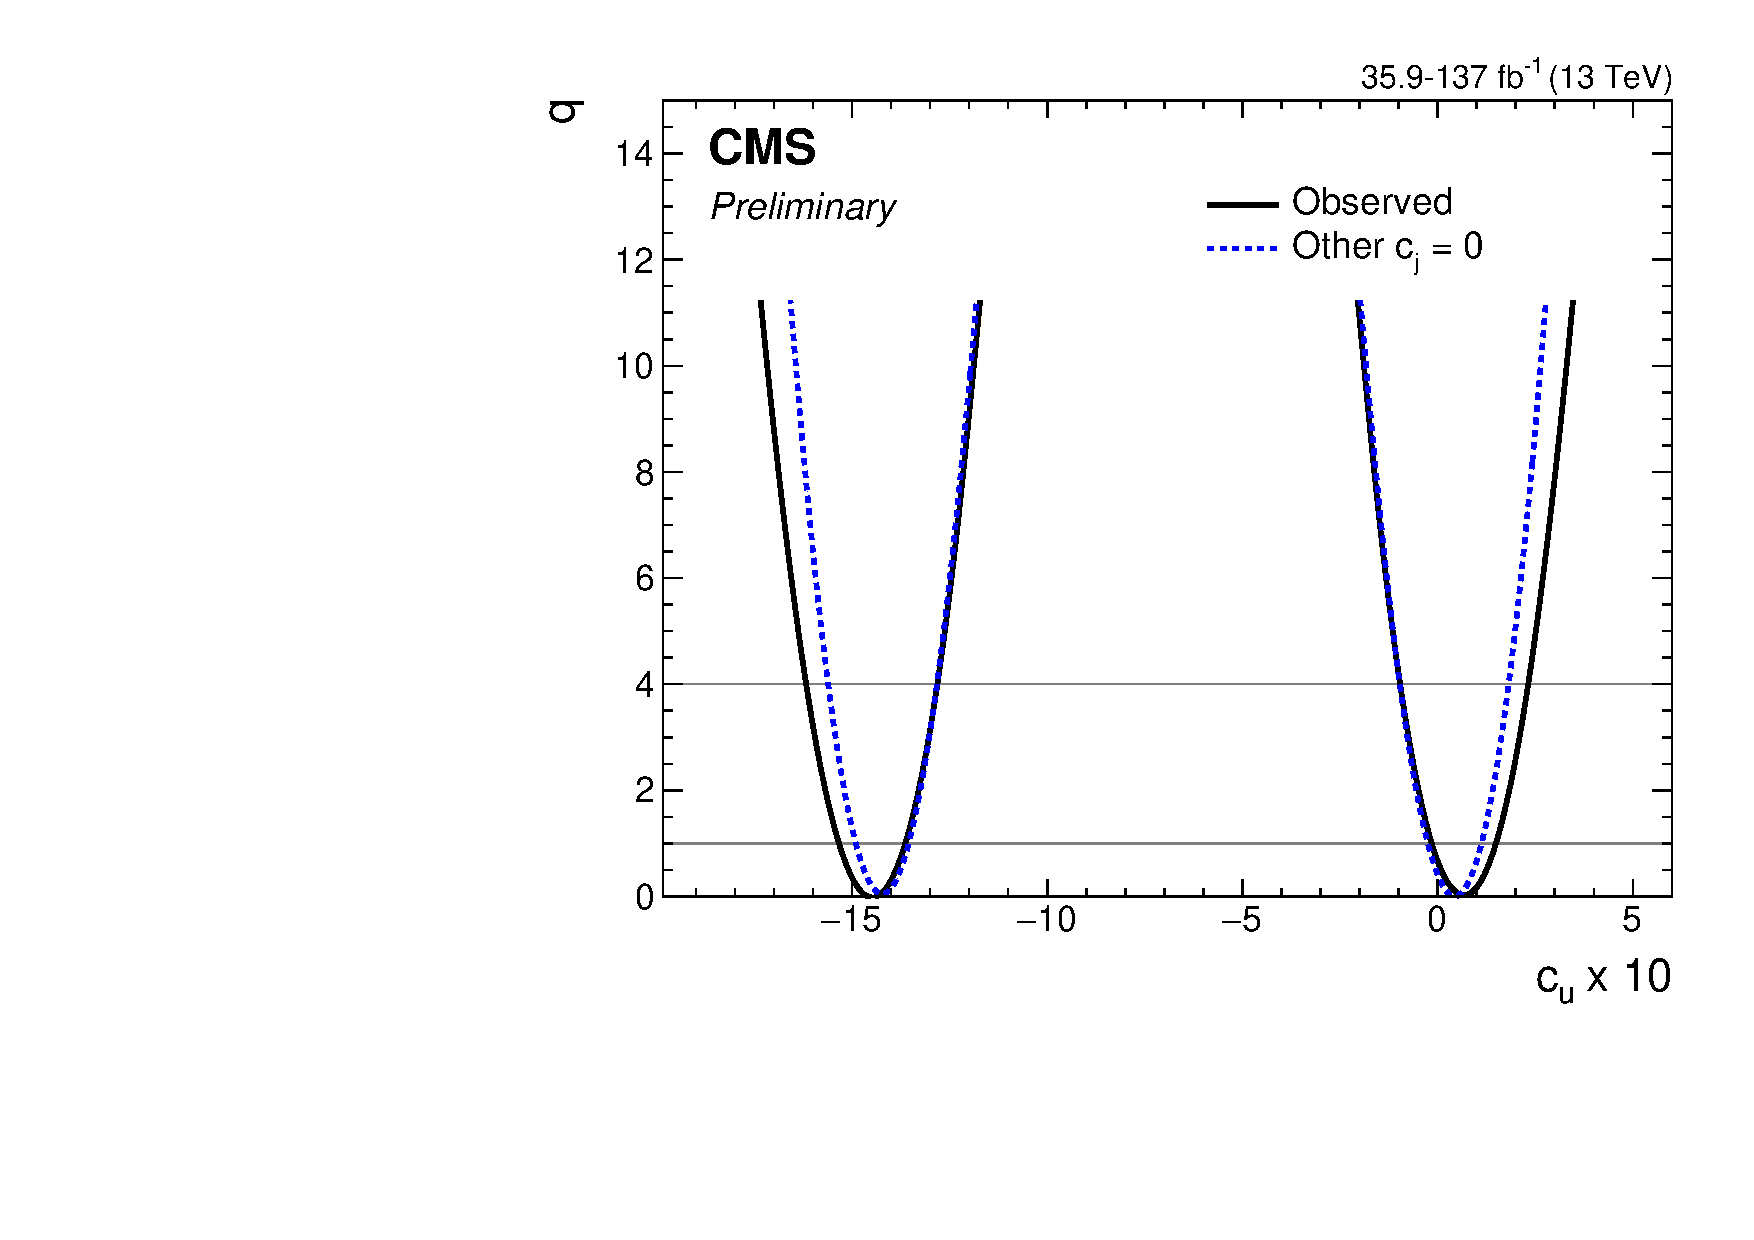
\includegraphics[width=.42\linewidth]{Figures/eft/cu_likelihood.pdf}
  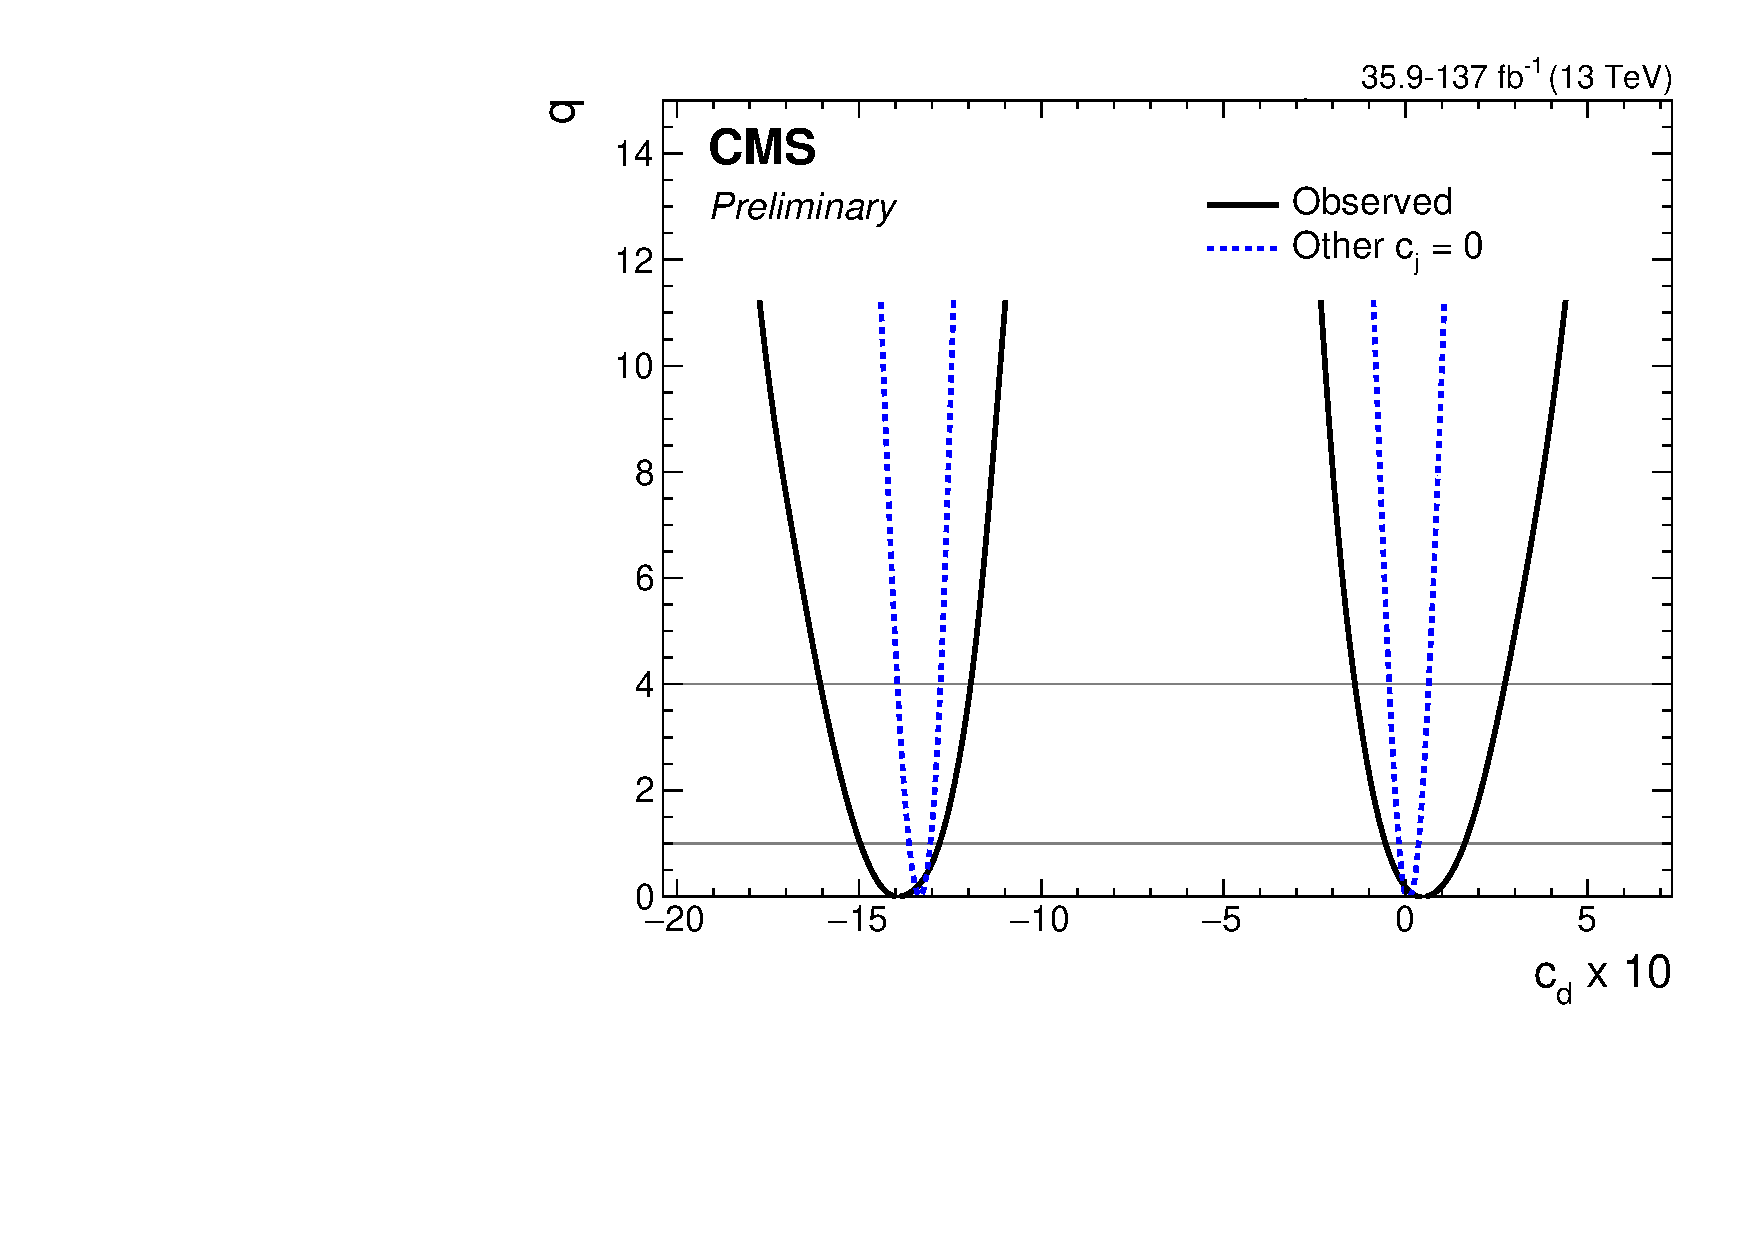
\includegraphics[width=.42\linewidth]{Figures/eft/cd_likelihood.pdf}
  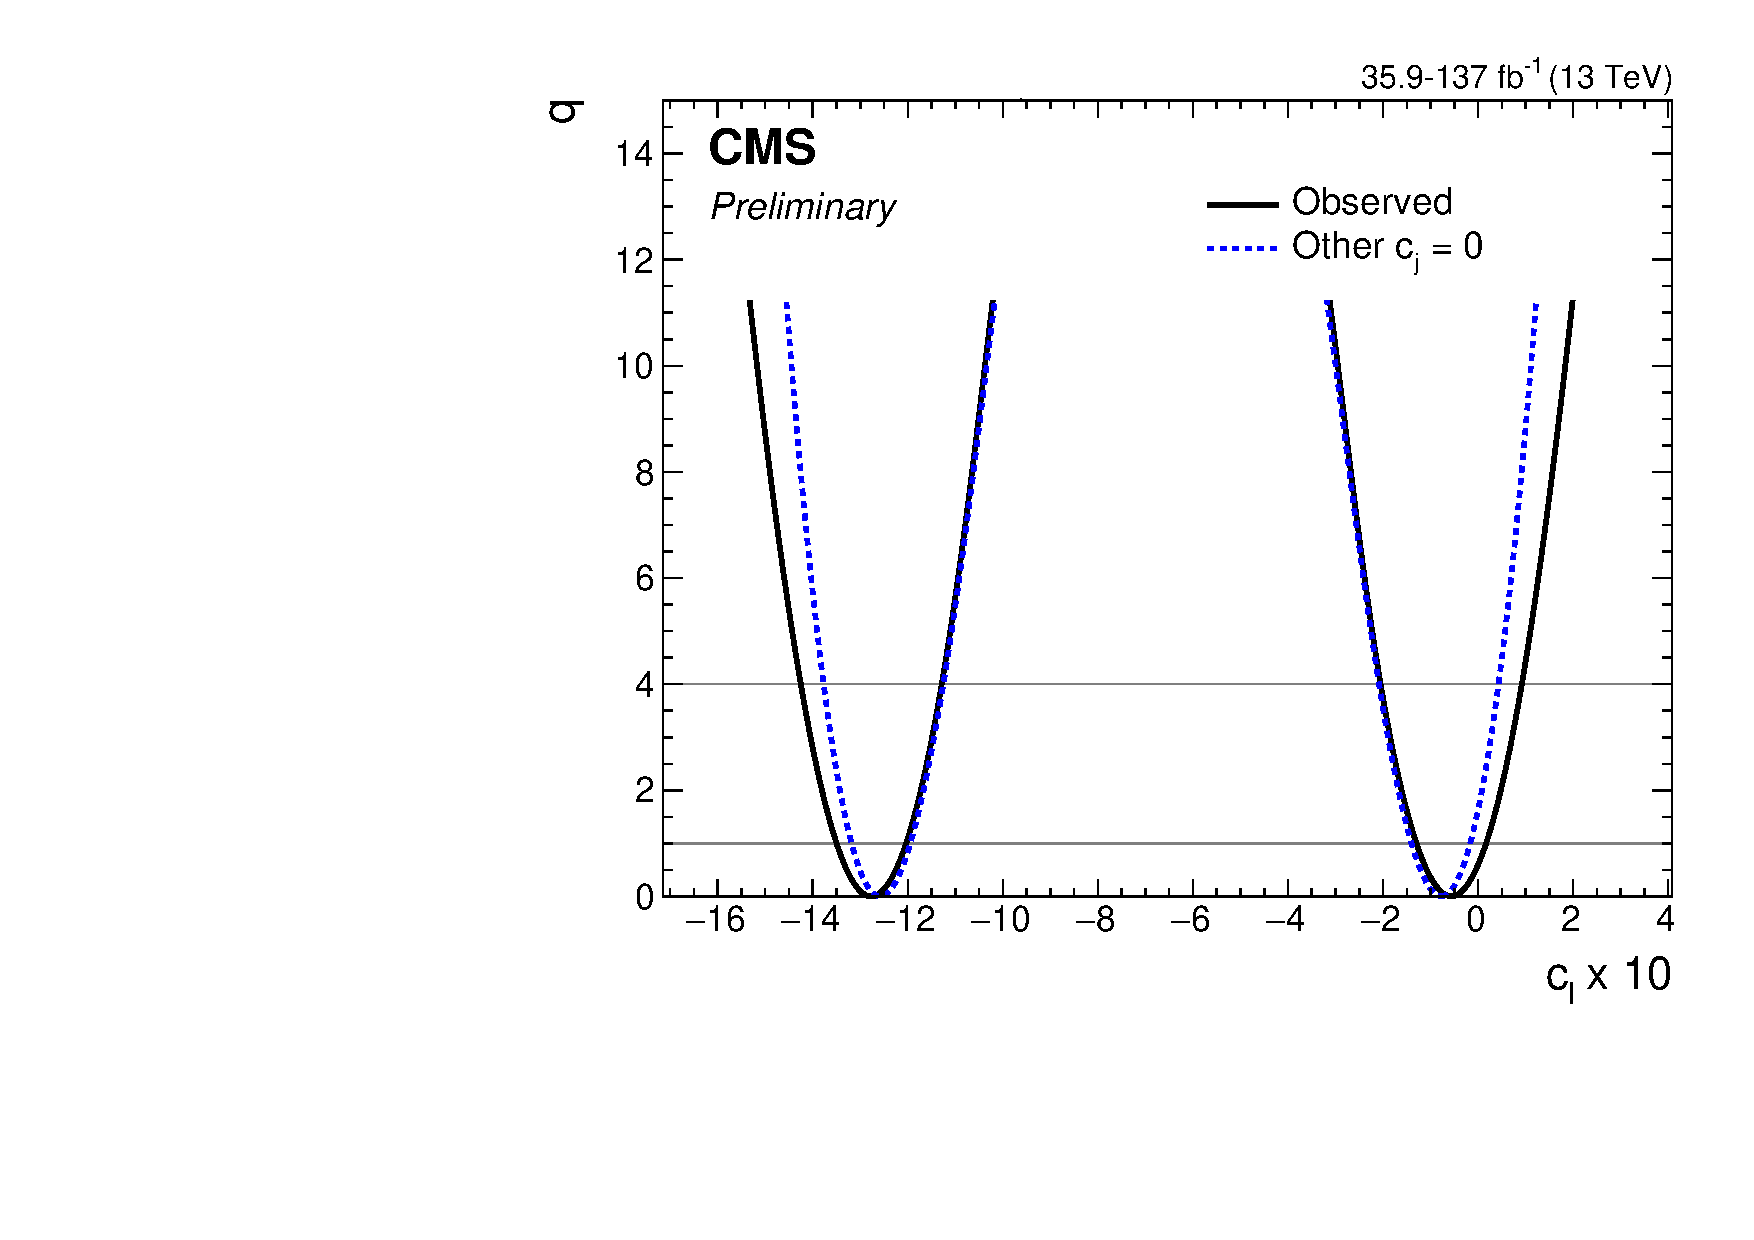
\includegraphics[width=.42\linewidth]{Figures/eft/cl_likelihood.pdf}
  \caption[Likelihood scans of the HEL parameters]
  {
    Plots of the $q(c_p)$ curves extracted in the HEL interpretation. The solid black (dashed blue) lines correspond to the fits in which the other HEL parameters are profiled (fixed to the SM). The horizontal lines at $q(c_p)$~=~1 and 4 indicate the 68\% and 95\% confidence intervals in $c_p$.
  }
  \label{fig:hel_likelihood_scans}
\end{figure}

The best-fit values of the HEL parameters, and the corresponding confidence intervals are summarised in Figures~\ref{fig:hel_results} and Table~\ref{tab:hel_results}. The double-minimum in the $c_u$, $c_d$, and $c_\ell$ likelihood scans originates from the degeneracy in the relevant scaling functions, where two points in the parameter space correspond to the SM prediction. For example, the $c_d$ constraint is driven by the measurement of the \Hbb branching fraction, which has a scaling function equal to unity for $c_d=0$ and $c_d=-4/3$. Including EFT variations in bbH production would help alleviate this degeneracy due to the introduction of a term $\propto c_d\,c_G$ in the bbH scaling function. Nevertheless, as described above, the bbH production mode is constrained to the SM prediction within theory uncertainties, since there is no dedicated analysis category targeting this production mode. 

\begin{figure}[htb!]
  \centering
  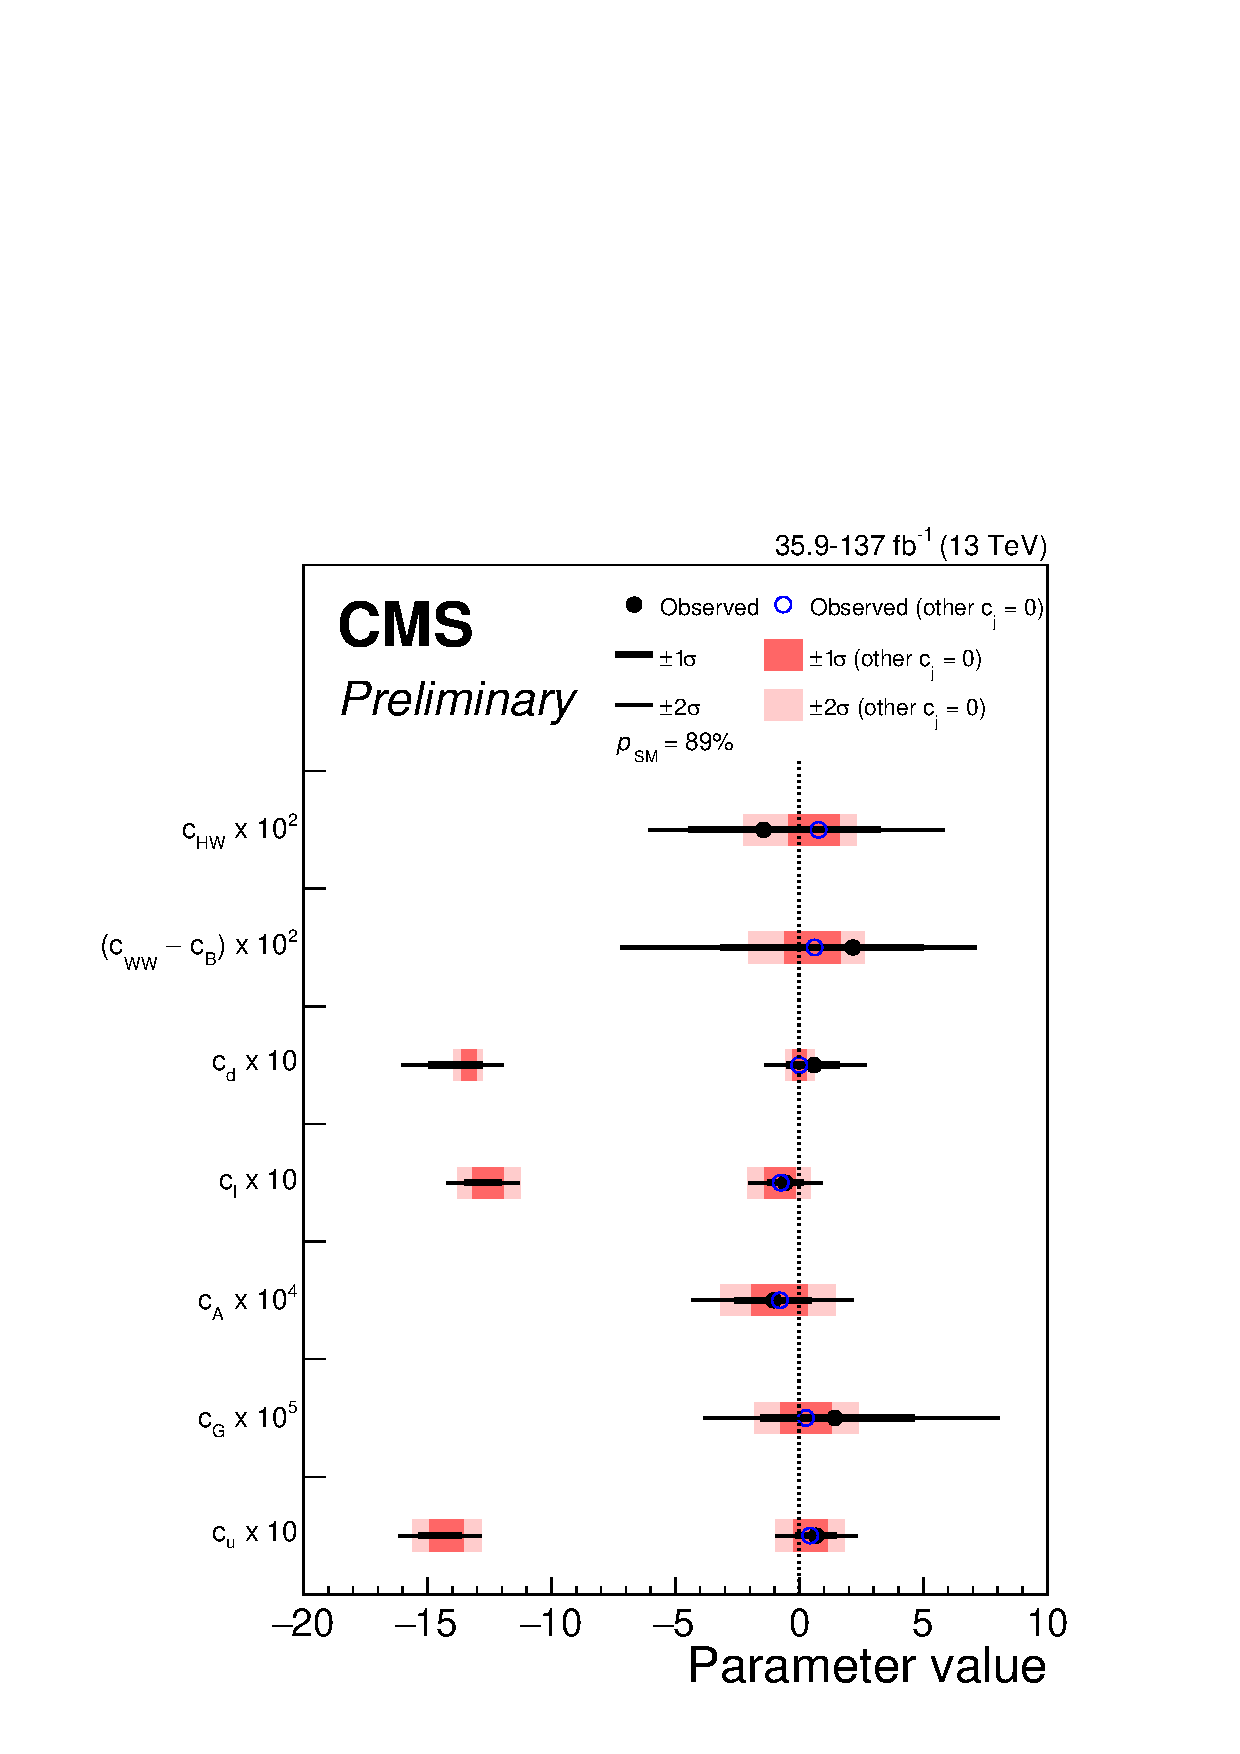
\includegraphics[width=.6\textwidth]{Figures/eft/hel_summary.pdf}
  \caption[Results of the HEL interpretation]
  {
    Observed best-fit values and confidence intervals for the parameters of interest in the HEL interpretation. The black circles, black thick lines, and black thin lines correspond to the best-fit values, the $\pm 1\sigma$ (68\%) confidence intervals, and the $\pm 2\sigma$ (95\%) confidence intervals, respectively, taken from the fits in which the other HEL parameters are profiled. The corresponding results from the fits in which the other HEL parameters are fixed to zero are shown by the hollow blue circles, the dark red bands and the light red bands respectively. The compatibility of the profiled fit with respect to the SM prediction is approximately $p_{\rm{SM}}=89\%$. 
  }
  \label{fig:hel_results}
\end{figure}

\begin{table}[htb]
  \centering
  \footnotesize
  \renewcommand{\arraystretch}{2.5}
  \setlength{\tabcolsep}{15pt}
  \caption[Results of the HEL interpretation]
  {
    The best-fit values with 68\% confidence intervals for the parameters of interest in the HEL interpretation. The results from both fitting scenarios are listed: profiling the other HEL parameters in the minimisation, and fixing the other HEL parameters to zero. The expected confidence intervals derived using the asimov data set are given in brackets. For the $c_u$, $c_d$ and $c_\ell$ parameters, the best-fit values and confidence intervals are stated for the minimum closest to zero in the respective $q(c_p)$ curves.
  }
  \label{tab:hel_results}
  \begin{tabular}{lcc}
  \multicolumn{3}{c}{\textbf{HEL interpretation}} \\ \hline 
  $\quad$Parameter & Others profiled & Fix others to SM \\ \hline
  
  \begin{tabular}{l}$c_G \times 10^5$\end{tabular} & \begin{tabular}{r@{}l@{}l}$1.43$ & {}$^{+3.20}_{-3.00}$ & $\Big($$^{+3.13}_{-2.74}$$\Big)$ \end{tabular} & \begin{tabular}{r@{}l@{}l}$0.27$ & {}$^{+1.05}_{-1.05}$ & $\Big($$^{+1.03}_{-1.01}$$\Big)$ \end{tabular} \\ 
  
  \begin{tabular}{l}$c_A \times 10^4$\end{tabular} & \begin{tabular}{r@{}l@{}l}$1.03$ & {}$^{+1.53}_{-1.59}$ & $\Big($$^{+1.59}_{-1.56}$$\Big)$ \end{tabular} & \begin{tabular}{r@{}l@{}l}$-0.78$ & {}$^{+1.11}_{-1.16}$ & $\Big($$^{+1.10}_{-1.11}$$\Big)$ \end{tabular} \\
  
  \begin{tabular}{l}$(c_{WW}-c_B) \times 10^2$\end{tabular} & \begin{tabular}{r@{}l@{}l}$2.16$ & {}$^{+2.84}_{-5.35}$ & $\Big($$^{+3.46}_{-5.00}$$\Big)$ \end{tabular} & \begin{tabular}{r@{}l@{}l}$0.62$ & {}$^{+1.06}_{-1.22}$ & $\Big($$^{+1.09}_{-1.23}$$\Big)$ \end{tabular} \\

  \begin{tabular}{l}$c_{HW} \times 10^2$\end{tabular} & \begin{tabular}{r@{}l@{}l}$-1.45$ & {}$^{+4.72}_{-3.03}$ & $\Big($$^{+3.93}_{-3.27}$$\Big)$ \end{tabular} & \begin{tabular}{r@{}l@{}l}$0.77$ & {}$^{+0.84}_{-1.20}$ & $\Big($$^{+1.04}_{-1.38}$$\Big)$ \end{tabular} \\
  
  \begin{tabular}{l}$c_u \times 10$\end{tabular} & \begin{tabular}{r@{}l@{}l}$0.68$ & {}$^{+0.82}_{-0.83}$ & $\Big($$^{+0.83}_{-0.79}$$\Big)$ \end{tabular} & \begin{tabular}{r@{}l@{}l}$0.43$ & {}$^{+0.69}_{-0.69}$ & $\Big($$^{+0.68}_{-0.67}$$\Big)$ \end{tabular} \\
  
  \begin{tabular}{l}$c_d \times 10$\end{tabular} & \begin{tabular}{r@{}l@{}l}$0.59$ & {}$^{+1.03}_{-1.13}$ & $\Big($$^{+1.08}_{-1.05}$$\Big)$ \end{tabular} & \begin{tabular}{r@{}l@{}l}$-0.01$ & {}$^{+0.31}_{-0.28}$ & $\Big($$^{+0.30}_{-0.28}$$\Big)$ \end{tabular} \\
  
  \begin{tabular}{l}$c_\ell \times 10$\end{tabular} & \begin{tabular}{r@{}l@{}l}$-0.57$ & {}$^{+0.74}_{-0.73}$ & $\Big($$^{+0.72}_{-0.77}$$\Big)$ \end{tabular} & \begin{tabular}{r@{}l@{}l}$-0.75$ & {}$^{+0.60}_{-0.64}$ & $\Big($$^{+0.58}_{-0.60}$$\Big)$ \end{tabular} \\
\end{tabular}
\end{table}

It is observed that both the best-fit values and confidence intervals can vary dramatically between the two fitting scenarios. This is especially true for the parameters which have sizeable correlations e.g. $c_{WW}-c_B$ and $c_{HW}$, and also for $c_d$ due to its large impact on the Higgs boson total width. The differences arise since the values of the other HEL parameters in the profiled fit can counter the impact from varying the parameter of interest, thus leading to a wider $q(c_p)$ curve. In contrast, this is not possible in the fit in which the other parameters are fixed to 0, resulting in narrower curves and therefore tighter constraints. This effect is less pronounced for the parameters which have smaller correlations and smaller effects on $\Gamma^H$: $c_u$, $c_A$ and $c_\ell$. 

The correlation coefficients between the HEL parameters are displayed in Figure \ref{fig:hel_correlations}. As mentioned above, a large correlation is observed between the pair of HEL parameters which mostly affect the HWW and HZZ vertices, namely $c_{HW}$ and $c_{WW}-c_B$. Including more granular measurements of the VH lep and qqH STXS bins will help reduce these correlations, since the $c_{HW}$ and $c_{WW}-c_B$ dependence varies for different kinematic regions of phase space. Moreover, large correlations are observed between $c_G$ and several other parameters. This results from the fact that the parametrisation is defined at LO. As a result the ggH production mode depends solely on $c_G$, and this dependence is relatively flat across all STXS bins. The $c_G$ parameter is therefore constrained by the total ggH production rate, which cannot be easily distinguished from an overall increase in the total Higgs boson decay width. The exceptions are $c_A$ and $c_l$, which show a small correlation with $c_G$ as they do not contribute significantly towards $\Gamma^H$. This property also explains the sizeable difference between the fixed and profiled $q(c_G)$ curves in Figure~\ref{fig:hel_likelihood_scans}.

\begin{figure}[htbp]
  \centering
  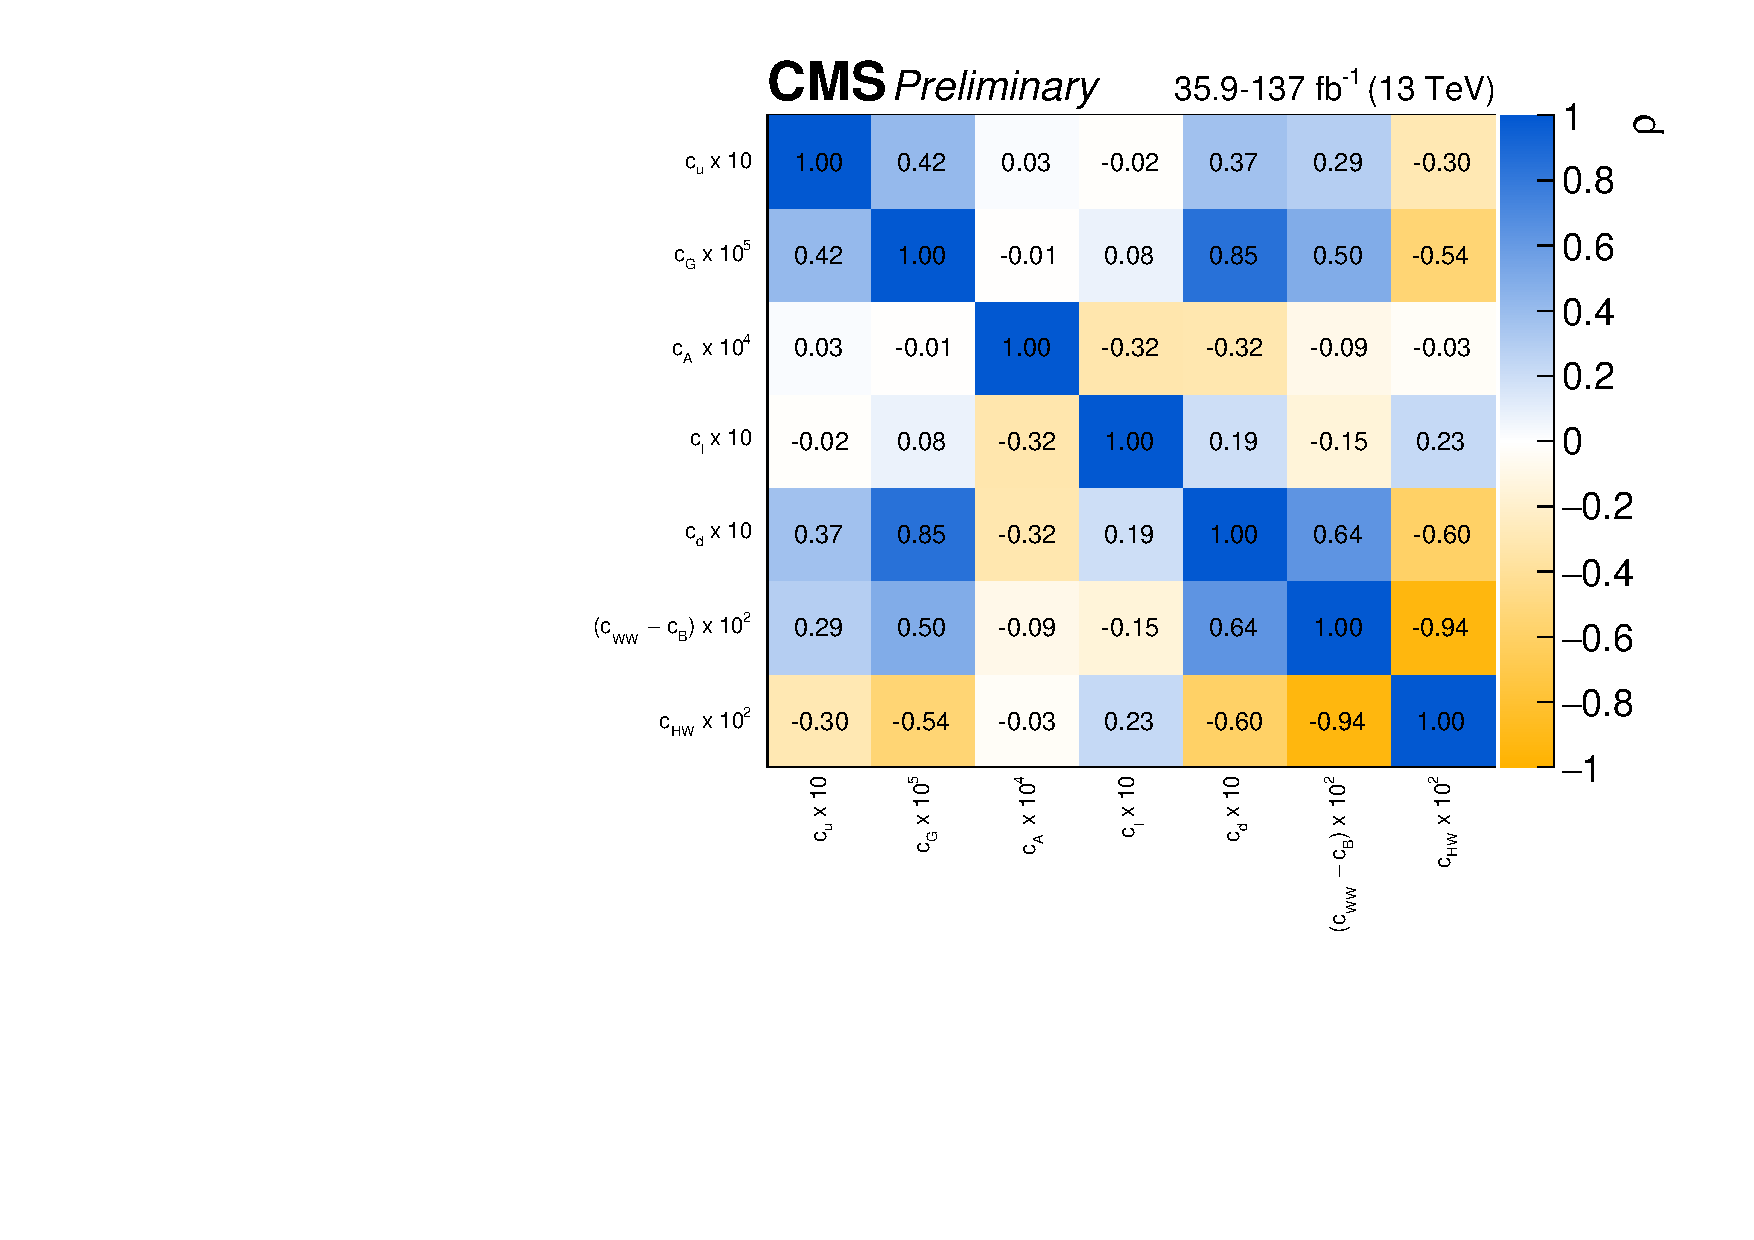
\includegraphics[width=.8\textwidth]{Figures/eft/hel_correlations.pdf}
  \caption[Correlations in HEL parameters]
  {
    Observed correlations between the parameters of interest in the HEL interpretation. The size of the correlations is indicated by the colour scale.
  }
  \label{fig:hel_correlations}
\end{figure}

All in all, the results are extremely compatible with the SM prediction. This is clearly visible in the $q(c_p)$ curves, such that all parameters in the profiled fit are in agreement with the SM prediction ($c_p=0$) within the 68\% confidence intervals. The corresponding $p$-value from the profiled fit, with respect to the SM hypothesis, is $p_{\rm{SM}}=89\%$. 

The uncertainties in the HEL parameters are amongst the most powerful constraints from Higgs boson measurements, thereby reducing the possible phase space for BSM physics in the Higgs sector. Naively, one can convert the constraints on the dimensionless HEL parameters, to a lower limit on the energy scale of new physics, $\Lambda$, by inverting the relationships defined in Table~\ref{tab:hel_operators}. \textbf{Is this reasoning valid?}. For example, the constraint on $c_G$,

\begin{equation}
    |c_G| \; \lesssim \; 5 \times 10^{-5} \; {\rm{@}} \; 68\% \; {\rm{C.L.}},
\end{equation}

\noindent
roughly corresponds to the following bound on the scale of new physics in the effective Hgg interaction vertex, assuming the nominal Wilson coefficient, $w_G$, is of order one,

\begin{equation}
    \Lambda^2 = \frac{m_W^2}{g_s^2}\Big| \frac{w_G}{c_G} \Big| \qquad \Rightarrow \qquad \Lambda \; \gtrsim \; 11~{\rm{TeV}} \; {\rm{@}} \; 68\% \; {\rm{C.L.}}\,.
\end{equation}

\noindent
Ultimately, the HEL model can be matched to UV-complete BSM theories. In doing so, the constraints in the HEL parameters shown here can be re-interpreted as constraints on the BSM couplings and masses of a UV-complete theory. A number of EFT matching examples are provided in Ref.~\cite{Marzocca:2020jze}. 

\subsection{Comparison to ATLAS result}
Table~\ref{tab:hel_atlas} compares the expected constraints\footnote{The expected constraints offer the best point of comparison in terms of the sensitivity, as they are not affected by statistical fluctuations in data.} extracted in this analysis to those from a previous result by the ATLAS collaboration~\cite{ATL-PHYS-PUB-2017-018}, which combined measurements from the \Hgg and \Hfl decay channels using 2016 data only (36.1~\fbinv). The improvements with respect to the ATLAS results are explained below for the common parameters of interest. It is important to keep in mind that this is not a perfect comparison since the ATLAS result considers a different HEL operator subset, $\{\mathcal{O}'\}$.

\begin{table}[htb]
  \centering
    %   \footnotesize
  \renewcommand{\arraystretch}{1.3}
  \setlength{\tabcolsep}{15pt}
  \caption[Comparison to the HEL parameter constraints from a previous ATLAS result]
  {
    The expected 68\% confidence intervals for the HEL parameters in the profiled fit. The equivalent constraints are shown from the ATLAS result documented in Ref.~\cite{ATL-PHYS-PUB-2017-018}. The final three rows show parameters which are not included in both the CMS and ATLAS operator subsets.
  }
  \label{tab:hel_atlas}
  \begin{tabular}{lcc}
\hline
  Parameter & ATLAS result~\cite{ATL-PHYS-PUB-2017-018} & CMS result \\ \hline
  $c_G \times 10^5$ & {}$^{+3.8}_{-2.6}$  & {}$^{+3.1}_{-2.7}$ \\ 
  
  $c_A \times 10^4$ & {}$^{+2.8}_{-2.2}$  & {}$^{+1.6}_{-1.6}$ \\
  
  $(c_{WW}-c_B) \times 10^2$ & {}$^{+5.7}_{-7.4}$  & {}$^{+3.4}_{-5.0}$ \\
  
  $c_{HW} \times 10^2$ & {}$^{+4.1}_{-4.3}$  & {}$^{+3.9}_{-3.3}$ \\

  $c_u \times 10$ & {}$^{+2.4}_{-2.8}$  & {}$^{+0.83}_{-0.79}$ \\ \hline
  
  $c_d \times 10$ & -  & {}$^{+1.1}_{-1.1}$ \\
  
  $c_\ell \times 10$ & -  & {}$^{+0.7}_{-0.8}$ \\ \hline
  
  $c_{HB} \times 10^1$ & {}$^{+1.4}_{-1.6}$  & - \\
  \hline

\end{tabular}
\end{table}

\begin{itemize}
    \item The constraint on $c_A$ improves by approximately 40\% due to the inclusion of the 2017 data (41.5~\fbinv) in the \Hgg channel. The improvement from the increased luminosity is not as large for $c_G$ since the constraint comes predominantly from ggH production which is limited by systematic uncertainties. Hence, there is a smaller gain from the increase in statistics.
    \item The constraint on $c_u$ improves dramatically ($\sim$70\%) due to the inclusion of analyses which specifically target ttH production in the CMS combination. 
    \item The inclusion of the \HWW and VH, \Hbb measurements in the combination, in addition to the increased statistics in the \Hfl channel, leads to an improvement in the constraint on $c_{WW}-c_B$ by approximately 35\%. Nevertheless, the improvement is somewhat hampered by the differences between the CMS and HXSWG parametrisation, described in section \ref{sec:hel_validation}. For $c_{HW}$, the parametrisation differences have a larger effect, resulting in a smaller improvement in the constraint ($\sim$15\%).
    \item The $c_d$ and $c_\ell$ parameters were not considered in Ref~\cite{ATL-PHYS-PUB-2017-018}, since their constraints are driven mainly from the \Hbb and \Htautau channels. The $c_{HB}$ parameter is not considered in the CMS interpretation.
\end{itemize}

Recently, the ATLAS collaboration have superseded the result of Ref.~\cite{ATL-PHYS-PUB-2017-018} with an EFT interpretation of STXS measurements in the \Hbb, \Hgg and \Hfl decay channels, using data taken during the 2016-2018 periods~\cite{ATLAS-CONF-2020-053}. This corresponds to a total integrated luminosity of 139~\fbinv in each of the input channels. The interpretation is performed in the Warsaw basis~\cite{Grzadkowski:2010es} (see section \ref{sec:smeftsim}), where the \texttt{SMEFTsim} model~\cite{Brivio:2017btx} is utilised to derive the EFT parametrisation. Due to the difference in EFT bases, it is difficult to make a direct comparison with the results of the HEL interpretation shown here. The next CMS Higgs boson combination will include an EFT interpretation in the Warsaw basis, based on the combination of STXS stage 1.2 measurements in all of the major Higgs boson decay channels. More detail regarding this future CMS analysis is provided in section \ref{sec:smeftsim}.

\subsection{Comparison to the simplified re-interpretation procedure}
The differences between the $q(c_p)$ curves in Figure~\ref{fig:hel_likelihood_scans} and the $\Delta\chi^2(c_p)$ curves in Figures~\ref{fig:hel_chi2_simplified_0}--\ref{fig:hel_chi2_simplified_1} directly reflect the assumptions of the simplified re-interpretation procedure. Namely, assuming the likelihood surface is Gaussian and therefore the measurement uncertainties are symmetric, and also treating the input analyses as statistically independent. The results from both approaches are summarised in Table~\ref{tab:hel_simplified_comp}.

\begin{table}[htb!]
  \centering
  \footnotesize
  \renewcommand{\arraystretch}{1.6}
  \setlength{\tabcolsep}{2pt}
  \caption[Comparison to the HEL parameter constraints from the simplified re-interpretation procedure]
  {
    The best-fit values and 68\% confidence intervals for the HEL parameters extracted using the full likelihood results extraction and the simplified re-interpretation procedure. The expected 68\% confidence intervals are given in brackets.
  }
  \label{tab:hel_simplified_comp}
  \begin{tabular}{l|rr|rr}
    \hline
  \multirow{2}{*}{$\quad$Parameter} & \multicolumn{2}{c|}{Other profiled} & \multicolumn{2}{c}{Fix others to SM} \\
  & \multicolumn{1}{c}{Full $q$} & \multicolumn{1}{c|}{$\Delta\chi^2$} & \multicolumn{1}{c}{Full $q$} & \multicolumn{1}{c}{$\Delta\chi^2$} \\ \hline
  
  \begin{tabular}{l}$c_G \times 10^5$\end{tabular} & 
  \begin{tabular}{r@{}l@{}l}$1.43$ & {}$^{+3.20}_{-3.00}$ & $\Big($$^{+3.13}_{-2.74}$$\Big)$ \end{tabular} & \begin{tabular}{r@{}l@{}l}$1.44$ & {}$^{+2.77}_{-2.31}$ & $\Big($$^{+2.92}_{-2.41}$$\Big)$ \end{tabular} &
  \begin{tabular}{r@{}l@{}l}$0.27$ & {}$^{+1.05}_{-1.05}$ & $\Big($$^{+1.03}_{-1.01}$$\Big)$ \end{tabular} &
  \begin{tabular}{r@{}l@{}l}$-0.27$ & {}$^{+0.82}_{-0.85}$ & $\Big($$^{+0.82}_{-0.85}$$\Big)$ \end{tabular} \\
  
  \begin{tabular}{l}$c_A \times 10^4$\end{tabular} & 
  \begin{tabular}{r@{}l@{}l}$-1.03$ & {}$^{+1.53}_{-1.59}$ & $\Big($$^{+1.59}_{-1.56}$$\Big)$ \end{tabular} &
  \begin{tabular}{r@{}l@{}l}$0.97$ & {}$^{+1.31}_{-1.60}$ & $\Big($$^{+1.49}_{-1.55}$$\Big)$ \end{tabular} &
  \begin{tabular}{r@{}l@{}l}$-0.78$ & {}$^{+1.11}_{-1.16}$ & $\Big($$^{+1.10}_{-1.11}$$\Big)$ \end{tabular} &
  \begin{tabular}{r@{}l@{}l}$1.08$ & {}$^{+1.01}_{-0.97}$ & $\Big($$^{+1.06}_{-1.01}$$\Big)$ \end{tabular} \\
  
  \begin{tabular}{l}$(c_{WW}-c_B) \times 10^2$\end{tabular} & 
  \begin{tabular}{r@{}l@{}l}$2.16$ & {}$^{+2.84}_{-5.35}$ & $\Big($$^{+3.46}_{-5.00}$$\Big)$ \end{tabular} &
  \begin{tabular}{r@{}l@{}l}$-0.11$ & {}$^{+2.49}_{-3.37}$ & $\Big($$^{+2.87}_{-3.76}$$\Big)$ \end{tabular} &
  \begin{tabular}{r@{}l@{}l}$0.62$ & {}$^{+1.06}_{-1.22}$ & $\Big($$^{+1.09}_{-1.23}$$\Big)$ \end{tabular} &
  \begin{tabular}{r@{}l@{}l}$0.25$ & {}$^{+0.91}_{-1.06}$ & $\Big($$^{+0.98}_{-1.16}$$\Big)$ \end{tabular} \\

  \begin{tabular}{l}$c_{HW} \times 10^2$\end{tabular} & 
  \begin{tabular}{r@{}l@{}l}$-1.45$ & {}$^{+4.72}_{-3.03}$ & $\Big($$^{+3.93}_{-3.27}$$\Big)$ \end{tabular} &
  \begin{tabular}{r@{}l@{}l}$0.54$ & {}$^{+2.19}_{-2.24}$ & $\Big($$^{+2.71}_{-2.67}$$\Big)$ \end{tabular} &
  \begin{tabular}{r@{}l@{}l}$0.77$ & {}$^{+0.84}_{-1.20}$ & $\Big($$^{+1.04}_{-1.38}$$\Big)$ \end{tabular} &
  \begin{tabular}{r@{}l@{}l}$0.55$ & {}$^{+0.60}_{-0.71}$ & $\Big($$^{+0.80}_{-1.09}$$\Big)$ \end{tabular} \\
  
  \begin{tabular}{l}$c_u \times 10$\end{tabular} & 
  \begin{tabular}{r@{}l@{}l}$0.68$ & {}$^{+0.82}_{-0.83}$ & $\Big($$^{+0.83}_{-0.79}$$\Big)$ \end{tabular} &
  \begin{tabular}{r@{}l@{}l}$0.64$ & {}$^{+0.68}_{-0.74}$ & $\Big($$^{+0.76}_{-0.76}$$\Big)$ \end{tabular} &
  \begin{tabular}{r@{}l@{}l}$0.43$ & {}$^{+0.69}_{-0.69}$ & $\Big($$^{+0.68}_{-0.67}$$\Big)$ \end{tabular} &
  \begin{tabular}{r@{}l@{}l}$0.50$ & {}$^{+0.57}_{-0.60}$ & $\Big($$^{+0.65}_{-0.70}$$\Big)$ \end{tabular} \\
  
  \begin{tabular}{l}$c_d \times 10$\end{tabular} & 
  \begin{tabular}{r@{}l@{}l}$0.59$ & {}$^{+1.03}_{-1.13}$ & $\Big($$^{+1.08}_{-1.05}$$\Big)$ \end{tabular} &
  \begin{tabular}{r@{}l@{}l}$0.52$ & {}$^{+1.02}_{-0.64}$ & $\Big($$^{+1.38}_{-0.81}$$\Big)$ \end{tabular} &
  \begin{tabular}{r@{}l@{}l}$-0.01$ & {}$^{+0.31}_{-0.28}$ & $\Big($$^{+0.30}_{-0.28}$$\Big)$ \end{tabular} &
  \begin{tabular}{r@{}l@{}l}$0.26$ & {}$^{+0.28}_{-0.26}$ & $\Big($$^{+0.26}_{-0.24}$$\Big)$ \end{tabular} \\
  
  \begin{tabular}{l}$c_\ell \times 10$\end{tabular} & 
  \begin{tabular}{r@{}l@{}l}$-0.57$ & {}$^{+0.74}_{-0.73}$ & $\Big($$^{+0.72}_{-0.77}$$\Big)$ \end{tabular} &
  \begin{tabular}{r@{}l@{}l}$-0.89$ & {}$^{+0.78}_{-0.77}$ & $\Big($$^{+0.73}_{-0.67}$$\Big)$ \end{tabular} &
  \begin{tabular}{r@{}l@{}l}$-0.75$ & {}$^{+0.60}_{-0.64}$ & $\Big($$^{+0.58}_{-0.60}$$\Big)$ \end{tabular} &
  \begin{tabular}{r@{}l@{}l}$-0.89$ & {}$^{+0.64}_{-0.71}$ & $\Big($$^{+0.57}_{-0.62}$$\Big)$ \end{tabular} \\
  \hline
\end{tabular}
\end{table}

In general, the two approaches are in decent agreement. This is particularly true for the expected sensitivities, given in brackets, and for (the majority of) the fits in which the other parameters are fixed to zero. For the profiled fits, the agreement is less good. This is because the profiled fit represents a more complicated problem, where certain nuances of the likelihood, such as the correlations between input measurements, become increasingly important. The complexity of the CMS Higgs boson combination likelihood makes it extremely difficult to pinpoint the origins of the differences. This ultimately motivates \textit{in-house} EFT interpretations, such as the one presented here, since the experiments have access to the full likelihood function.

It should be stressed that there exist more in-depth methods for performing re-interpretations. An extension to the simplified re-interpretation procedure used here is described in Ref.~\cite{Kraml:2019sis}, which introduces a variable Gaussian function to deal with asymmetric uncertainties. Experiments are also beginning to publish simplified or full likelihood functions to accompany their measurements, which can be used for future re-interpretation~\cite{10.21468SciPostPhys.9.2.022}. Furthermore, the use of ML algorithms to predict the likelihood function or even perform likelihood-free inference has been studied~\cite{Coccaro:2019lgs,Cranmer:2015bka,Brehmer:2020cvb}. These methods, which will systematically improve the accuracy of the re-interpretation, are not discussed any further in this thesis.

\section{The future of Higgs EFT measurements in CMS}\label{sec:eft_improving}
The interest in using SMEFT to parametrise the effects of many candidate BSM theories has increased substantially in recent years. The HEL interpretation discussed in this chapter was the first application of a SMEFT to STXS measurements at CMS. Going forward, the obvious means to tightening the constraints on the parameters of interest in this approach, is to use more data, thereby decreasing the statistical uncertainties. In addition, increasing the granularity of the measurements will help disentangle regions of phase space that depend differently on the EFT parameters. Not only does this result in tighter constraints and smaller correlations due to the kinematic information available in the measurements, but it also allows more directions (more operators) in the EFT to be probed.  

The CMS collaboration will perform a combination of Higgs boson measurements from all the major decay channels, using the full data set collected in the period 2016-2018\footnote{Including the \Hgg measurements described in chapters~\ref{chap:hgg_overview}--\ref{chap:hgg_results}.}. This corresponds to an integrated luminosity of 137~\fbinv in all input analyses. In the combination, the signal processes will be defined at the granularity of the STXS stage 1.2 binning scheme, thus enabling a highly granular EFT interpretation of STXS measurements, akin to the ATLAS result of Ref.~\cite{ATLAS-CONF-2020-053}. Of course, this will only be possible when all of the individual input analyses to the combination have been finalised.

The HEL interpretation discussed in this chapter provided a solid platform on which to build EFT interpretations of STXS measurements at CMS. Nevertheless, there are a number of caveats associated with the result. These include the choice of operator basis in the EFT expansion, the effect of higher order corrections in the parametrisation, the impact of neglecting acceptance effects, and the usefulness of STXS measurements as opposed to dedicated EFT analyses which are constructed to maximise the sensitivity to the EFT parameters. This section will discuss the implication of these caveats, and how they may be addressed in future Higgs EFT measurements at CMS.

\subsection{Warsaw basis: SMEFTsim}\label{sec:smeftsim}
The first item to be addressed is the choice of operator basis. Ultimately, the choice of basis only becomes relevant when the effect of certain operators are set to zero; new physics will appear equivalently in any complete operator expansion. However, given the limited available statistics and limited breadth of measurements, it is infeasible to constrain all EFT operators simultaneously. As a result, some operators must be fixed to zero, and the choice of basis becomes important.

The interpretation described in this chapter has been performed using a partial implementation of the SILH basis, known as the Higgs Effective Lagrangian~\cite{Alloul:2013naa}. Whilst the SILH basis benefits from being relatively straightforward to match to UV-complete models with modified bosonic interactions, and is easily propagated to the impact on LEP observables, it suffers from the fact that the same operators contribute to both anomalous triple gauge couplings (aTGC) in EW measurements and Higgs observables~\cite{Falkowski:2015wza}. Since performing this interpretation, the emphasis in the high energy physics community has shifted towards the \textit{Warsaw basis}~\cite{Grzadkowski:2010es}. The Warsaw basis is more appropriate for BSM physics with modified fermionic interactions, and has already been used in a number of Higgs, EW and top-quark measurements\footnote{Some examples are provided in Refs.~\cite{ATLAS-CONF-2020-053,,Sirunyan:2020tqm,Sirunyan:2020jtq}.}. By adopting a common language in the EFT interpretations, it becomes possible to combine results from multiple disciplines (Higgs, EW, top), thus enabling the ultimate consistency test of the SM in which many directions of the EFT parameter space can be probed simultaneously. Motivated by this notion of a cross-discipline \textit{global combination}, future EFT interpretations of STXS measurements at CMS will be performed in the Warsaw basis.

The \texttt{SMEFTsim} package~\cite{Brivio:2017btx} provides a number of LO implementations of the complete Warsaw basis, up to operators of dimension-6, with different assumptions regarding the flavour symmetry. The implementation discussed in the following section assumes a ${\rm{U}}(3)^5$ flavour symmetry i.e. unbroken global flavour symmetry present in the SM outside the Yukawa sector, and includes the possibility of CP-violating phases. The model is configured using the theoretically-favoured $m_W$, $m_Z$ and $G_F$ input parameter scheme. Additionally, the Warsaw basis parameters, $\vec{C}$ (capitalised to help differentiate from the HEL parameters, $\vec{c}$), are defined for a nominal energy scale of $\Lambda$~=~1~TeV. This differs from the HEL parameters, which absorbed the $\Lambda^{-2}$ factor into their definition. Nevertheless, the Warsaw basis parameters can be obtained for alternate values of $\Lambda$~=~$\Lambda^*$ by scaling with factor ($\Lambda^*$/1~TeV)$^2$.

\subsection{Warsaw parametrisation and expected sensitivities}
The signal yield parametrisation has been derived in the Warsaw basis using the same procedure detailed in section \ref{sec:hel_derivation}. All MC generator options are identical to those defined in Appendix~\ref{app:generator_options}, except the \texttt{HEL\_UFO} model has been exchanged with the \texttt{SMEFTsim} model. The parametrisation is defined at the granularity of the STXS stage 1.2 binning scheme to match the input analyses in the future CMS Higgs boson combination. 

Again, non-zero effects are considered in only a subset of EFT operators, since it is not possible to constrain all directions of parameter space using Higgs boson measurements alone. A larger number of operators, listed in Table~\ref{tab:smeft_operators}, are included in this parametrisation to account for the enhanced sensitivity from the increased integrated luminosity and more granular measurements. The full set of cross section and branching fraction scaling functions are derived in the Warsaw basis including both the linear and quadratic terms, and are tabulated in Appendix~\ref{app:smeft_parametrisation}. As an example, the scaling terms for the ZH lep and ttH stage 1.2 bins are shown as functions of the $C_{HW}$ and $|C_{uG}|$ Warsaw basis parameters, respectively, in Figure~\ref{fig:smeft_sf_1d}\footnote{It should be stressed that this parametrisation, particularly the chosen operator subset, is not yet final and is likely to change before the future CMS Higgs boson combination.}.

\begin{table}[htb!]
  \centering
  \scriptsize
  \renewcommand{\arraystretch}{1.5}
  \setlength{\tabcolsep}{3pt}
  \caption[Operator subset in the Warsaw basis parametrisation]
  {
    The dimension-6 operator subset, $\{\mathcal{O}\}$, considered in the Warsaw basis parametrisation shown in Appendix~\ref{app:smeft_parametrisation}. An example Feynman diagram of a relevant Higgs boson interaction is shown for each operator. The notation $\tilde{H}^j=\epsilon_{jk}(H^k)^*$ is used, where $\epsilon_{jk}$ is totally antisymmetric in its indices with $\epsilon_{12}=+1$. The quantity, $\sigma^{\mu\nu}$, corresponds to the XXX (find out what this is, and change notation from Pauli matrix). \textbf{Add diagrams.}
  }
  \label{tab:smeft_operators}
%   \hspace*{-.5cm}
  \begin{tabular}{ccc}

\begin{tabular}{ccm{2.5cm}<{\centering}}
     Parameter & Operator definition & Example diagram \\ \hline
     $C_{H{\rm{Box}}}$ & $(H^{\dagger}H)\Box(H^{\dagger}H)$ & \vspace{.1cm}\includegraphics[height=1.1cm]{Figures/eft/eft_feynman_smeft/cHB.pdf} \\
     $C_{HDD}$ & $(H^{\dagger}D^{\mu}H)^*(H^{\dagger}D_{\mu}H)$ & \vspace{.1cm}\includegraphics[height=1.1cm]{Figures/eft/eft_feynman_smeft/cHB.pdf} \\
     $C_{HG}$ & $(H^{\dagger}H)(G^a_{\mu\nu}G^{a,\mu\nu})$ & \vspace{.1cm}\includegraphics[height=1.1cm]{Figures/eft/eft_feynman_smeft/cHG.pdf} \\
     $C_{HW}$ & $(H^{\dagger}H)(W^i_{\mu\nu}W^{i,\mu\nu})$ & \vspace{.1cm}\includegraphics[height=1.1cm]{Figures/eft/eft_feynman_smeft/cHW.pdf} \\
     $C_{HB}$ & $(H^{\dagger}H)(B_{\mu\nu}B^{\mu\nu})$ & \vspace{.1cm}\includegraphics[height=1.1cm]{Figures/eft/eft_feynman_smeft/cHB.pdf} \\
     $C_{HWB}$ & $(H^{\dagger}\sigma^{i}H)(W^i_{\mu\nu}B^{\mu\nu})$ & \vspace{.1cm}\includegraphics[height=1.1cm]{Figures/eft/eft_feynman_smeft/cHWB.pdf} \\
     $|C_{eH}|$ & $(H^{\dagger}H)(\bar{L}_L\ell_RH)$ & \vspace{.1cm}\includegraphics[height=1.1cm]{Figures/eft/eft_feynman_smeft/ceHabs.pdf} \\
     $|C_{uH}|$ & $(H^{\dagger}H)(\bar{Q}_Lu_R\tilde{H})$ & \vspace{.1cm}\includegraphics[height=1.1cm]{Figures/eft/eft_feynman_smeft/cuHabs.pdf} \\
     $|C_{dH}|$ & $(H^{\dagger}H)(\bar{Q}_Ld_RH)$ & \vspace{.1cm}\includegraphics[height=1.1cm]{Figures/eft/eft_feynman_smeft/cdHabs.pdf} \\
\end{tabular}

& &

\begin{tabular}{ccm{2.5cm}<{\centering}}
     Parameter & Operator definition & Example diagram \\ \hline
     $|C_{uG}|$ & $(\bar{Q}_L\sigma^{\mu\nu}T^au_R)(\tilde{H}G^{a,\mu\nu}$) & \vspace{.1cm}\includegraphics[height=1.1cm]{Figures/eft/eft_feynman_smeft/cuG.pdf} \\
     $C^{(1)}_{H\ell}$ & $(H^{\dagger}i\,\overset\leftrightarrow{D}_{\mu}H)(\bar{L}_L\gamma^{\mu}L_L)$  & \vspace{.1cm}\includegraphics[height=1.1cm]{Figures/eft/eft_feynman_smeft/cHl1.pdf} \\
     $C^{(3)}_{H\ell}$ & $(H^{\dagger}i\,{\overset\leftrightarrow{D}}{}^i_{\mu}H)(\bar{L}_L\sigma^{i}\gamma^{\mu}L_L)$ & \vspace{.1cm}\includegraphics[height=1.1cm]{Figures/eft/eft_feynman_smeft/cHl3.pdf} \\
     $C^{(1)}_{Hq}$ & $(H^{\dagger}i\,\overset\leftrightarrow{D}_{\mu}H)(\bar{Q}_L\gamma^{\mu}Q_L)$ & \vspace{.1cm}\includegraphics[height=1.1cm]{Figures/eft/eft_feynman_smeft/cHq1.pdf} \\
     $C^{(3)}_{Hq}$ & $(H^{\dagger}i\,{\overset\leftrightarrow{D}}{}^i_{\mu}H)(\bar{Q}_L\sigma^{i}\gamma^{\mu}Q_L)$ & \vspace{.1cm}\includegraphics[height=1.1cm]{Figures/eft/eft_feynman_smeft/cHq3.pdf} \\
     $C_{He}$ & $(H^{\dagger}i\,\overset\leftrightarrow{D}_{\mu}H)(\bar{\ell}_R\gamma^{\mu}\ell_R)$ & \vspace{.1cm}\includegraphics[height=1.1cm]{Figures/eft/eft_feynman_smeft/cHe.pdf} \\
     $C_{Hu}$ & $(H^{\dagger}i\,\overset\leftrightarrow{D}_{\mu}H)(\bar{u}_R\gamma^{\mu}u_R)$ & \vspace{.1cm}\includegraphics[height=1.1cm]{Figures/eft/eft_feynman_smeft/cHu.pdf} \\
     $C_{Hd}$ & $(H^{\dagger}i\,\overset\leftrightarrow{D}_{\mu}H)(\bar{d}_R\gamma^{\mu}d_R)$ & \vspace{.1cm}\includegraphics[height=1.1cm]{Figures/eft/eft_feynman_smeft/cHd.pdf} \\
     $C^{(1)}_{\ell\ell}$ & $(\bar{L}_L\gamma_{\mu}L_L)(\bar{L}_L\gamma^{\mu}L_L)$ & \vspace{.1cm}\includegraphics[height=1.1cm]{Figures/eft/eft_feynman_smeft/cll1.pdf} \\
\end{tabular}

\end{tabular}



%   \hspace*{-.5cm}
\end{table}

\begin{figure}[htb!]
  \centering
  \includegraphics[width=.48\textwidth]{Figures/eft/scaling_functions/ZH_lep_vs_chw_smeft.pdf}
  \includegraphics[width=.48\textwidth]{Figures/eft/scaling_functions/ttH_vs_cugabs_smeft.pdf}
  \caption[Warsaw basis cross section scaling functions for ZH leptonic and ttH STXS stage 1.2 bins]
  {
    Cross section scaling functions, $\mu_{\rm{prod}}^i(\vec{c})$, for the ZH leptonic (left) and ttH (right) STXS stage 1.2 bins in terms of $C_{HW}$ and $|C_{uG}|$, respectively. The dashed lines indicate the scaling functions when only the linear terms are considered ($B_{pr}=0$).
  }
  \label{fig:smeft_sf_1d}
\end{figure}

The simplified re-interpretation procedure, introduced in section \ref{sec:eft_simplified}, is used to provide an estimate of the sensitivity to the Warsaw basis parameters, applying the preliminary parametrisation of Appendix~\ref{app:smeft_parametrisation}. The measurements, $\mathbf{X}_a$, entering the $\chi^2$ function are the current public STXS stage 1.2 measurements performed by the CMS experiment: the \Hgg analysis described in chapters \ref{chap:hgg_overview}--\ref{chap:hgg_results}, and the \Hfl analysis of Ref.~\cite{Sirunyan:2021rug}. The results from the \Htautau, \Hbb and \HWW decay channels are not available at the time of writing this thesis. For STXS bins that are merged in the measurement, the corresponding scaling function is taken as the weighted sum of the individual scaling functions, where each bin is weighted according to its relative SM fraction in the merged bin\footnote{This will not be necessary in the full likelihood results extraction since each signal processes is defined at the full granularity of the stage 1.2 binning scheme.}. Due to the limited number of input measurements, only variations in pairs of Warsaw basis parameters are considered.

\begin{figure}[htb!]
  \centering
  \includegraphics[width=.49\textwidth]{Figures/eft/smeft/chi2_chbox_vs_chw.pdf}
  \includegraphics[width=.49\textwidth]{Figures/eft/smeft/chi2_chg_vs_cugabs.pdf}
  \includegraphics[width=.49\textwidth]{Figures/eft/smeft/chi2_chq1_vs_chq3.pdf}
  \includegraphics[width=.49\textwidth]{Figures/eft/smeft/chi2_chl1_vs_chl3.pdf}
  \caption[Results of simplified re-interpretation fits in Warsaw basis]
  {
    The best-fit values, 68\% and 95\% confidence level contours for pairs of Warsaw basis parameters, extracted using the simplified re-interpretation procedure on STXS stage 1.2 measurements from the CMS \Hgg and \Hfl analyses. The red and grey lines show the observed and expected results, respectively.
  }
  \label{fig:smeft_chi2}
\end{figure}

The best-fit values and the 68\% and 95\% confidence level contours are shown for four pairs of Warsaw basis parameters in Figure \ref{fig:smeft_chi2}. This by no means constitutes the full set of parameters which Higgs boson measurements are sensitive to; the results are shown to simply give a flavour of what kind of constraints will be possible in future CMS EFT interpretations. In the plots, the observed and expected contours are shown in red and grey, respectively. The observed best-fit points in the $C_{H{\rm{Box}}}$-vs-$C_{HW}$ and $C^{(1)}_{Hq}$-vs-$C^{(3)}_{Hq}$ fits are consistent with the SM, (0,0), within the 68\% confidence level contour. Interestingly, the $C_{HG}$-vs-$|C_{uG}|$ and $C^{(1)}_{H\ell}$-vs-$C^{(3)}_{H\ell}$ fits show discrepancies with the SM at around the 95\% confidence level. It is crucial that more input measurements are included in the future interpretation to see if these discrepancies remain.

\begin{figure}[htb!]
  \centering
  \includegraphics[width=.49\textwidth]{Figures/eft/smeft/chi2_chg_vs_cugabs_channelComp.pdf}
  \includegraphics[width=.49\textwidth]{Figures/eft/smeft/chi2_chg_vs_cugabs_stageComp.pdf}
  \caption[Constraints on Warsaw basis parameters using different input measurements]
  {
    Constraints in the $C_{HG}$-vs-$|C_{uG}|$ plane, using different combinations of input measurements. The left-hand plot shows the 68\% confidence level contours when using only the \Hgg results (purple), only the \Hfl results (green), and their combination (red). The right-hand plot compares the 68\% confidence level contours when using the STXS stage 1.2 measurements (red), compared to using only the inclusive production mode measurements (blue), from both decay channels. In both plots, the expected contours are shown by the dashed lines.
  }
  \label{fig:smeft_chi2_comp}
\end{figure}

Figure \ref{fig:smeft_chi2_comp} compares the constraints in the $C_{HG}$-vs-$|C_{uG}|$ fit, using different combinations of input measurements. The left hand plot shows the 68\% confidence level contours when only including the \Hgg results (purple) and only including the \Hfl results (green), and compares to the combination of the two results (red). Clearly, both input channels have a significant impact on the sensitivity. From the expected contours (dashed lines), we see the \Hfl channel is more sensitive to the $C_{HG}$ parameter than the \Hgg channel, whilst the \Hgg channel is more sensitive to $|C_{uG}|$. This latter observation is due to the relatively poor measurement of ttH production ($\propto|C_{uG}|$) in the \Hfl channel, which suffers from extremely low statistics. The plot on the right shows the 68\% confidence level contours when using the highly granular STXS stage 1.2 measurements in the fit (red), compared to using the inclusive (STXS stage 0) measurements (blue). The sensitivity to $C_{HG}$ does not significantly improve as the $C_{HG}$ dependence is relatively flat across all ggH stage 1.2 bins. On the other hand, the $|C_{uG}|$ constraint improves dramatically: the 68\% confidence contour tightens and the the degeneracy is alleviated. This is a direct consequence of measuring ttH production in different kinematic regions in the \Hgg analysis of chapters~\ref{chap:hgg_overview}--\ref{chap:hgg_results}. Ultimately, the results shown here highlight the importance of including the kinematic information, which is made available in STXS measurements, across multiple Higgs boson decay channels.

Before finishing the discussion on the Warsaw basis, it is important to highlight one consequence of building a fully general SMEFT framework, which is that EFT effects are not limited to the ``signal" processes, but can also impact the ``backgrounds". In fact, it is conceivable to imagine a signal process in one analysis may be considered as a background in another e.g. ttZ production in a top-quark analysis versus ttZ production in a Higgs boson analysis. To construct a fully consistent EFT interpretation, especially when combining different analyses (Higgs, top and EWK), it will be necessary to consider EFT effects in all processes simultaneously.

% \FloatBarrier

\subsection{SMEFT at NLO}
There are three independent means for improving EFT interpretations. The first is in the experimental determination of the observables e.g. $[\sigma^i\cdot\mathcal{B}^f]_{\rm{obs}}$, which can be improved by taking more data and reducing the sources of systematic uncertainty in the measurement. Second, is the theoretical predictions of the observables in the SM e.g. $[\sigma^i\cdot\mathcal{B}^f]_{\rm{SM}}$, which are improved by going to higher orders in their respective calculations. Finally, the third rests in how precisely we can parametrise the deviations between the previous two; in the interpretation described here it is the uncertainties in the derived $A_p$ and $B_{pr}$ prefactors.

The precision of the parametrisation is systematically improved by including higher-order contributions to the EFT predictions. An important milestone in this direction is documented in Ref.~\cite{Degrande:2020evl}, where higher-order QCD corrections to the SMEFT predictions are computed for any observable. This is particularly important for processes which occur via loops in the lowest order diagrams, such as ggH production. In the LO EFT implementations, ggH depends solely on the effective vertex operator, $\mathcal{O}_{HG}$), however, going to one loop in the parametrisation calculation introduces dependencies on other operators.

Figure \ref{fig:smeftatnlo} shows the impact on the ggH STXS stage 1.2 bins from a subset of operators in the Warsaw basis. In moving from the LO (top panel) to the NLO (bottom panel) parametrisation, not only do the $C_{HG}$ effects become increasingly dependent on the Higgs boson kinematics, but additional dependencies are observed. For example, by resolving the top quark loop, we see that ggH gains a dependency on the $C_{uG}$ Warsaw basis parameter (purple). This plot highlights the importance of including higher-order contributions in future CMS EFT interpretations, particularly when parametrising the loop-induced processes.

\begin{figure}[htb!]
  \centering
  \includegraphics[width=1\textwidth]{Figures/eft/smeft/SMEFTatNLO.pdf}
  \caption[SMEFT at NLO QCD for ggH]
  {
    The impact of a set of Warsaw basis operators on the ggH STXS stage 1.2 bins at LO (top panel) and at NLO QCD (bottom panel).
  }
  \label{fig:smeftatnlo}
\end{figure}

\subsection{EFT after the detector}\label{sec:eft_acceptance_corrections}
Throughout this chapter, we have seen that EFT effects modify not only inclusive event rates, but also the event kinematics. This property means that the constraints on EFT parameters benefit from measuring kinematic distributions, for instance in the STXS framework or in differential cross section measurements. However, modifications to the event kinematics can directly impact both the detector efficiency and the analysis acceptance, meaning the $\epsilon^{i,f}_k$ factors become dependent on the EFT parameters, $\vec{C}$. In the interpretation described in this chapter, these factors are derived using SM MC, and are assumed to take their SM predicted values. This assumption is particularly poignant in the STXS framework, where the decay products of the Higgs boson are not restricted to a fiducial phase space\footnote{This may change in the future, where discussions regarding a ``STXS at decay" scheme are ongoing.}. As a result, the extrapolation from the experimental phase space in which the events are measured, to the full kinematic phase space can be large. If the events in the experimental phase space depend differently on the EFT parameters to the total phase space, then the SM assumption of the $\epsilon^{i,f}_k$ factors break down and the validity of the interpretation is questioned. 

The impact is especially severe for the four-body \Hfl decay channel, where at least one of the Z bosons must be offshell. Figure \ref{fig:acceptance_h4l} shows the truth-level dilepton invariant mass distributions, $m_{Z1}$ ($m_{Z2}$), for the Z candidate with invariant mass closest to (furthest from) the nominal Z boson mass, $m_Z=91.188$~GeV~\cite{Zyla:2020zbs}. Events are required to have a dilepton angular separation of $\Delta R_{\ell\ell} > 0.05$ to avoid divergences in the collinear limit. The distributions are shown for the SM prediction and when turning on various contributions from EFT operators in the Warsaw basis. In the corresponding analysis selection~\cite{Sirunyan:2021rug}, all reconstructed pairs of leptons that form a Z candidate are required to have an invariant mass greater than 12~GeV, shown by the dashed vertical line in the $m_{Z2}$ plot. Clearly, the EFT effects are dramatically reduced in the experimental phase space ($m_{\ell\ell}>12$~GeV), compared to the full kinematic distribution, thereby reducing the sensitivity to the relevant EFT parameters. Figure~\ref{fig:acceptance_h4l_sf} demonstrates the impact on the \HZZ partial width scaling as a function of $C_{HW}$, $C_{HB}$ and $C^{(3)}_{H\ell}$, when including the $m_{\ell\ell}>12$~GeV requirement at truth-level. Large discrepancies are observed in the scaling functions for the Warsaw basis parameters that exhibit
a strong kinematic dependence i.e. $C_{HW}$ and $C_{HB}$, for with and without the selection requirement. This suggests that going forward it will be crucial to account for these so-called \textit{acceptance effects}, particularly for processes which are significantly impacted.

\begin{figure}[htb!]
  \centering
  \includegraphics[width=.49\textwidth]{Figures/eft/distributions/M1.pdf}
  \includegraphics[width=.49\textwidth]{Figures/eft/distributions/M2.pdf}
  \caption[Kinematic distributions in the \Hfl decay channel]
  {
    The $m_{Z1}$ and $m_{Z2}$ distributions for \Hfl events at LO, where $m_{Z1}$ ($m_{Z2}$) is the invariant mass of the Z boson candidate closest to (furthest from) the nominal Z boson mass. The black points correspond to the SM prediction, whilst the coloured lines show the distributions when various EFT contributions are introduced. The dashed vertical line in the $m_{Z2}$ distribution indicates the selection criteria used in the \Hfl analysis, which demands all reconstructed pairs of leptons that form a Z candidate have an invariant mass greater than 12~GeV.
  }
  \label{fig:acceptance_h4l}
\end{figure}

\begin{figure}[htb!]
  \centering
  \includegraphics[width=.7\textwidth]{Figures/eft/scaling_functions/sf_hzz_acceptance.pdf}
  \caption[Acceptance effects in the \Hfl partial width]
  {
    The impact of including the selection criteria ($m_{\ell\ell}>12$~GeV) at truth-level, on the \Hfl partial width scaling functions, in terms of the Warsaw basis parameters: $C_{HW}$, $C_{HB}$ and $C^{(3)}_{H\ell}$.
  }
  \label{fig:acceptance_h4l_sf}
\end{figure}


There are two approaches to including the acceptance effects in the signal parametrisation. The first, demonstrated in Figure \ref{fig:acceptance_h4l}, is to apply the analysis-like selection cuts at truth-level and re-derive the relevant scaling functions. This somewhat lightweight approach is quick, but may oversimplify the problem at hand by not accounting for the detector efficiencies, nor would it be possible to calculate the impact for higher-level analysis techniques, such as using BDTs or DNNs. The second approach is to include the EFT effects in the full MC simulation samples used in the individual analyses, and subsequently propagate these effects through the whole analysis chain i.e. the event reconstruction and selection. The correct signal yield parametrisation would then be derived using only the subset of events which enter the respective analysis region. Although this approach is the most thorough, generating separate samples for each EFT effect can be cumbersome and extremely time-consuming. A workaround for this is discussed in the following section.

\subsection{Standalone reweighting procedure}
The Madgraph matrix-element reweighting functionality~\cite{Mattelaer:2016gcx} used for the signal parametrisation derivation in section \ref{sec:hel_derivation}, can be exported as a standalone reweighting package. Subsequently, the reweighting procedure can be applied to existing MC events, provided all truth-level event information is available to fully specify the per event matrix-element, $\mathcal{M}$. In doing so, events in the nominal SM simulation can be reweighted to any point in the EFT parameter space, such that the corresponding event weights can be propagated through the analysis framework. The obvious benefit here is that only one simulation sample, the nominal SM sample, is required per process. An example is provided in Figure \ref{fig:standalone_rwgt}, which shows the \textit{reconstructed} \pt and $\eta$ distributions for the leading lepton in ZH leptonic events, where the nominal SM events have been reweighted to account for variations in a number of Warsaw basis parameters. This effectively shows the impact of EFT \textit{after the CMS detector}.

\begin{figure}[htb!]
  \centering
  \includegraphics[width=.49\textwidth]{Figures/eft/distributions/lep_pt_nanoaod.pdf}
  \includegraphics[width=.49\textwidth]{Figures/eft/distributions/lep_eta_nanoaod.pdf}
  \caption[Standalone reweighting of ZH leptonic events]
  {
    The reconstructed $p_T$ and $\eta$ distributions for the leading lepton in ZH leptonic events. The black points correspond to the SM prediction, whilst the coloured lines show the distributions when various EFT contributions are introduced. These events are taken from a nominal SM simulation sample, and are reweighted to different points in the EFT parameter space using the standalone reweighting procedure.
  }
  \label{fig:standalone_rwgt}
\end{figure}

The application of this standalone reweighting procedure is still in its preliminary stages, and there are a number of obstacles to overcome before integrating into a full CMS analysis. These include the reweighting of higher-order SM events (e.g. NNLO) using a lower-order reweighting scheme (e.g LO), and generating enough events to sufficiently populate all regions of phase space, including those regions which are not particularly favoured in the SM but might be enhanced in the EFT.

\subsection{Dedicated EFT analyses}
The final point of discussion questions how optimal STXS measurements are for constraining EFT effects. One of the major motivations in constructing the STXS framework is that the cross section times branching fraction measurements can serve as input to subsequent interpretations. Nevertheless, the definition of the kinematic binning scheme is not specifically optimised to measure operators in an EFT. 

Dedicated EFT analyses can be constructed in which the events are categorised to optimally constrain EFT effects. Such analyses have been performed by the CMS collaboration for many years e.g. in Ref.~\cite{Khachatryan:2014kca}. This was done most recently in the \Hfl decay channel~\cite{CMS-PAS-HIG-19-009}, where EFT effects are expressed in the Higgs parametrisation~\cite{deFlorian:2016spz}: a partial implementation of an EFT expansion performed in the mass-eigenstate basis. In the analysis, the EFT effects are included in the full simulation and propagated through the CMS detector. The \texttt{MELA} package~\cite{Gritsan:2016hjl} is then utilised to construct optimal observables with which to measure the EFT operators~\cite{Brehmer:2019bvj}. Crucially, these observables are defined at reconstruction-level, and as a result the effects of the CMS detector are intractably folded into the measurement. Despite providing tighter direct constraints on the EFT operators, this property means the measurements are extremely difficult to re-use in future interpretations.

On the other hand, STXS measurements may not be optimal for constraining EFT operators, but they remain useful in the long-term, and can accommodate improvements in both the SM theoretical predictions of the observables and the precision of the EFT parametrisation. Moreover, the consistency of the framework means that results from different Higgs boson decay channels can be combined with relative ease. All in all, the tightest possible constraints may come from using a combination of dedicated EFT analyses and EFT intepretations of STXS measurements. For this to be possible, it is necessary that the parametrisations of the combined analyses are expressed in a common basis. 

\section{Summary}
This section has detailed an EFT interpretation of STXS measurements at CMS. One of the main benefits in using an EFT framework is that the results are agnostic to a wide class of potential BSM theories that reduce to the SM in the IR limit. As a result, the EFT interpretation offers a (almost) model independent framework on which to search for BSM physics. 

Higgs boson production cross sections and branching fractions have been parametrised as functions of EFT Wilson coefficients, such that deviations from zero in these coefficients signals new physics. This parametrisation was extracted using the Higgs Effective Lagrangian (HEL) model, at the granularity of the STXS framework. By doing so, the kinematic information available in STXS measurements was utilised to further constrain EFT operators. The parametrisation was applied to the most recent CMS Higgs boson combination, which combines STXS measurements from all the major Higgs boson decay channels. All results were found to be consistent with SM expectations, where the corresponding constraints are amongst the most powerful constraints on EFT parameters from Higgs boson measurements to-date. 

The section concluded with a look to the future of Higgs EFT measurements at CMS. The transition towards the Warsaw basis was discussed, motivated by the possibility of a global cross-discipline combination. This included a sensitivity estimate in a number of Warsaw basis parameters from a combination of STXS stage 1.2 measurements in the \Hgg and \Hfl decay channels. Following this, the systematic improvement of the EFT parametrisation by including higher order corrections was addressed. Finally, the importance of including the effects of the CMS detector in future EFT analyses was highlighted, and a qualitative comparison to dedicated EFT analyses was made.